%%%%%%%%%%%%%%%%%%%%%%%%%%%%%%%%%%%%%%%%%%%%%%%%%%%%%%%%%%%%%%%%%%%%%%
%
%   THESIS TEMPLATE
%   Based on the paper: "Pragmatic Rewards: Augmenting Reinforcement
%   Learning with Legible Behavior"
%
%%%%%%%%%%%%%%%%%%%%%%%%%%%%%%%%%%%%%%%%%%%%%%%%%%%%%%%%%%%%%%%%%%%%%%

\documentclass[12pt, a4paper]{report}

%---------------------------------------------------------------------
%   PACKAGES
%---------------------------------------------------------------------
\usepackage[utf8]{inputenc}       % Handle input encoding
\usepackage[T1]{fontenc}        % Font encoding
\usepackage[english]{babel}     % Language
\usepackage[margin=1in]{geometry} % Page margins
\usepackage{graphicx}           % For including images
\usepackage{amsmath, amssymb}   % For advanced math
\usepackage{hyperref}           % For clickable links and ToC
\usepackage{booktabs}           % For professional-looking tables
\usepackage{tocbibind}          % Adds ToC, Bibliography, etc., to ToC
\usepackage[ruled,vlined]{algorithm2e} % For pseudocode
\usepackage[export]{adjustbox}
\usepackage{tikz}
\usetikzlibrary{positioning, arrows.meta, automata, shapes.geometric, quotes}

% --- Hyperref Setup ---
\hypersetup{
    colorlinks=true,
    linkcolor=blue,
    filecolor=magenta,      
    urlcolor=cyan,
    citecolor=red,
    pdftitle={Thesis Title},
    pdfauthor={Student Name},
    pdfsubject={Master Thesis},
    pdfkeywords={Reinforcement Learning, Legibility, Pragmatics},
    bookmarks=true,
    bookmarksopen=true
}

% --- Bibliography Setup (using biblatex) ---
% We use biblatex for modern bibliography management
% backend=biber is the modern replacement for bibtex
% style=ieee is a common style in engineering/CS
\usepackage[backend=biber, style=ieee, sorting=nyt]{biblatex}
\addbibresource{references.bib} % The name of your .bib file

% --- Custom Math Commands (from the paper) ---
\newcommand{\Rcomm}{R_{\text{comm}}}
\newcommand{\Rext}{R_{\text{ext}}}
\newcommand{\Rtotal}{R_{\text{total}}}
\newcommand{\VL}{V_L}
\newcommand{\AlphaRL}{\alpha_{\text{RL}}}
\newcommand{\AlphaRSA}{\alpha_{\text{RSA}}}

%---------------------------------------------------------------------
%   DOCUMENT START
%---------------------------------------------------------------------
\begin{document}

%---------------------------------------------------------------------
%   1. TITLE PAGE
%---------------------------------------------------------------------
\begin{titlepage}
    \centering
    
    {\Huge\bfseries Pragmatic Rewards: A Framework for Augmenting Multi-Agent Reinforcement Learning with Legible Behavior\par}
    
    \vfill
    
    {\Large\itshape A Thesis presented for the degree of\par}
    {\Large Master of Science in AI\par}
    
    \vfill
    
    {\Large\bfseries Henri Langlois \par}
    {\texttt{\large henri.langlois@student-cs.fr}\par}
    
    \vfill
    
    {\large
    \textbf{Supervisors:} \par
    Pablo Piantanida (\textit{ILLS}) \par
    \texttt{pablo.piantanida@mila.quebec} \par
    Myriam Tami (\textit{CentraleSupelec}) \par
    \texttt{myriam.tami@centralesupelec.fr} \par
    }
    
    \vfill
    
    \makebox[\textwidth][c]{
      \hspace{0.05\textwidth}
      
\includegraphics[width=0.2\textwidth, valign=c]{cnrslogo.png} % <-- Your first logo
      \hspace{0.05\textwidth}
      \hfill
      
\includegraphics[width=0.3\textwidth, valign=c]{centralelogo.png} % <-- Your second logo
    }
    
    \vfill
    
    {\large \today \par} % Or \date{[Submission Date]}
    
\end{titlepage}


%---------------------------------------------------------------------
%   2. ABSTRACT
%---------------------------------------------------------------------
\begin{abstract}
    \noindent
    % This should be 1/2 page.
    % Context, Problem, Methodology, Results, Perspectives.
    
Reinforcement Learning (RL) agents often fail in cooperative settings because their actions, while individually optimal, are unpredictable to their partners. In multi-agent systems, an agent’s actions can appear ambiguous to its peers, hindering coordination. This challenge is magnified in human-agent teams, where an agent’s opacity can erode trust and team effectiveness.

We address this limitation by introducing a framework to augment RL agents with an intrinsic communicative reward, $R_{comm}$. This reward incentivizes the agent to be “legible”—that is, to take actions that clearly communicate its private state or intentions. We derive this reward signal from the principles of pragmatic inference, as formalized by the Rational Speech Act (RSA) framework, and unify it with Maximum Entropy Reinforcement Learning (Max-Ent RL). We propose a hybrid "Pragmatic Reward Module" architecture where the primary RL agent queries the module at each step to calculate the immediate communicative value of its potential actions.

We evaluated our framework, "Pragmatic-MASAC", in a modified ’Simple Spread’ environment against a standard MASAC baseline. The results reveal a central contradiction: while the pragmatic reward successfully induces a distinct "costly signaling" policy, this emergent behavior fails to produce a measurable communicative or task-level advantage. Our analysis identifies the static "common ground" model as the primary point of failure, showing that the agent’s costly actions were not legibly aligned with the listener’s model. This work provides a formal model for agents that are not only effective but also strategically collaborative, paving the way for more seamless human-agent teaming by highlighting critical challenges in model alignment.
    
    \vfill % Add vertical space
    \noindent\textbf{Keywords:} Reinforcement Learning, Intrinsic Motivation, Multi-Agent Systems, Computational Pragmatics, Legibility.
\end{abstract}


%---------------------------------------------------------------------
%   TABLE OF CONTENTS
%---------------------------------------------------------------------
\tableofcontents


%---------------------------------------------------------------------
%   3. INTRODUCTION (3 pages)
%---------------------------------------------------------------------
\chapter{Introduction}

\section{General Context}
The proliferation of artificial intelligence, from autonomous vehicles and robotic assistants to sophisticated software agents, has shifted the research frontier from systems that perform isolated tasks to those that must operate within complex, dynamic environments alongside other agents. A critical component of this shift is the need for effective collaboration, not only between multiple artificial agents but, increasingly, between AI and human partners. Success in these mixed-motive, shared-world scenarios depends on more than just individual task proficiency; it requires a level of mutual understanding and predictability that is foundational to all successful teamwork. This thesis addresses a core challenge at the heart of this collaborative problem: the "opacity" of an agent's intent.

\section{Research Problem}
Standard Reinforcement Learning (RL) agents are typically optimized to maximize a single, extrinsic reward signal, such as winning a game or reaching a target. This optimization process often yields policies that, while effective or even super-humanly optimal, are inscrutable to their partners. An agent's actions may appear random, ambiguous, or counter-intuitive, even when they are part of a perfectly optimal long-term plan. This ambiguity is a critical failure point in cooperative settings. For instance, in a cooperative navigation task like 'Simple Spread', an agent must coordinate with partners to cover a set of target landmarks. An agent might learn to move on the most direct path toward its assigned landmark. However, if this path also brings it very close to a \textit{different} landmark that a teammate is responsible for, its action is ambiguous. This ambiguity can cause the teammate to mistakenly believe the agent is "stealing" its target, leading to inefficient coverage or collisions as both agents race to the same spot. This lack of clarity, or "legibility", can cripple team effectiveness and, in human-agent teams, erode the human's trust in their artificial partner. The central problem, therefore, is that standard RL agents have no \textit{intrinsic incentive} to act in ways that are easily and accurately understood by an observer.

\section{Thesis Objectives}
The central research question of this thesis is: "How can we formally encourage an RL agent to choose actions that are not just extrinsically optimal for the task, but also intrinsically optimal for communicating its private state or intentions?". To answer this, we pursue three precise objectives. The primary scientific objective is to establish a formal theoretical bridge between the probabilistic decision-making framework of Maximum Entropy Reinforcement Learning (Max-Ent RL) and the computational pragmatics model of the Rational Speech Act (RSA) framework. From this theoretical foundation, our technical objective is to design and implement a novel "Pragmatic Reward Module", a component capable of calculating a principled, intrinsic communicative reward, $\Rcomm$, based on this bridge. Finally, our applicative objective is to evaluate this complete framework and demonstrate empirically that it produces agents with both improved team performance and measurably enhanced legibility when tested in a standard multi-agent benchmark.

\section{Structure of the Document}
This document is structured as follows. Chapter 2 reviews the state of the art in multi-agent reinforcement learning, intrinsic motivation, and computational pragmatics, identifying the specific gap our work aims to fill. Chapter 3 provides a brief overview of the professional context in which this research was conducted. Chapter 4 provides a precise formulation of the problem, the core hypotheses, and the experimental environment used for evaluation. Chapter 5 presents our novel methodology in detail, including the theoretical derivation of the pragmatic reward and the hybrid training architecture. Chapter 6 presents the full suite of experiments and analyzes the quantitative and qualitative results. Chapter 7 provides a critical discussion of these results, their strengths, and their limitations. Finally, Chapter 8 concludes the thesis by summarizing our contributions and proposing concrete directions for future research.


%---------------------------------------------------------------------
%   4. STATE OF THE ART (8 pages)
%---------------------------------------------------------------------
\chapter{State of the Art}

\section{Essential Concepts}

\subsection{Reinforcement Learning (RL)}
Reinforcement Learning (RL) is a paradigm within machine learning that addresses the problem of sequential decision-making under uncertainty \cite{Arulkumaran_Deisenroth_Brundage_Bharath_2017}. The standard formalism for this problem is the Markov Decision Process (MDP), typically defined by the tuple $(\mathcal{S}, \mathcal{A}, \mathcal{P}, \mathcal{R}, \gamma)$. In this tuple, $\mathcal{S}$ represents the set of all possible states, $\mathcal{A}$ is the set of available actions, $\mathcal{P}(s'|s, a)$ defines the state transition dynamics (the probability of moving to state $s'$ after taking action $a$ in state $s$), and $\mathcal{R}(s, a)$ is the reward function that provides a scalar feedback signal. The term $\gamma \in [0, 1]$ is a discount factor that balances the importance of immediate versus future rewards.

The central objective of an agent within an MDP is to learn a policy, $\pi(a|s)$, which specifies a probability distribution over actions given a particular state. The quality of a policy is evaluated based on the hypothesis, that all goals can be described as the maximization of the expected cumulative discounted reward, or \textit{return} \cite{Arulkumaran_Deisenroth_Brundage_Bharath_2017}. The agent's task is to find an optimal policy, $\pi^*$, that achieves this maximization. Reinforcement Learning algorithms comprise a class of methods designed to find this optimal policy. A key characteristic of these methods is that they allow an agent to learn directly from experience by interacting with its environment---sampling states, actions, and rewards---often without requiring a predefined model of the transition dynamics $\mathcal{P}$.

\begin{figure}[h!]
    \centering
    
    % --- Define styles *before* the picture environment ---
    \tikzset{
        block/.style={      % Style for Agent/Env blocks
            rectangle, 
            draw, 
            thick, 
            fill=gray!10, 
            rounded corners, 
            minimum height=2cm, 
            minimum width=3.5cm,
            text width=3.5cm,
            align=center,
            font=\large
        },
        arrow/.style={        % Style for arrows (renamed from 'line')
            draw, 
            thick, 
            -Stealth[]
        }
    }
    
    \begin{tikzpicture}[
        auto,
        node distance=4.5cm, % Space between nodes
        >=Stealth           % Arrow style
    ]
        % --- Nodes ---
        % Define the Agent and Environment blocks using the style
        \node[block] (agent) {\textbf{Agent}};
        \node[block, right=of agent] (env) {\textbf{Environment}};
        
        % --- Edges (Arrows) ---
        % Use the 'arrow' style defined above
        % Arrow from Agent to Environment (Action)
        \path [arrow] (agent) edge[bend left=30] 
            node[midway, above, font=\large] {Action $A_t$} (env);
        
        % Arrow from Environment to Agent (State & Reward)
        \path [arrow] (env) edge[bend left=30] 
            node[midway, below, font=\large] {State $S_{t+1}$, Reward $R_{t+1}$} (agent);
            
    \end{tikzpicture}
    \caption{The standard agent-environment interaction loop in Reinforcement Learning. At each step $t$, the agent uses its policy to select an action $A_t$ based on the current state $S_t$. The environment receives the action, transitions to a new state $S_{t+1}$, and returns a scalar reward $R_{t+1}$.}
    \label{fig:rl_loop}
\end{figure}

\subsection{Multi-Agent Reinforcement Learning (MARL)}
Multi-Agent Reinforcement Learning (MARL) extends the single-agent MDP to a multi-agent setting, often modeled as a Markov Game \cite{OroojlooyJadid_Hajinezhad_2021}. This transition introduces significant new challenges, most notably the problem of non-stationarity. From any single agent's perspective, the environment is no longer stationary because the other agents are simultaneously learning and adapting their own policies, causing the environmental dynamics to constantly change. A dominant paradigm for addressing this and other MARL challenges is Centralized Training with Decentralized Execution (CTDE). In the CTDE paradigm, agents are allowed to share all information during a centralized \textit{training} phase---including their observations, actions, and even private states---to learn a more stable and coordinated set of policies. However, during the \textit{execution} phase, each agent must select its actions using only its own local observations, a constraint that mirrors real-world deployment. Our work leverages the CTDE framework, allowing the Pragmatic Reward Module to have perfect access to all agents' private states during training to compute a "gold-standard" legibility reward.

\subsection{Maximum Entropy Reinforcement Learning (Max-Ent RL)}
This thesis builds upon the Maximum Entropy (Max-Ent) RL framework \cite{jaynes1957information}. Instead of just maximizing rewards, the agent also maximizes its policy's entropy, as shown in the objective:
$$ J(\pi)=\mathbb{E}_{a\sim\pi(\cdot|s)}[R(s,a)]+\AlphaRL H(\pi(\cdot|s)) $$
This addition encourages the agent to "be as versatile as possible while still being successful", incentivizing it to find all near-optimal strategies rather than collapsing to a single, deterministic one. This stochasticity leads to policies that are more robust, generalizable, and effective at exploration. As shown by foundational work in this area \cite{Haarnoja2018, Levine2018}, the optimal policy that maximizes this objective takes the form of a softmax distribution over the rewards or action-values:
$$ \pi^*(a|s) \propto \exp\left(\frac{1}{\AlphaRL} R(s,a)\right) $$
This specific mathematical form is the crucial first component of the theoretical bridge central to this thesis, as it provides a direct mathematical analogue to models of pragmatic inference.

\subsection{Computational Pragmatics: The RSA Framework}
To formally model the \textit{interpretation} of an agent's actions, we turn to the field of computational pragmatics, specifically the \textbf{Rational Speech Act (RSA) framework} \cite{Goodman2016}. RSA provides a formal account of how communicative intent is inferred. The core intuition of RSA is that an observer (a "listener") does not just take an action (an "utterance") at face value; they reason recursively about \textit{why} the agent chose that specific action over the other available alternatives. An observer might reason, "If they had intended $m_1$, they would have performed action $a_1$; since they performed $a_2$, they must have intended $m_2$". This process is formalized by modeling a "speaker" who chooses an action $u$ to convey a meaning $m$ by balancing communicative success (the "listener value," $\VL$) with the cost of the action. This results in the softmax policy:
$$ S(u|m)\propto \exp(\AlphaRSA \cdot \VL(u,m))$$
whose mathematical structure directly mirrors that of the Max-Ent RL policy.


\begin{figure}[h!]
    \centering
    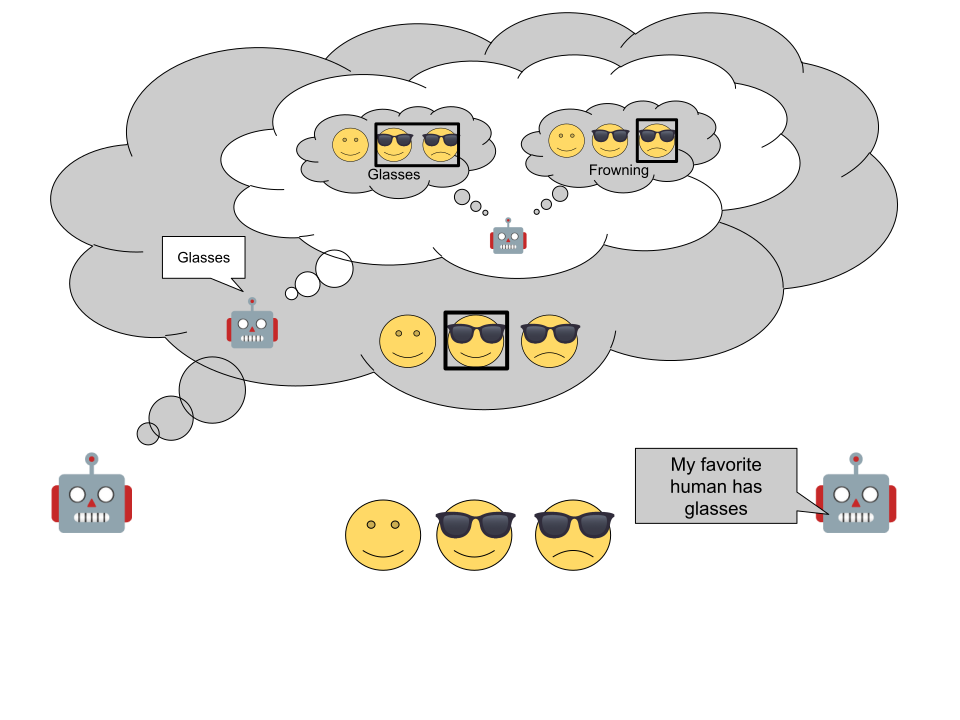
\includegraphics[width=0.9\textwidth, , trim=0 150 0 0, clip]{rsa_diagram.png}
    \caption{A diagram illustrating the recursive reasoning in the RSA framework. Adapted from \cite{Goodman2016} and \cite{Yuan_Monroe_Bai_Kushman}.}
    \label{fig:rsa_diagram}
\end{figure}

\subsection{Soft Actor-Critic (SAC)}
A central algorithm in modern, model-free reinforcement learning, particularly for continuous control tasks, is \textbf{Soft Actor-Critic (SAC)} \cite{Haarnoja2018}. SAC is an off-policy, actor-critic algorithm built upon the maximum entropy reinforcement learning framework. The core idea of this framework is to augment the standard objective of maximizing expected cumulative reward. The agent is additionally incentivized to maximize the entropy of its policy, effectively learning to succeed at the task while acting as randomly as possible. This entropy-maximization objective provides significant practical benefits, including improved exploration and enhanced robustness.

The algorithm's derivation is based on soft policy iteration, which alternates between evaluation and improvement steps. The soft policy evaluation step uses a modified Bellman backup operator to compute a "soft" Q-value, which incorporates both the external reward and the policy's entropy. The soft policy improvement step then updates a stochastic policy (the actor) to minimize its KL-divergence to the exponential of this new soft Q-function. The practical, deep reinforcement learning version of SAC uses neural networks to represent the actor and critic \cite{Haarnoja2018}. To further improve stability and mitigate the common problem of Q-value overestimation, SAC utilizes a "clipped double Q" technique, learning two independent Q-functions and using the minimum of their values in the update targets. This combination of off-policy data reuse, entropy maximization, and a stochastic actor results in an algorithm known for its high sample efficiency and stable convergence properties.

\section{Related Work}

\subsection{Collaborative Rational Speech Act (CRSA)}
Recent extensions to the RSA framework have sought to move beyond static, single-turn interactions to model more complex, dynamic settings. A notable example is the \textbf{Collaborative Rational Speech Act (CRSA)} framework \cite{Estienne2025}, an information-theoretic extension of RSA designed specifically for multi-turn, collaborative dialogs. This model addresses scenarios where agents must reason about shared goals and beliefs while holding different private information.

CRSA formalizes this by optimizing a multi-turn gain function, adapted from rate-distortion theory, that explicitly conditions on the dialog history ($w_t$). This allows the model to jointly track an agent's belief about both the shared task target and, crucially, their interlocutor's private knowledge. This work shares a core objective with methods like the Bayesian Action Decoder (BAD) \cite{BayesAD}, as both provide a formal mechanism for agents to update beliefs about a partner's hidden state within a cooperative, partially observable task. While CRSA \cite{Estienne2025} is demonstrated in the linguistic domain---modeling referential games and doctor-patient conversations ---its theoretical grounding for belief-tracking in goal-driven, sequential interactions provides a direct parallel to the problem of action legibility. It can be viewed as a formal, language-based counterpart to the framework proposed in this thesis, which applies pragmatic reasoning to physical actions in a MARL context.

\subsection{Intrinsic Motivation in MARL}
Our work is a form of intrinsic motivation, but it is critical to distinguish it from other methods, such as those based on social influence.

\subsubsection{Social Influence}
For example, \textbf{Social Influence} \cite{Jaques2019} provides an intrinsic reward for having a "causal influence over other agents' actions". This influence is assessed using counterfactual reasoning: at each timestep, an agent "simulates alternate actions that it could have taken, and computes their effect on the behavior of other agents" \cite{Jaques2019}. Actions that lead to bigger changes in others' behavior are rewarded, a mechanism shown to be "equivalent to rewarding agents for having high mutual information between their actions" \cite{Jaques2019}. While this method "leads to enhanced coordination and communication" and can be computed in a "decentralized way by enabling agents to learn a model of other agents" \cite{Jaques2019}, it explicitly incentivizes an agent to \textit{alter} the behavior of its peers.

\subsubsection{Theory of Mind as Intrinsic Motivation}
Another approach within intrinsic motivation is to use \textbf{Theory of Mind (ToM)} itself as the reward source. 
Rather than rewarding an agent for influencing another's external actions, this line of research rewards an agent for reasoning about the internal beliefs of other agents \cite{oguntola2023theory}. 
For instance, some work proposes that an agent's ability to accurately predict the beliefs of its partners can serve as a direct intrinsic reward signal \cite{oguntola2023theory}.

This method is built on the research question of whether ``modeling other agents' beliefs can serve as an intrinsic reward signal to improve performance'' \cite{oguntola2023theory}. 
The intrinsic reward is thus derived from second-order belief prediction \cite{oguntola2023theory}.

\subsubsection{Information as Regularizer}
Alternative approaches have utilized information-theoretic principles to explicitly manage an agent's disclosure of its internal state. Strouse et al. \cite{NEURIPS2018_1ef03ed0} introduce an information regularization framework where agents are trained to either reveal or conceal their intentions in an asymmetric information game. This is achieved by adding a regularizer to the policy gradient objective based on the mutual information between the agent's goal and its actions ($I(A;G|S)$) or states ($I(S;G)$) \cite{NEURIPS2018_1ef03ed0}. The cooperative aspect of their framework, which encourages maximizing this mutual information to share intentions, aligns closely with our own objective of enhancing legibility \cite{NEURIPS2018_1ef03ed0}. However, their work also formalizes the inverse problem: by inverting the sign of the regularizer, their agents learn competitive policies that actively *hide* intentions from an observer \cite{NEURIPS2018_1ef03ed0}. Their approach can thus be seen as formalizing both legibility and its adversarial counterpart, treating the two as opposite sides of a unified information-theoretic objective \cite{NEURIPS2018_1ef03ed0}.

\subsection{Bayesian Theory of Mind (ToM)}
Another related area is computational \textbf{Bayesian Theory of Mind (ToM)} \cite{Rabinowitz2018}, which involves explicitly modeling how an observer reasons about an agent's unobserved mental state, such as its desires, beliefs, and intentions. Modern implementations, such as the ToMnet proposed by \cite{Rabinowitz2018}, use meta-learning to build a strong prior model of other agents. This allows them to bootstrap from only a small number of behavioural observations to make richer predictions about an agent's characteristics and mental states. A key benchmark for such systems is passing classic ToM tasks, such as the 'Sally-Anne' test, which requires recognizing that others can hold false beliefs about the world \cite{Rabinowitz2018}.

\subsection{Bayesian Action Decoder (BAD)}
A notable framework that operationalizes this style of ToM reasoning is the \textbf{Bayesian Action Decoder (BAD)} \cite{BayesAD}. BAD is a multi-agent method designed for cooperative, partially observable settings where agents must ``discover effective strategies and conventions'' \cite{BayesAD}. The core mechanism involves agents
maintaining a ``public belief'' over the environment's hidden state, which is updated via approximate Bayesian inference. This update process, which ``is closely related to the theory of mind reasoning'' \cite{BayesAD}, allows agents to infer their partners' private information from their observed actions. A key aspect of this method is its use of ``counterfactual reasoning'' \cite{BayesAD}: the belief update considers not just the action an agent took, but also the alternative actions they \textit{could have} taken given different private information. This allows the team to ``discover effective communication protocols'' \cite{BayesAD}. This approach was subsequently refined by the \textbf{Simplified Action Decoder (SAD)} \cite{Hu_Foerster_2021}, which addresses a core conflict between standard RL exploration and communicative informativeness. SAD resolves this by leveraging the centralized training phase, allowing agents to observe both the \textit{exploratory} action and the \textit{greedy} action of their teammates, thereby providing a clearer signal about their underlying policy \cite{Hu_Foerster_2021}.

\subsection{Off-Belief Learning and Grounded Policies}
A significant challenge in cooperative MARL is the tendency for agents trained via self-play to develop arbitrary, yet efficient, conventions. These conventions are fragile and lead to poor performance when an agent is paired with a novel partner, such as a human or an independently trained agent, a problem formalized as Zero-Shot Coordination (ZSC). \textbf{Off-Belief Learning (OBL)} \cite{Hu_Lerer_Cui_Wu_Pineda_Brown_Foerster_2021} was introduced as a method to address this by explicitly controlling the cognitive reasoning depth of agents. The core mechanism of OBL trains a policy, $\pi_1$, under a "counterfactual" assumption: at each step, the agent assumes all \textit{past} actions were taken by a fixed, simple policy (e.g., uniform random $\pi_0$), but that all \textit{future} actions will be taken by its own optimal policy $\pi_1$. This procedure prevents the reliance on inferred conventions and forces the agent to learn an \textit{optimal grounded policy} that relies only on information explicitly revealed by the environment. Unlike related concepts such as Cognitive Hierarchies, OBL's assumption of optimal future play allows it to learn "grounded signaling"---taking costly actions to reveal information, knowing its partner will be rational enough to use it. This process can be iterated to create a hierarchy of policies with controlled cognitive depth, and its convergence to a unique policy makes it a suitable solution for ZSC \cite{Hu_Lerer_Cui_Wu_Pineda_Brown_Foerster_2021}.

\subsection{Inverse Reinforcement Learning (IRL)}
Conceptually, our work is related to \textbf{Inverse Reinforcement Learning (IRL)} \cite{ARORA2021103500} \cite{ziebart2008maximum}, which also seeks to infer latent causes (like a reward function) from observed behavior. IRL typically aims to recover a single, global, static reward function that explains an agent's entire policy, often for imitation or analysis.

\section{Critical Discussion: Limitations of Existing Work}
The current state of the art, while advancing coordination, leaves a critical gap that this thesis aims to fill. Standard MARL agents remain optimized only for task success, resulting in opaque policies that fail in settings requiring predictability. The existing methods that address this opacity, legibility, or coordination do so with different objectives and mechanisms than the framework proposed herein.

A significant body of work, including Bayesian Theory of Mind \cite{Rabinowitz2018} and the Bayesian Action Decoder \cite{BayesAD}, has focused on developing a sophisticated \textit{observer}. These methods provide formal mechanisms for an agent to interpret its partner's actions or infer their latent mental states. Our work addresses the complementary problem: how an \textit{actor} can prospectively shape its own behavior to make this Bayesian inference as clear and accurate as possible for its partner. Similarly, Inverse Reinforcement Learning \cite{ARORA2021103500} operates at the wrong level of abstraction; it aims to recover a global reward function from an entire policy, rather than providing an immediate, online signal to an agent to improve the communicative clarity of a single action.

Within the field of intrinsic motivation, common approaches are ill-suited for this specific cooperative goal. For example, rewards based on "social influence" \cite{Jaques2019} fundamentally miss the objective of legibility. They reward an agent for \textit{coercing} a partner into changing their policy. Our work addresses a different, more cooperative goal: rewarding an agent for the \textit{informative} act of clearly revealing its \textit{own} private state, regardless of how its partner subsequently uses that information. Other methods that use Theory of Mind as a reward \cite{oguntola2023theory} incentivize agents to make their beliefs \textit{predictable}. This is distinct from our goal of making an agent's actions pragmatically \textit{informative} about a specific, latent intention.

Perhaps the most direct conceptual competitors are methods that explicitly regularize a policy for information disclosure. Strouse et al. \cite{NEURIPS2018_1ef03ed0}, for instance, use a mutual information regularizer, $I(A;G|S)$, to encourage actions $A$ that reveal a goal $G$. The framework proposed in this thesis differs in its philosophical and computational foundation. A mutual information objective measures statistical correlation, whereas our RSA-based reward models a process of \textit{pragmatic inference}. It quantifies the clarity of an action by reasoning about the \textit{alternatives} the agent could have taken and the relative \textit{costs} of those actions, a richer model of communication than statistical dependence alone.

Finally, our work shares a high-level objective with methods like Off-Belief Learning (OBL) \cite{Hu_Lerer_Cui_Wu_Pineda_Brown_Foerster_2021}, which also seek to produce "grounded" policies suitable for Zero-Shot Coordination. However, the mechanisms are distinct. OBL achieves grounding by controlling the cognitive reasoning depth of agents during training, forcing them to learn policies that are optimal when playing with a simpler, baseline partner. Our framework, in contrast, proposes to achieve this grounding by providing an explicit, intrinsic reward ($\Rcomm$) that is itself derived from a formal model of pragmatic interpretation. This thesis posits that providing a direct incentive for legibility is a more direct and flexible method for generating such grounded, cooperative policies. Our framework thus provides a formal mechanism to bridge instrumental planning with communicative intent, a concept not adequately addressed by prior work.


%---------------------------------------------------------------------
%   5. COMPANY/LAB PRESENTATION (2 pages)
%---------------------------------------------------------------------
\chapter{Professional Context}

This thesis was conducted within the dynamic artificial intelligence ecosystem of Montreal, Quebec, and was supported by a combination of French and Canadian institutions.

\section{Presentation of the Host Laboratories}

Formally, I was employed as a researcher by the CNRS (Centre National de la Recherche Scientifique), France's national public research organization. My host laboratory was the International Laboratory on Learning Systems (ILLS) \cite{CNRS_Ottawa_2025}. ILLS is an International Research Laboratory (IRL) and consortium designed to foster collaboration between French institutions (including CNRS and CentraleSupélec) and Canadian partners (including McGill University and Mila).

\section{Team, Projects, and Assigned Mission}

The research structure at ILLS is characterized by thematically related, yet highly independent, research programs. Reflecting this, my work was not part of a single, large, project-oriented team. Rather, the environment consisted of affiliated researchers pursuing independent, though often complementary, lines of inquiry.

Correspondingly, this thesis did not originate from a pre-defined, top-down project or a formally "assigned mission." The work was, by design, exploratory and open-ended. The project's inception point was a formal observation: the striking mathematical similarity between the optimal policy formulations in Maximum Entropy Reinforcement Learning (Max-Ent RL) and the "speaker" models used in computational pragmatics.

The mission, therefore, was to investigate this formal bridge—to determine if it was a mere coincidence or if it could be operationalized as a new, principled framework for multi-agent coordination. This made the research fundamentally curiosity-driven, focused on theoretical connections and their potential applications.

\section{Position of the Thesis within this Context}

My other intellectual and scientific home for this work was Mila -- Quebec AI Institute \cite{Mila}. Through my supervisor, Pablo Piantanida, I was a formally affiliated researcher at Mila and visited the institute's offices weekly.

This affiliation provided the ideal environment for such an exploratory topic. Given Mila's scale and breadth, the institute hosts a high concentration of researchers working on all the component parts of this thesis, including multi-agent systems, intrinsic motivation, and probabilistic models of language. While my specific theoretical bridge was novel, I was ableto draw upon this vast pool of resident expertise.

This affiliation was not a simple formality; it was the most significant scientific influence on this thesis. It granted me full immersion into a dense and active research community. I was a regular participant in the RL reading groups, informally known as the "RL Couch," where discussions on recent papers helped refine the methodological foundations of my work.

Beyond my specific sub-field, the breadth of seminars was critical for providing new perspectives. For instance, I attended highly technical talks, such as one on the "Tiny Recursive Model," \cite{jolicoeur2025less} as well as foundational discussions, like a talk by Professor Yoshua Bengio on the long-term societal risks of AI. This context allowed the thesis to be positioned at an intersection: grounded in the fundamental research focus of CNRS/ILLS, but developed, challenged, and refined through the dynamic, large-scale, and feedback-rich ecosystem of Mila.


%---------------------------------------------------------------------
%   6. PROBLEM DESCRIPTION (4 pages)
%---------------------------------------------------------------------
\chapter{Problem Description}

\section{Precise Formulation of the Problem}
From a formal perspective, a standard Reinforcement Learning (RL) agent is modeled as an optimizer within a Markov Decision Process (MDP). Its objective $J(\pi)$ is to find a policy $\pi(a_t | s_t)$ that maximizes the expected, discounted sum of future external rewards:
$$ J(\pi) = \mathbb{E}_{\tau \sim \pi} \left[ \sum_{t=0}^T \gamma^t \Rext(s_t, a_t) \right] $$
where $\tau$ is a trajectory $(s_0, a_0, s_1, a_1, \dots)$ generated by the policy.

The core of our research problem lies in the fact that this objective is fundamentally \textit{agnostic} to the interpretability of the resulting behavior. An agent optimizing only for $\Rext$ has no incentive to select an action that is "legible" or "unambiguous" to a cooperative partner, as discussed in the 'Simple Spread' example. This ambiguity can be formalized. Let an agent possess a private state $m_t \subset s_t$, such as its intended target landmark. An observer---a teammate---attempts to infer this private state by observing the agent's action $a_t$, forming a posterior belief $P(m | a_t)$. The action $a_t$ is ambiguous if this posterior distribution is diffuse (i.e., has high entropy), and it is legible if the distribution is sharp, assigning high probability to the true state $m_t$.

The standard objective $J(\pi)$ provides no mechanism to encourage the latter. To address this, we propose that a cooperative agent must optimize a composite objective. We introduce a novel, intrinsic \textbf{communicative reward}, $\Rcomm$, which mathematically quantifies the legibility of an action. This reward is defined as the information an action $a_t$ provides about the agent's true private state $m_t$, as interpreted by a rational listener.

Our central proposition is to reformulate the agent's optimization problem. The agent should learn a policy $\pi$ that maximizes a total, composite reward function, $R_{total}$, at every timestep:
$$ R_{total}(s_{t},a_{t}) = \Rext(s_{t},a_{t}) + \lambda \Rcomm(a_t; m_t) $$
Here, $\Rext$ remains the external task reward, $\Rcomm(a_t; m_t)$ is the intrinsic communicative reward for taking action $a_t$ given the private state $m_t$, and $\lambda$ is a hyperparameter that balances the trade-off between task optimality and communicative clarity.

This formulation focuses the entire research challenge onto a single, precise question: How can $\Rcomm$ be defined and computed in a principled, theoretically-grounded, and efficient manner? This thesis posits that the answer lies in bridging the mathematics of computational pragmatics with the framework of modern reinforcement learning.

\section{Working Hypotheses}
Our work is guided by the following hypotheses:
\begin{enumerate}
    \item \textbf{Formal Equivalence:} A formal equivalence exists between the optimal policy solution in single-step Max-Ent RL and the "speaker" model in the RSA framework.
    \item \textbf{Principled Reward:} This equivalence allows us to "import" the "listener value" ($\VL$) from RSA to serve as a principled intrinsic reward ($\Rcomm$) for legibility.
    \item \textbf{Improved Legibility:} Training an agent to maximize $\Rtotal$ will produce policies that are measurably more legible (i.e., an observer can more accurately infer $m_t$ from $a_t$).
    \item \textbf{Improved Performance:} This increased legibility will lead to more effective team coordination and higher task performance.
\end{enumerate}

\section{Data Used: Environments and Scenarios}
Our primary experimental testbed is a modified version of the \texttt{Simple Spread} scenario, drawn from the Multi-Agent Particle Environments (MPE) suite \cite{lowe2017multi}, \cite{mordatch2017emergence}. We specifically utilize the \texttt{VectorizedMultiAgentSimulator} (VMAS) implementation of this environment \cite{bettini2022vmas}. This choice was a methodological one, driven primarily by performance considerations. The VMAS framework is designed for high-throughput, GPU-based parallelization, which is essential for our training methodology as it allows for a large number of environments to be simulated concurrently.

\subsection{Modified Simple Spread}
The \texttt{Simple Spread} scenario, in its standard form, is a foundational multi-agent coordination benchmark. It consists of $N$ agents and $N$ landmarks in a two-dimensional world. The agents' collective objective is to ``cover'' all landmarks simultaneously. The team reward is based on the proximity of agents to the landmarks, calculated as the sum of distances from each landmark to its nearest agent. A penalty is also applied for collisions between agents to encourage spatial separation.

We introduce a significant modification to this standard scenario to create a testbed for cooperative partial observability and intent. In our version, both agents and landmarks are assigned ``categories'' or ``types''. Each agent $i$ possesses a private ``meaning'' or ``preference'' $m_i$ (e.g., preference for 'blue'). The set of landmarks $L$ is populated with $N$ landmarks, each with a corresponding 'category' (represented by colors).

The rules of this modified environment are as follows: The team receives a positive preference bonus for each landmark that is covered by an agent whose private preference $m_i$ matches the landmark's property. This bonus is offset by a distance penalty, equal to the sum of distances from each landmark to its single closest agent, which incentivizes the team to cover \textit{all} landmarks. A collision penalty is also applied to discourage uncoordinated movement. This structure creates a complex coordination challenge: an agent's private preference $m_i$ is its hidden state, and it must act not only to cover its preferred landmark but also to legibly signal its intent so that teammates can confidently pursue \textit{other} landmarks, thereby minimizing the team's total distance penalty.

\begin{figure}[h!]
    \centering
    
    % --- We use minipages to place images and their labels side-by-side ---
    
    \begin{minipage}{0.32\textwidth}
        \centering
        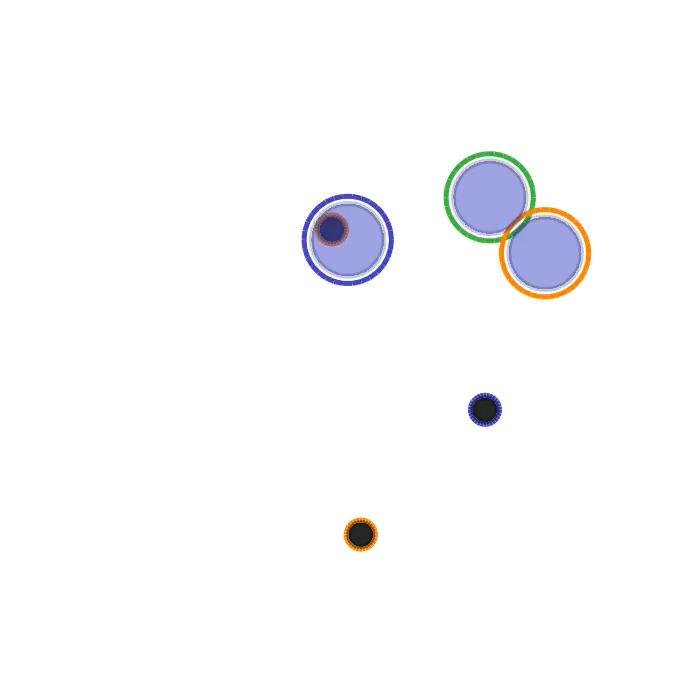
\includegraphics[width=\linewidth, keepaspectratio]{snapshot.jpg}
        \centerline{Episode Start}
    \end{minipage}
    \hfill % Adds horizontal space
    \begin{minipage}{0.32\textwidth}
        \centering
        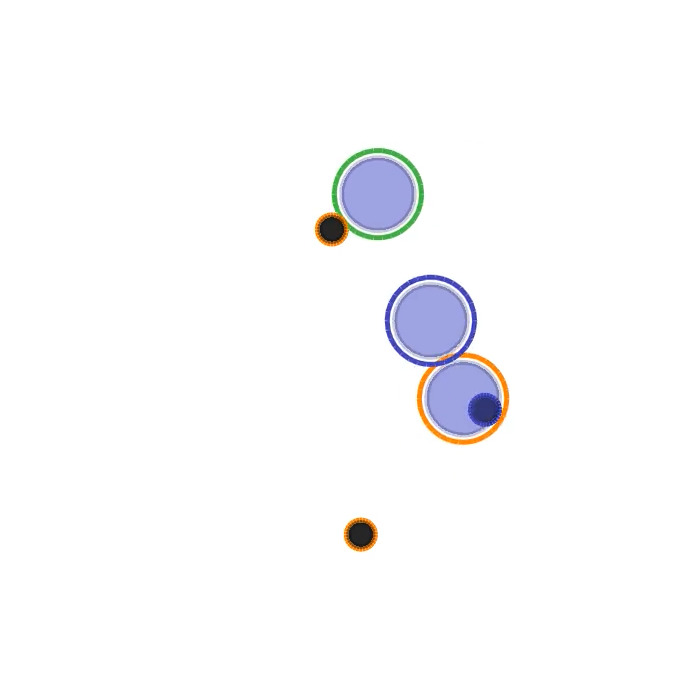
\includegraphics[width=\linewidth, keepaspectratio]{snapshot2.jpg}
        \centerline{Episode Middle}
    \end{minipage}
    \hfill % Adds horizontal space
    \begin{minipage}{0.32\textwidth}
        \centering
        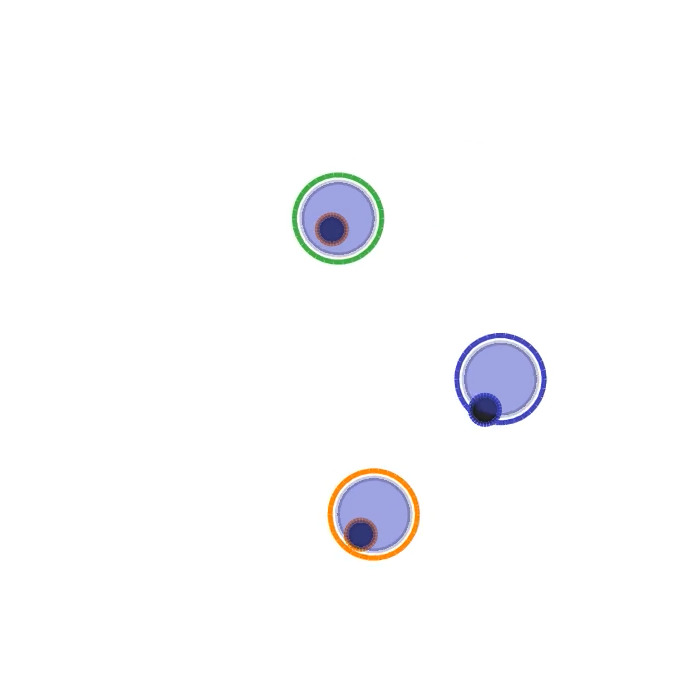
\includegraphics[width=\linewidth, keepaspectratio]{snapshot3.jpg}
        \centerline{Episode End}
    \end{minipage}
    
    \vspace{5pt} % Adds a small vertical space before the main caption

    % --- Caption with integrated TiKZ Legend ---
    % \protect is needed before \tikz inside a caption to prevent errors
    \caption{
        A single episode in the 'Simple Spread' environment.
    }
    \label{fig:simple_spread_episode}
\end{figure}

\subsection{Action and Observation Spaces}
The environment is defined by continuous action and observation spaces. The action space $\mathcal{A}$ for each agent $i$ is continuous and defined as a 2-dimensional vector $a_i \in [-1, 1]^2$. This vector represents the physical force applied by the agent in the $x$ and $y$ dimensions at each discrete timestep. There is no explicit communication channel; all signaling must be accomplished emergently through these physical actions.

The base observation space $\mathcal{O}$ is also a continuous vector, providing each agent with its own state and information about the environment. This vector includes the agent's absolute position, its velocity, its private intention $m_i$ (encoded as a one-hot vector), the relative positions to all landmarks, the one-hot encoded properties of all landmarks, and the relative positions to all other agents. The composition of this observation is further defined by the specific experimental condition.

To evaluate the impact of legibility under different informational settings, we test two primary experimental conditions. The first is the \textbf{Belief-Augmented Observation} condition, where each agent's observation includes not only its own private intention ($m_i$) but also its current beliefs about the intentions of all its teammates. This primarily serves as a "best-case" baseline in which agents can easily assign themselves an optimal target. The second, more challenging condition is the \textbf{Local-Intention Observation}. In this setting, an agent sees only its own intention ($m_i$) and must infer the intentions of its partners purely from their observed actions. This latter condition provides a stricter test of our framework, as effective coordination is critically dependent on the emergence of legible, communicative actions.

\subsection{Alternative Environments Considered}
In the course of our research, we also experimented with more complex, mixed-motive MPE environments, such as \texttt{Simple Tag}. In this scenario, a team of ``protagonist'' agents must learn to coordinate their pursuit to capture one or more ``adversary'' agents, who are also learning an evasion policy. While this environment introduces a rich adversarial dynamic, we ultimately focused our analysis on the cooperative \texttt{Simple Spread} task. This decision was made to reduce extraneous variability in the training signal. Training a \texttt{Simple Tag} model would require concurrently training two distinct sets of policies, introducing a significant computational overhead and making it more difficult to isolate the specific impact of our proposed pragmatic reward on \textit{cooperative} legibility.

Furthermore, our selection of the MPE suite was deliberate, foregoing other common MARL benchmarks such as the cooperative card game Hanabi. While Hanabi serves as a canonical testbed for emergent communication and coordination under partial observability, its discrete, high-dimensional state space and significant strategic complexity were deemed outside the immediate scope of this investigation. A primary objective of this work was to provide clear, visually intuitive, and human-readable examples of how pragmatic reasoning can function as an intrinsic motivation within an RL framework. The continuous, 2D-particle environments are ideally suited for this purpose, as they permit direct qualitative analysis of emergent physical trajectories and spatial strategies, which clearly illustrate the behavioral impact of the pragmatic reward.


%---------------------------------------------------------------------
%   7. METHODOLOGY (8 pages)
%---------------------------------------------------------------------
\chapter{Methodology}

\section{The Proposed Framework: A Hybrid Architecture}
Our model employs a hybrid architecture that formalizes and separates the concerns of long-term strategic planning from immediate-turn pragmatic reasoning. The core of the framework is a primary Reinforcement Learning (RL) agent responsible for sequential planning. We implement this agent using Multi-Agent Soft Actor-Critic (MASAC), an algorithm well-suited for cooperative tasks requiring coordination. This agent learns its policy $\pi(a_t | s_t)$ by maximizing a total reward signal, which is a combination of standard external task rewards ($\Rext$) and a novel intrinsic reward, $\Rcomm$.

This intrinsic reward, $\Rcomm$, is computed by a separate \textbf{Pragmatic Reward Module (PRM)}. This module is designed to quantify the immediate communicative value, or "clarity," of an agent's action $a_t$ given its private state $s_t$. Crucially, the PRM is a component queried only \textit{during training} to compute $\Rcomm$ for a given transition $(s_t, a_t)$. This allows the agent to learn a policy that is both task-optimal and pragmatically effective, without adding any computational latency during decentralized execution.

\begin{figure}[h!]
    \centering
    
    % --- Define styles (same as before) ---
    \tikzset{
        block/.style={      % Style for Agent/Env blocks
            rectangle, 
            draw, 
            thick, 
            fill=gray!10, 
            rounded corners, 
            minimum height=2cm, 
            minimum width=3.5cm,
            text width=3.5cm,
            align=center,
            font=\large
        },
        prm_block/.style={  % Style for our PRM block
            block,
            fill=blue!10, % Differentiate it
            text width=5cm,
            minimum width=5cm
        },
        arrow/.style={      % Style for standard exec arrows
            draw, 
            thick, 
            -Stealth[]
        },
        prm_arrow/.style={  % Style for training-only arrows
            arrow,
            dashed
        }
    }
    
    \begin{tikzpicture}[
        auto,
        >=Stealth,
    ]
        % --- Nodes in a triangular layout ---
        \node[block] (agent) {\textbf{Agent}};
        
        \node[block, below left=of agent, node distance=10cm and 3cm] (env) {
            \textbf{Environment}
        };
        
        \node[prm_block, below right=of agent, node distance=10cm and 3cm] (prm) {
            \textbf{Pragmatic Reward Module (PRM)}
        };
        
        % --- Edges (Arrows) ---
        
        % 1. Agent <-> Environment Loop (Solid)
        \path [arrow] (agent.west) edge[bend right=25] 
            node[midway, above left, font=\large, xshift=-5mm] {Action $A_t$} (env.north);
        
        \path [arrow] (env.east) edge[bend right=25] 
            node[midway, below right, font=\large, xshift=-2mm, yshift=-2mm] {
                State $S_{t+1}$, 
                \textbf{$\Rext$}
            } (agent.south west);
            
        % 2. Agent <-> PRM Loop (Dashed)
        \path [prm_arrow] (agent.east) edge[bend left=25]
            node[midway, above right, font=\large, xshift=5mm] {
                Action $A_t$, 
                $m_t$
            } (prm.north);
            
        \path [prm_arrow] (prm.west) edge[bend left=25]
            node[midway, below left, font=\large, xshift=0mm, yshift=7mm] {
                \textbf{$\Rcomm$}
            } (agent.south east);

        \path [prm_arrow] (env.south) edge[bend right=25]
            node[midway, below left, font=\large, xshift=0mm, yshift=0mm] {
                State $S_{t}$
            } (prm.south);
            
    \end{tikzpicture}
    
    \caption{
        The augmented training loop with the Pragmatic Reward Module (PRM) in a triangular configuration. 
        The solid arrows represent the standard execution loop: the agent takes $A_t$, and the environment returns $S_{t+1}$ and the task-specific \textit{external reward} $\Rext$.
        The dashed arrows represent the \textit{centralized training} process: the PRM observes the agent's action and private state $m_t$ to compute the \textit{communicative reward} $\Rcomm$. While it needs the state $S_{t}$ to calculate these rewards, it does not "step" the environment.
        The agent's policy is then updated using the total reward $\Rtotal = \Rext + \lambda \Rcomm$.
    }
    \label{fig:prm_loop_triangle}
\end{figure}

\section{The Theoretical Bridge: Unifying Max-Ent RL and RSA}
The foundation of our hybrid framework is the formal equivalence between the classic, static Rational Speech Act (RSA) framework and a single-step Maximum Entropy Reinforcement Learning (Max-Ent RL) problem. We establish a direct mapping between the components of both models. The RL State ($s$), or more specifically the agent's private information, corresponds to the RSA Meaning ($m$) to be communicated. The RL Action ($a$) maps to the RSA Utterance ($u$), and the RL Policy ($\pi(a|s)$) maps to the RSA Speaker model ($S(u|m)$).

Most importantly, this equivalence allows us to formally define our intrinsic reward. The RL Reward ($R(s,a)$) is shown to be a direct analogue of the RSA \textbf{Listener Value ($V_L(u,m)$)}, which quantifies the utility of an action (utterance) for conveying a specific state (meaning). The optimal Max-Ent RL policy is a softmax distribution over rewards, $\pi^{*}(a|s)\propto \exp(R(s,a)/\alpha_{RL})$, just as the RSA speaker model is a softmax over the listener value, $S(u|m)\propto \exp(\alpha_{RSA}\cdot V_{L}(u,m))$. The two formulations are equivalent under the re-indexing $\alpha_{RSA}=1/\alpha_{RL}$, allowing us to define our communicative reward as $\Rcomm \triangleq \VL$.

\section{Calculating the Pragmatic Reward}
Based on this theoretical bridge, we define the intrinsic pragmatic reward $\Rcomm$ that the PRM provides to the RL agent. This reward is precisely the listener value derived from the RSA component. For a given state-action pair $(s_t, a_t)$, where the agent's private state (or meaning) is $m_{S_t}$, the reward is:
$$ \Rcomm(s_{t},a_{t}) \triangleq \VL(a_{t},m_{S_{t}}) = \log L_{t}^{*}(m_{S_{t}}|a_{t}) - C(a_{t}) $$
This formulation is identical to the 'immediate reward' term used in the dynamic RSA-Bellman equation. The term $L_{t}^{*}(m_{S_{t}}|a_{t})$ represents the "clarity" of the action: the probability a rational listener would assign to the agent's true state $m_{S_t}$ after observing action $a_t$. $C(a_t)$ is an optional cost associated with the action.

\subsection{The Literal Listener ($L_0$) Model}
To compute this reward, the PRM must instantiate a listener model. This process begins by defining a "literal listener," $L_t^0$, which serves as the 0-level starting point for pragmatic reasoning. The implementation of this $L_0$ model is flexible; it can be a simple, computationally cheap heuristic (e.g., a shortest-path preference), the agent's own policy $\pi$ (to measure legibility relative to its own habits), or a separately trained Theory of Mind (ToM) network.

The choice of this $L_0$ model is perhaps the most crucial free parameter in the framework, as it fundamentally defines the \textit{assumed common ground} for communication. It is the baseline against which the "informativeness" or "clarity" of an action $a_t$ is measured. This $L_0$ is the direct analogue to the "literal listener" in the Rational Speech Act (RSA) framework, which serves as the 0-level starting point for recursive pragmatic reasoning. In computational linguistics, the $L_0$ interprets utterances literally. In our framework, the $L_0$ interprets \textit{behavior} "literally"---for example, by assuming the agent is a simple, non-communicative optimizer.

The complexity of the $L_0$ model has a direct impact on the nature of the legibility it encourages. A simple heuristic like a shortest-path preference is computationally cheap, but it creates a static baseline; legibility is achieved by any "costly" deviation from this simple path. Using the agent's own policy $\pi$ as the $L_0$ is more complex, creating a dynamic baseline where legibility means acting in a way that is "unusually clarifying" relative to one's own established habits. The ToM network is the most sophisticated, modeling the beliefs of a specific partner, but also the most computationally costly.

In our framework, we operationalize this "shortest-path preference" as a specific, computationally-efficient heuristic. This $L_0$ model serves as a "naive listener" that interprets actions based on their geometric similarity to ideal paths. For any given agent $i$ taking action $a_i$, the listener's belief $L_0(m|a_i)$ over the set of all possible meanings $\mathcal{M}$ (i.e., target categories) is computed. First, for each possible meaning $m \in \mathcal{M}$, the model identifies the \textit{closest} landmark $l_m$ of that category and computes the ideal direction vector $v_m$ from the agent's position $\text{pos}_i$ to the landmark's position $\text{pos}_{l_m}$.

A simple $L_0$ might define a score as $S(a_i, m) = \cos(a_i, v_m)$. However, to better capture the notion of unambiguity, our $L_0$ model computes an \textbf{exclusivity score}. This score explicitly penalizes similarity to competing meanings:
$$ S_{\text{excl}}(a_i, m) = \alpha_{\text{temp}} \left( \cos(a_i, v_m) - \max_{m' \neq m} \cos(a_i, v_{m'}) \right) $$
where $\alpha_{\text{temp}}$ is the listener's temperature hyperparameter (\texttt{pragmatic\_temp}). This score is high only if the action $a_i$ is significantly more aligned with the ideal path $v_m$ than with the ideal path $v_{m'}$ for \textit{any other} "confusable" meaning. The final $L_0$ belief is the softmax over these exclusivity scores:
$$ L_0(m | a_i) = \frac{\exp(S_{\text{excl}}(a_i, m))}{\sum_{m'' \in \mathcal{M}} \exp(S_{\text{excl}}(a_i, m''))} $$
The importance of this specific formulation is profound. A poorly defined $L_0$, such as a uniform distribution, would fail to provide a useful signal. If an agent takes a "corralling" path to be clear, this action is just as (un)surprising to a uniform $L_0$ as the ambiguous shortest path. The informative deviation is not recognized, and $\Rcomm$ remains near zero. In contrast, our "exclusivity" $L_0$ \textit{expects} actions to be somewhat aligned with their goals. When an agent takes an ambiguous shortest path (similar to both $v_m$ and $v_{m'}$), the $\max$ term is large, $S_{\text{excl}}$ is low, and the resulting $L_0$ distribution is flat, leading to a low pragmatic reward. To achieve a high reward, the agent must choose an $a_i$ that maximizes $\cos(a_i, v_m)$ while simultaneously \textit{minimizing} $\cos(a_i, v_{m'})$ for all $m' \neq m$, thereby reinforcing clear, legible strategies.

\section{Pragmatic Reward Algorithm}
The complete flow of the Pragmatic Reward Module (PRM) at each training step $t$ is formalized in Algorithm 1. The module takes the current state and the agent's true action $a_{\text{true}}$ and true meaning $m_{\text{true}}$ as input. It first computes the $L_0$ model by comparing $a_{\text{true}}$ and $K$ other sampled "alternative" actions against the ideal direction vectors for all possible meanings. It then performs recursive RSA reasoning for $N_r$ iterations to compute a pragmatic listener belief $L_k$. The final reward, $\Rcomm$, is the log-probability this listener assigns to the agent's true meaning $m_{\text{true}}$ given its true action $a_{\text{true}}$.

\hspace{}

\begin{algorithm}[H]
\SetAlgoLined
\caption{Pragmatic Reward Module (PRM) Flow}
\label{alg:prm}
\SetKwInOut{Input}{Input}
\SetKwInOut{Output}{Output}

\Input{
    Agent $i$ with position $\text{pos}_i$;
    State $s_t$ (containing all landmark positions $P_L$ and types $T_L$);
    True action $a_{\text{true}}$ taken by agent $i$;
    True meaning $m_{\text{true}}$ of agent $i$;
    Set of all possible meanings $\mathcal{M}$;
    $K$: number of action samples (\texttt{pragmatic\_n\_samples});
    $N_r$: number of RSA iterations (\texttt{pragmatic\_n\_iterations});
    $\alpha_{\text{temp}}$: listener temperature (\texttt{pragmatic\_temp});
}
\Output{Pragmatic reward $\Rcomm$ for agent $i$}

\tcp{Step 1: Sample alternative actions}
$A_{\text{alt}} \leftarrow \text{SampleActions}(K, \text{action\_space})$\;
$A_{\text{all}} \leftarrow \{a_{\text{true}}\} \cup A_{\text{alt}}$ \tcp{Set of $K+1$ actions}

\tcp{Step 2: Compute ideal direction for each meaning}
\For{each meaning $m \in \mathcal{M}$}{
    $l_m \leftarrow \text{FindClosestLandmark}(m, \text{pos}_i, P_L, T_L)$\;
    $v_m \leftarrow \text{Direction}(\text{pos}_i, l_m.\text{pos})$\;
}

\tcp{Step 3: Calculate Literal Listener $L_0$ scores for all actions}
\For{each action $a \in A_{\text{all}}$}{
    \For{each meaning $m \in \mathcal{M}$}{
        $S(a, m) \leftarrow \alpha_{\text{temp}} \cdot \cos(a, v_m)$\;
    }
    \For{each meaning $m \in \mathcal{M}$}{
        $S_{\text{max\_other}} \leftarrow \max_{m' \in \mathcal{M}, m' \neq m} S(a, m')$\;
        $S_{\text{excl}}(a, m) \leftarrow S(a, m) - S_{\text{max\_other}}$\;
    }
    $L_0( \cdot | a) \leftarrow \text{Softmax}(S_{\text{excl}}(a, \cdot))$ \tcp{Belief dist. for action $a$}
}

\tcp{Step 4: Perform $N_r$ recursive RSA iterations}
$L_k \leftarrow L_0$\;
\For{$j \leftarrow 1$ \KwTo $N_r$}{
    $S_k(a | m) \leftarrow L_{k-1}(m | a) / \sum_{a' \in A_{\text{all}}} L_{k-1}(m | a')$ \tcp{Speaker $S_j$}
    $L_k(m | a) \leftarrow S_k(a | m) / \sum_{m' \in \mathcal{M}} S_k(a | m')$ \tcp{Listener $L_j$ (uniform $P(m)$)}
    $L_{k-1} \leftarrow L_k$\;
}

\tcp{Step 5: Calculate final pragmatic reward}
$L_{\text{final}} \leftarrow L_k( \cdot | a_{\text{true}})$ \tcp{Posterior belief for the *true* action}
$p_{\text{true}} \leftarrow L_{\text{final}}(m_{\text{true}})$ \tcp{Probability of the *true* meaning}
$\Rcomm \leftarrow \log(p_{\text{true}})$\;

\Return $\Rcomm$\;
\end{algorithm}

\section{Training Strategy: CTDE}
Our approach uses the Centralized Training with Decentralized Execution (CTDE) paradigm. During the centralized training phase, the Pragmatic Reward Module (PRM) is given "perfect access" to all agents' true private states ($m_t$). This allows it to compute a "gold-standard" $\Rcomm$ signal, which is used to update the agents' value functions. For decentralized execution, the trained agent executes its policy $\pi(a_t | s_t)$ using only its local observations, without needing access to the PRM or other agents' private states.

\section{The Strategic Bellman Equation}
By embedding this single-step reward mechanism into a full sequential decision-making process, we arrive at a strategic Bellman equation that guides the RL agent's learning. The agent's goal is to learn an action-value function, $Q_t(s_t, a_t)$, which represents the total expected future discounted value (reward + entropy) of taking action $a_t$ in state $s_t$. This Q-function is trained using the RSA-Specific Bellman Equation:

\begin{align*}
Q_{t}(s_{t},a_{t}) &= \Rtotal(s_{t},a_{t}) + \gamma\mathbb{E}_{s_{t+1}}\left[V_{t+1}(s_{t+1})\right] \\
&= (\Rext(s_{t},a_{t}) + \Rcomm(s_{t},a_{t})) + \gamma\mathbb{E}_{s_{t+1}}\left[\alpha \log\sum_{a_{t+1}}\exp\left(\frac{1}{\alpha}Q_{t+1}(s_{t+1},a_{t+1})\right)\right] \label{eq:bellman}
\end{align*}


Here, the immediate reward $\Rtotal$ is the sum of the external task reward $\Rext$ and our pragmatic reward $\Rcomm$, which is defined as $(log~L_{t}^{*}(m_{S_{t}}|a_{t})-C(a_{t}))$. The second term is the discounted, expected future value, where the optimal state-value function $V_{t+1}(s_{t+1})$ is the "soft-maximum" (or log-sum-exp) of the Q-values for the next state, $s_{t+1}$. This is the standard state-value definition in Max-Ent RL (see Appendix \ref{sec:v_derivation} for the full derivation).

This equation explicitly models the trade-off between immediate gains (both from the task and from clarity) and the long-term strategic value of future states. For instance, an agent might learn to take an action with a low immediate reward (e.g., a "corralling" motion) if it leads to a future state $s_{t+1}$ with a much higher expected value $V_{t+1}$.

Importantly, if we set the discount factor $\gamma=0$, the agent becomes "myopic," optimizing only for the immediate reward of the current turn. In this special case, the strategic Bellman equation collapses, and the Q-value $Q_t$ becomes identical to the immediate reward $R_t$. The agent's objective then becomes equivalent to maximizing the static, single-turn RSA gain function. This validates our framework as a true generalization of the classic RSA model (see Appendix \ref{sec:crsa_derivation} for a detailed derivation).

\section{Evaluation Metrics}
To comprehensively evaluate the performance and emergent behaviors of our framework, we employ a multi-faceted suite of metrics. These metrics are designed to answer three primary questions: (1) Does the team achieve the task objective effectively? (2) Does the team communicate clearly? and (3) What cooperative strategies emerge as a result of the pragmatic reward?

\subsection{Task Performance}
The primary measure of success is the mean Episodic Team Reward, which quantifies the team's ability to solve the cooperative task. This external reward, $\Rext$, is a composite signal computed at each timestep $t$:
$$ \Rext(t) = R_{pref}(t) - R_{dist}(t) - R_{coll}(t) $$
where:
\begin{itemize}
	\item $R_{pref}(t)$ is a positive reward granted for each landmark that is "covered" (i.e., is closest to) by an agent whose private preference (meaning $m_i$) matches the landmark's category. This encourages correct agent-landmark assignments.
	\item $R_{dist}(t)$ is a penalty equal to the sum of the Euclidean distances from each landmark to its single closest agent. This incentivizes the team to collectively minimize the distance to all landmarks, promoting full coverage.
	\item $R_{coll}(t)$ is a penalty applied when agents collide with one another, discouraging uncoordinated or crowded movements.
\end{itemize}
A higher cumulative $\Rext$ over an episode indicates superior task-level coordination and objective completion.

\subsection{Communicative and Cognitive Metrics}
We introduce several metrics to measure the quality, clarity, and coherence of the emergent communication.

\subsubsection{Communicative Clarity}
As pre-figured in the methodology, our primary measure of legibility is Communicative Clarity. This is the negative of the intrinsic reward $\Rcomm$ itself, averaged over the team. It is precisely the average cross-entropy between an agent's true, one-hot intention vector $m_i$ and the pragmatic listener's posterior belief distribution $L^*(m|a_i)$:
$$ \mathcal{L}_{\text{clarity}} = \frac{1}{N} \sum_{i=1}^N H(m_i, L^*(\cdot|a_i)) = - \frac{1}{N} \sum_{i=1}^N \log L^*(m_{\text{true}}^{(i)} | a_i) $$
This metric directly quantifies the success of the pragmatic reward signal. A lower value signifies that an agent's actions $a_i$ make its true intention $m_{\text{true}}^{(i)}$ highly probable to the rational listener, indicating high legibility.

\subsubsection{Literal Intent Accuracy}
We also measure "Literal Intent Accuracy". This metric assesses a more basic, non-pragmatic form of clarity by evaluating the $L_0$ model's "most likely" guess of the agent's intent. Let $L_0(m|a_i)$ be the literal listener's belief (a softmax over cosine similarities between the action $a_i$ and the direction to the nearest landmark of each meaning $m$). The predicted meaning is $\hat{m}_i = \arg\max_m L_0(m|a_i)$. The accuracy is:
$$ \text{Acc} = \frac{1}{|\mathcal{V}|} \sum_{i \in \mathcal{V}} \mathbb{I}(\hat{m}_i = m_{\text{true}}^{(i)}) $$
where $\mathbb{I}$ is the indicator function and $\mathcal{V}$ is the set of "valid" agents (those for whom a target landmark of their preferred category exists in the environment). This metric detects whether agents are, at a minimum, moving more towards their correct target category than any other.

\subsubsection{Team Belief Divergence}
To measure the coherence of the team's signaling, we calculate the Team Belief Divergence. This is the average Jensen-Shannon Divergence (JSD) between the literal belief distributions $L_0$ induced by the actions of all pairs of agents:
$$ \text{JSD}_{\text{team}} = \frac{1}{\binom{N}{2}} \sum_{i<j} \text{JSD}\left(L_0(\cdot|a_i) \parallel L_0(\cdot|a_j)\right) $$
where $L_0(\cdot|a_i)$ is the belief distribution $L_0(m|a_i)$ over all possible meanings $m$. A low JSD indicates a high level of "shared understanding" or "interpretive alignment" across the team, suggesting all agents are acting in ways that are literally interpreted similarly.

\subsection{Behavioral and Strategic Metrics}
Finally, we use a set of diagnostic metrics to understand the \textit{how}---the specific multi-agent strategies that emerge.

\subsubsection{Goal-Directedness}
We measure ''Goal-Directedness'' as the average cosine similarity between an agent's action $a_i$ and the vector $v_{\text{goal}}^{(i)}$ pointing to its true closest target landmark:
$$ \text{GD} = \frac{1}{|\mathcal{V}|} \sum_{i \in \mathcal{V}} \max\left(0, \cos(a_i, v_{\text{goal}}^{(i)})\right) $$
This metric quantifies how efficiently agents move towards their "literal" goal (clamped at 0 to ignore movement away from the goal). A low value, especially when paired with high task performance, can indicate a strategically legible policy (e.g., an agent taking a "detour" or "corralling" motion) that deviates from the most efficient path to be clearer.

\subsubsection{Team Specialization}
To quantify the emergence of a division of labor, we measure ''Team Specialization''. Let $T_i = \arg\min_{l \in \mathcal{L}_{m_i}} \text{dist}(\text{pos}_i, \text{pos}_l)$ be the specific, closest landmark of the correct category $\mathcal{L}_{m_i}$ for agent $i$. This metric is the ratio of unique targets to the number of valid agents:
$$ \text{Spec} = \frac{|\{T_i \mid i \in \mathcal{V}\}|}{|\mathcal{V}|} $$
A specialization score of $1.0$ indicates perfect division of labor, where every agent with a valid goal is pursuing a unique landmark. A low score (e.g., $1/|\mathcal{V}|$) indicates a "herd" behavior where all agents converge on a single target.

\subsubsection{Team Average Separation}
We also measure the average Euclidean distance between all unique pairs of agents:
$$ \text{Sep} = \frac{1}{\binom{N}{2}} \sum_{i<j} \| \text{pos}_i - \text{pos}_j \|_2 $$
This metric helps characterize the team's spatial formation, complementing the collision penalty by revealing whether agents learn to maintain a large distance or operate in close proximity.

\subsubsection{Action Magnitude}
We track the average action magnitude, which is the average $\L_2$ norm of the action vectors across all agents:
$$ \text{Mag} = \frac{1}{N} \sum_{i=1}^N \| a_i \|_2 $$
This serves as a diagnostic of policy "effort," helping to identify passive or hyper-active policies.

%---------------------------------------------------------------------
%   8. WORK CARRIED OUT AND RESULTS (10 pages)
%---------------------------------------------------------------------
\chapter{Experiments and Results}
\label{chap:experiments_results}

This chapter presents the empirical evaluation of our proposed Pragmatic Reward Module (PRM), referred to as PRM-Augmented. We analyze the emergent behaviors and task performance by comparing our model against two key benchmarks: a Standard MASAC (Baseline) agent trained only on the external reward, and an Oracle Baseline that has perfect, non-local information about all other agents' intentions. We use BenchMARL's implementation for speed and reporting capabilities \cite{bettini2024benchmarl}.The analysis focuses on a series of metrics designed to deconstruct the agents' behavioral strategies, communicative efficacy, and ultimate task success. Specific hyperparameters used can be found in \ref{tab:hyperparams}. The selection of these values was informed by an ablation study (see Appendix \ref{chap:ablations}), which analyzes the sensitivity of the model to the pragmatic weight $\lambda$ and the number of recursive iterations $N_r$.

\section{Analysis of Emergent Behavioral Strategies}
\label{sec:results_behavior}

We first investigate the distinct behavioral policies that emerge from optimizing the composite reward. Two metrics, goal-directedness and action magnitude, reveal that the PRM-MASAC agent adopts a significantly different strategy from both the baseline and the oracle.

\paragraph{Goal-Directedness}
This metric measures the cosine similarity between an agent's action and the vector to its intended target. As illustrated in Figure \ref{fig:results_goaldirectedness}, the Oracle agent is, as expected, highly direct in its movement. The Standard Baseline agent is less direct, likely due to uncertainty and the need to avoid collisions. Most notably, the PRM-MASAC agent exhibits the lowest goal-directedness. This finding is consistent with our hypothesis; the agent is actively deviating from the "literal" or most efficient path. This deviation is interpreted as the physical manifestation of "signaling moves," where an agent sacrifices path efficiency to execute a more legible trajectory.

\begin{figure}[h!]
    \centering
    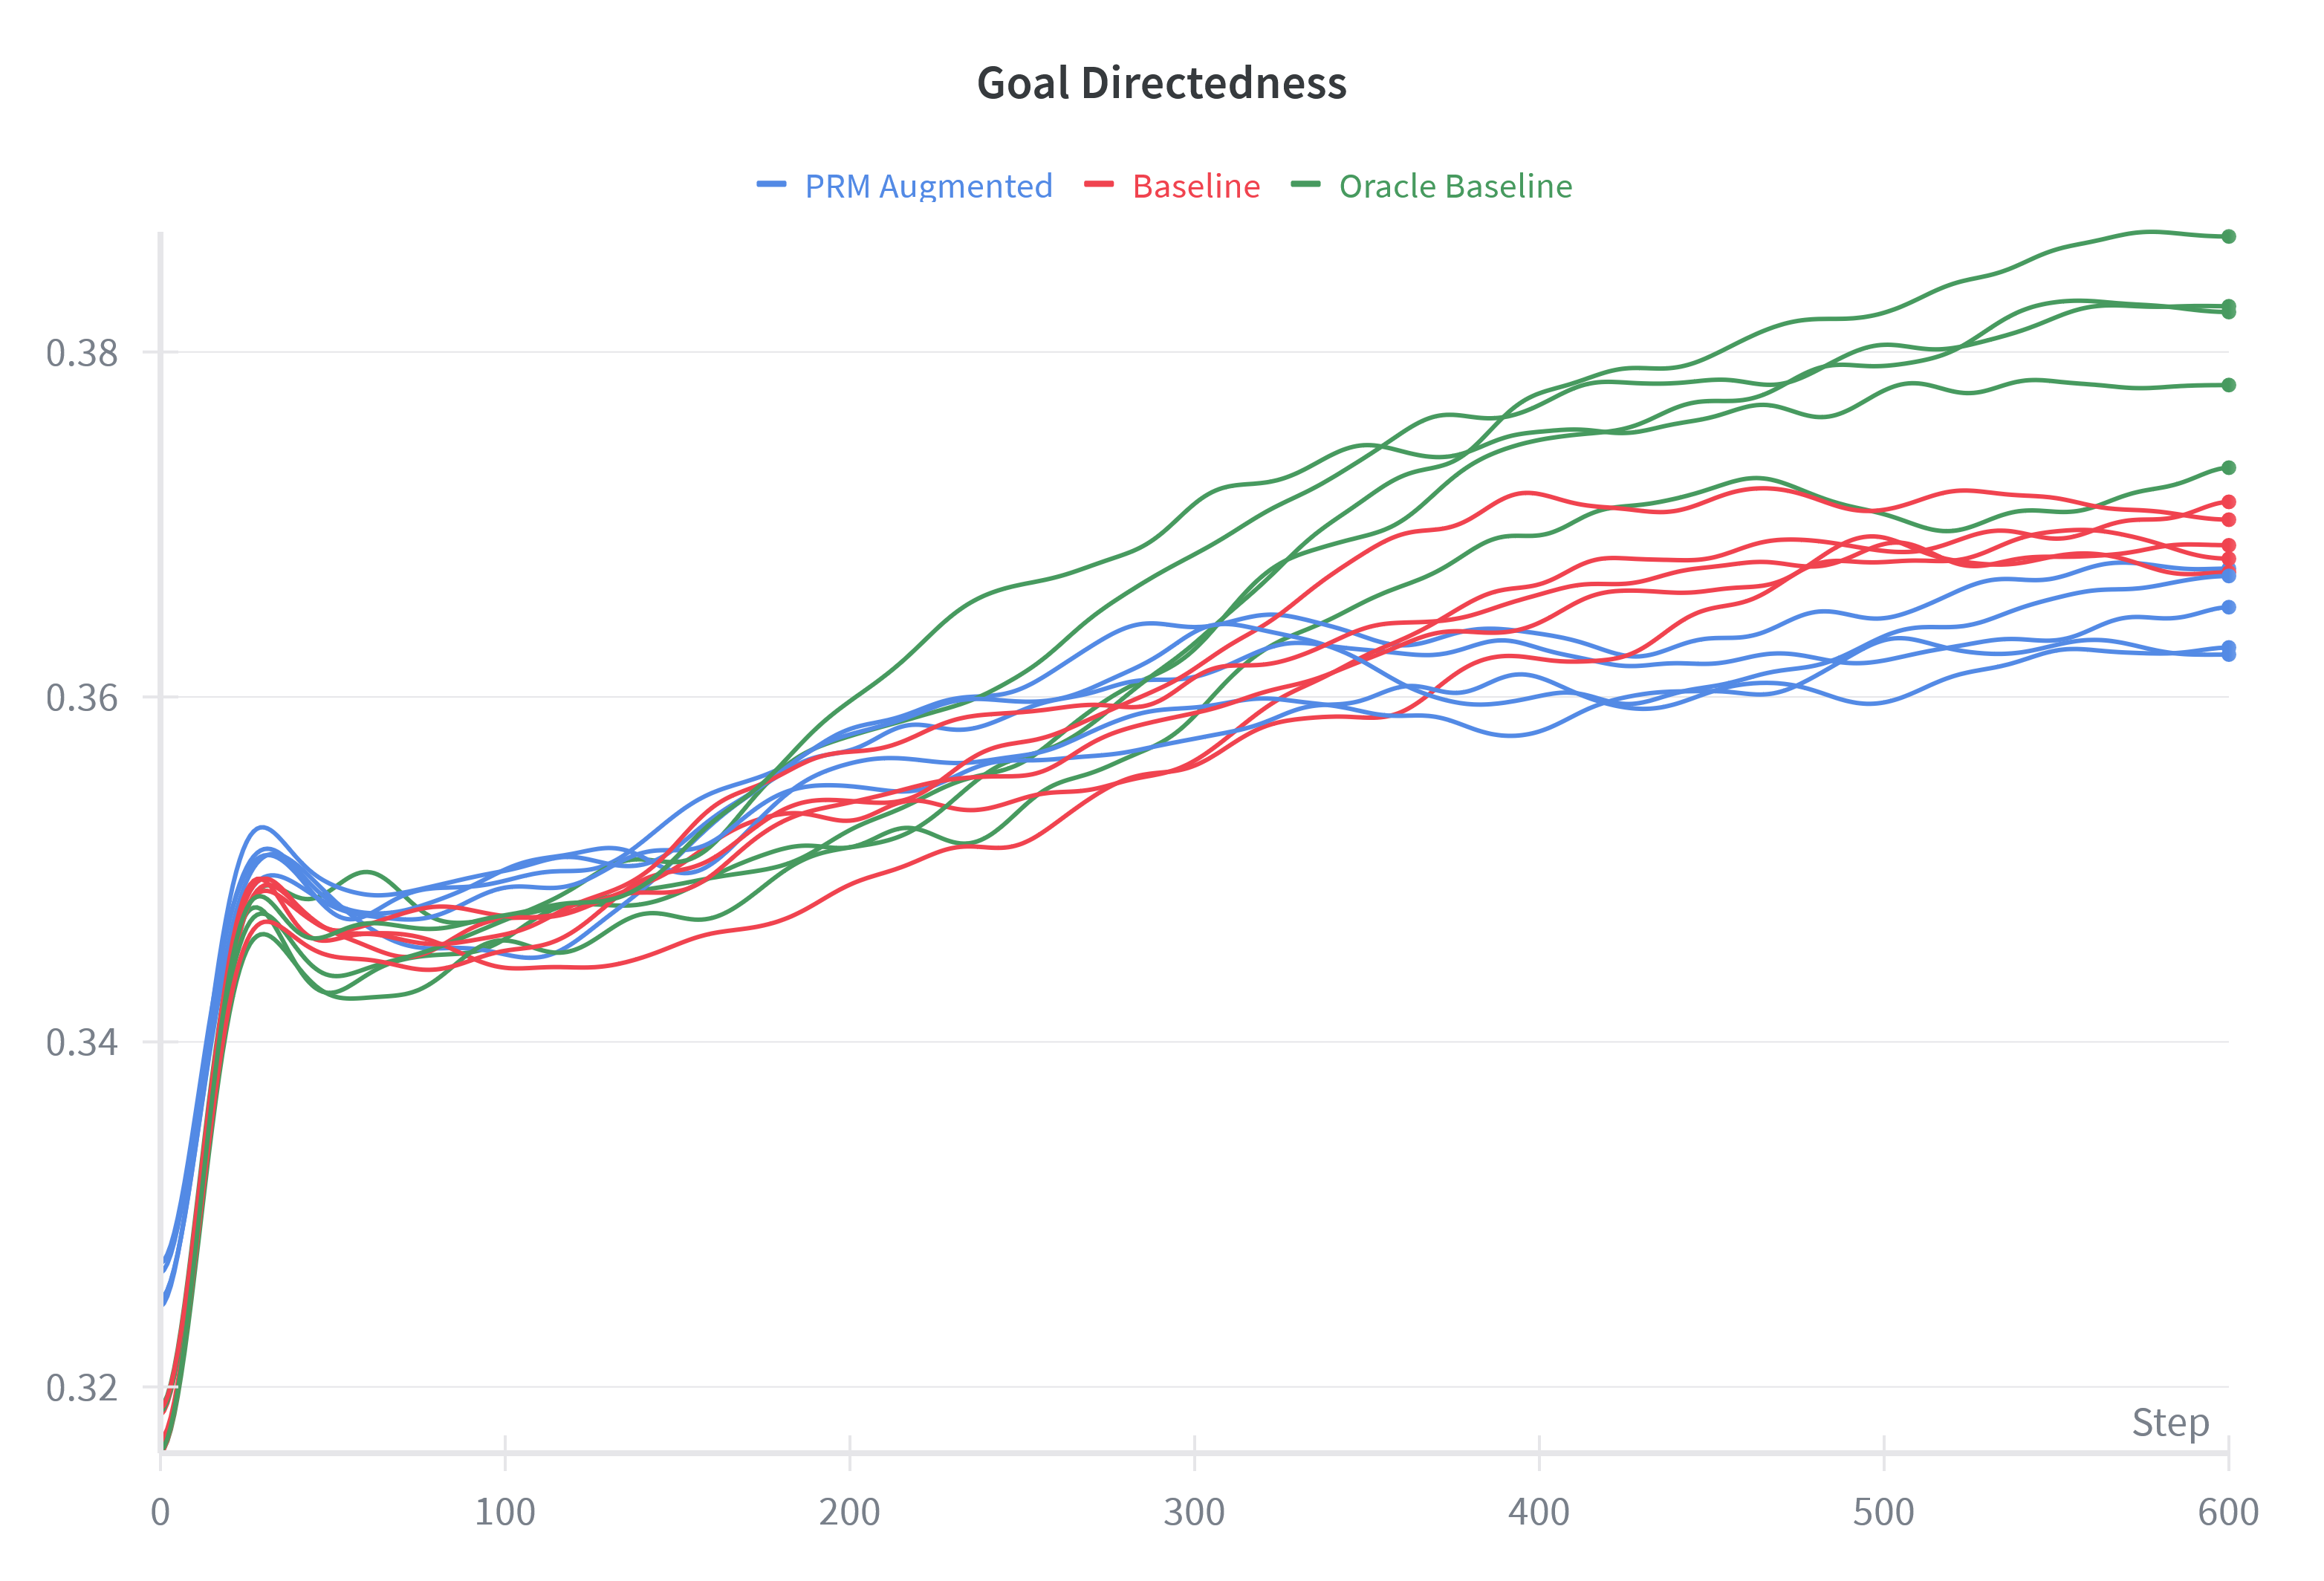
\includegraphics[width=0.8\textwidth]{img/goal_directedness.png}
    \caption{Mean Goal-Directedness over the course of training. The PRM-MASAC model's lower score indicates a policy that systematically deviates from the shortest path to its target, a behavior associated with costly signaling.}
    \label{fig:results_goaldirectedness}
\end{figure}

\paragraph{Action Magnitude}
This "costly signaling" interpretation is further supported by the Team Action Magnitude, shown in Figure \ref{fig:results_magnitude}. The Oracle, with perfect information, can afford to be efficient, resulting in the lowest average action magnitude. The baseline agent requires slightly more effort to navigate its uncertain environment. The PRM-MASAC agent, however, sustains the highest average action magnitude. This suggests that the "signaling moves"—the deviations from the direct path—are "expensive" and require the agent to expend more energy, taking larger or more compensatory actions to execute these legible trajectories while still attempting to complete the task.

\begin{figure}[h!]
    \centering
    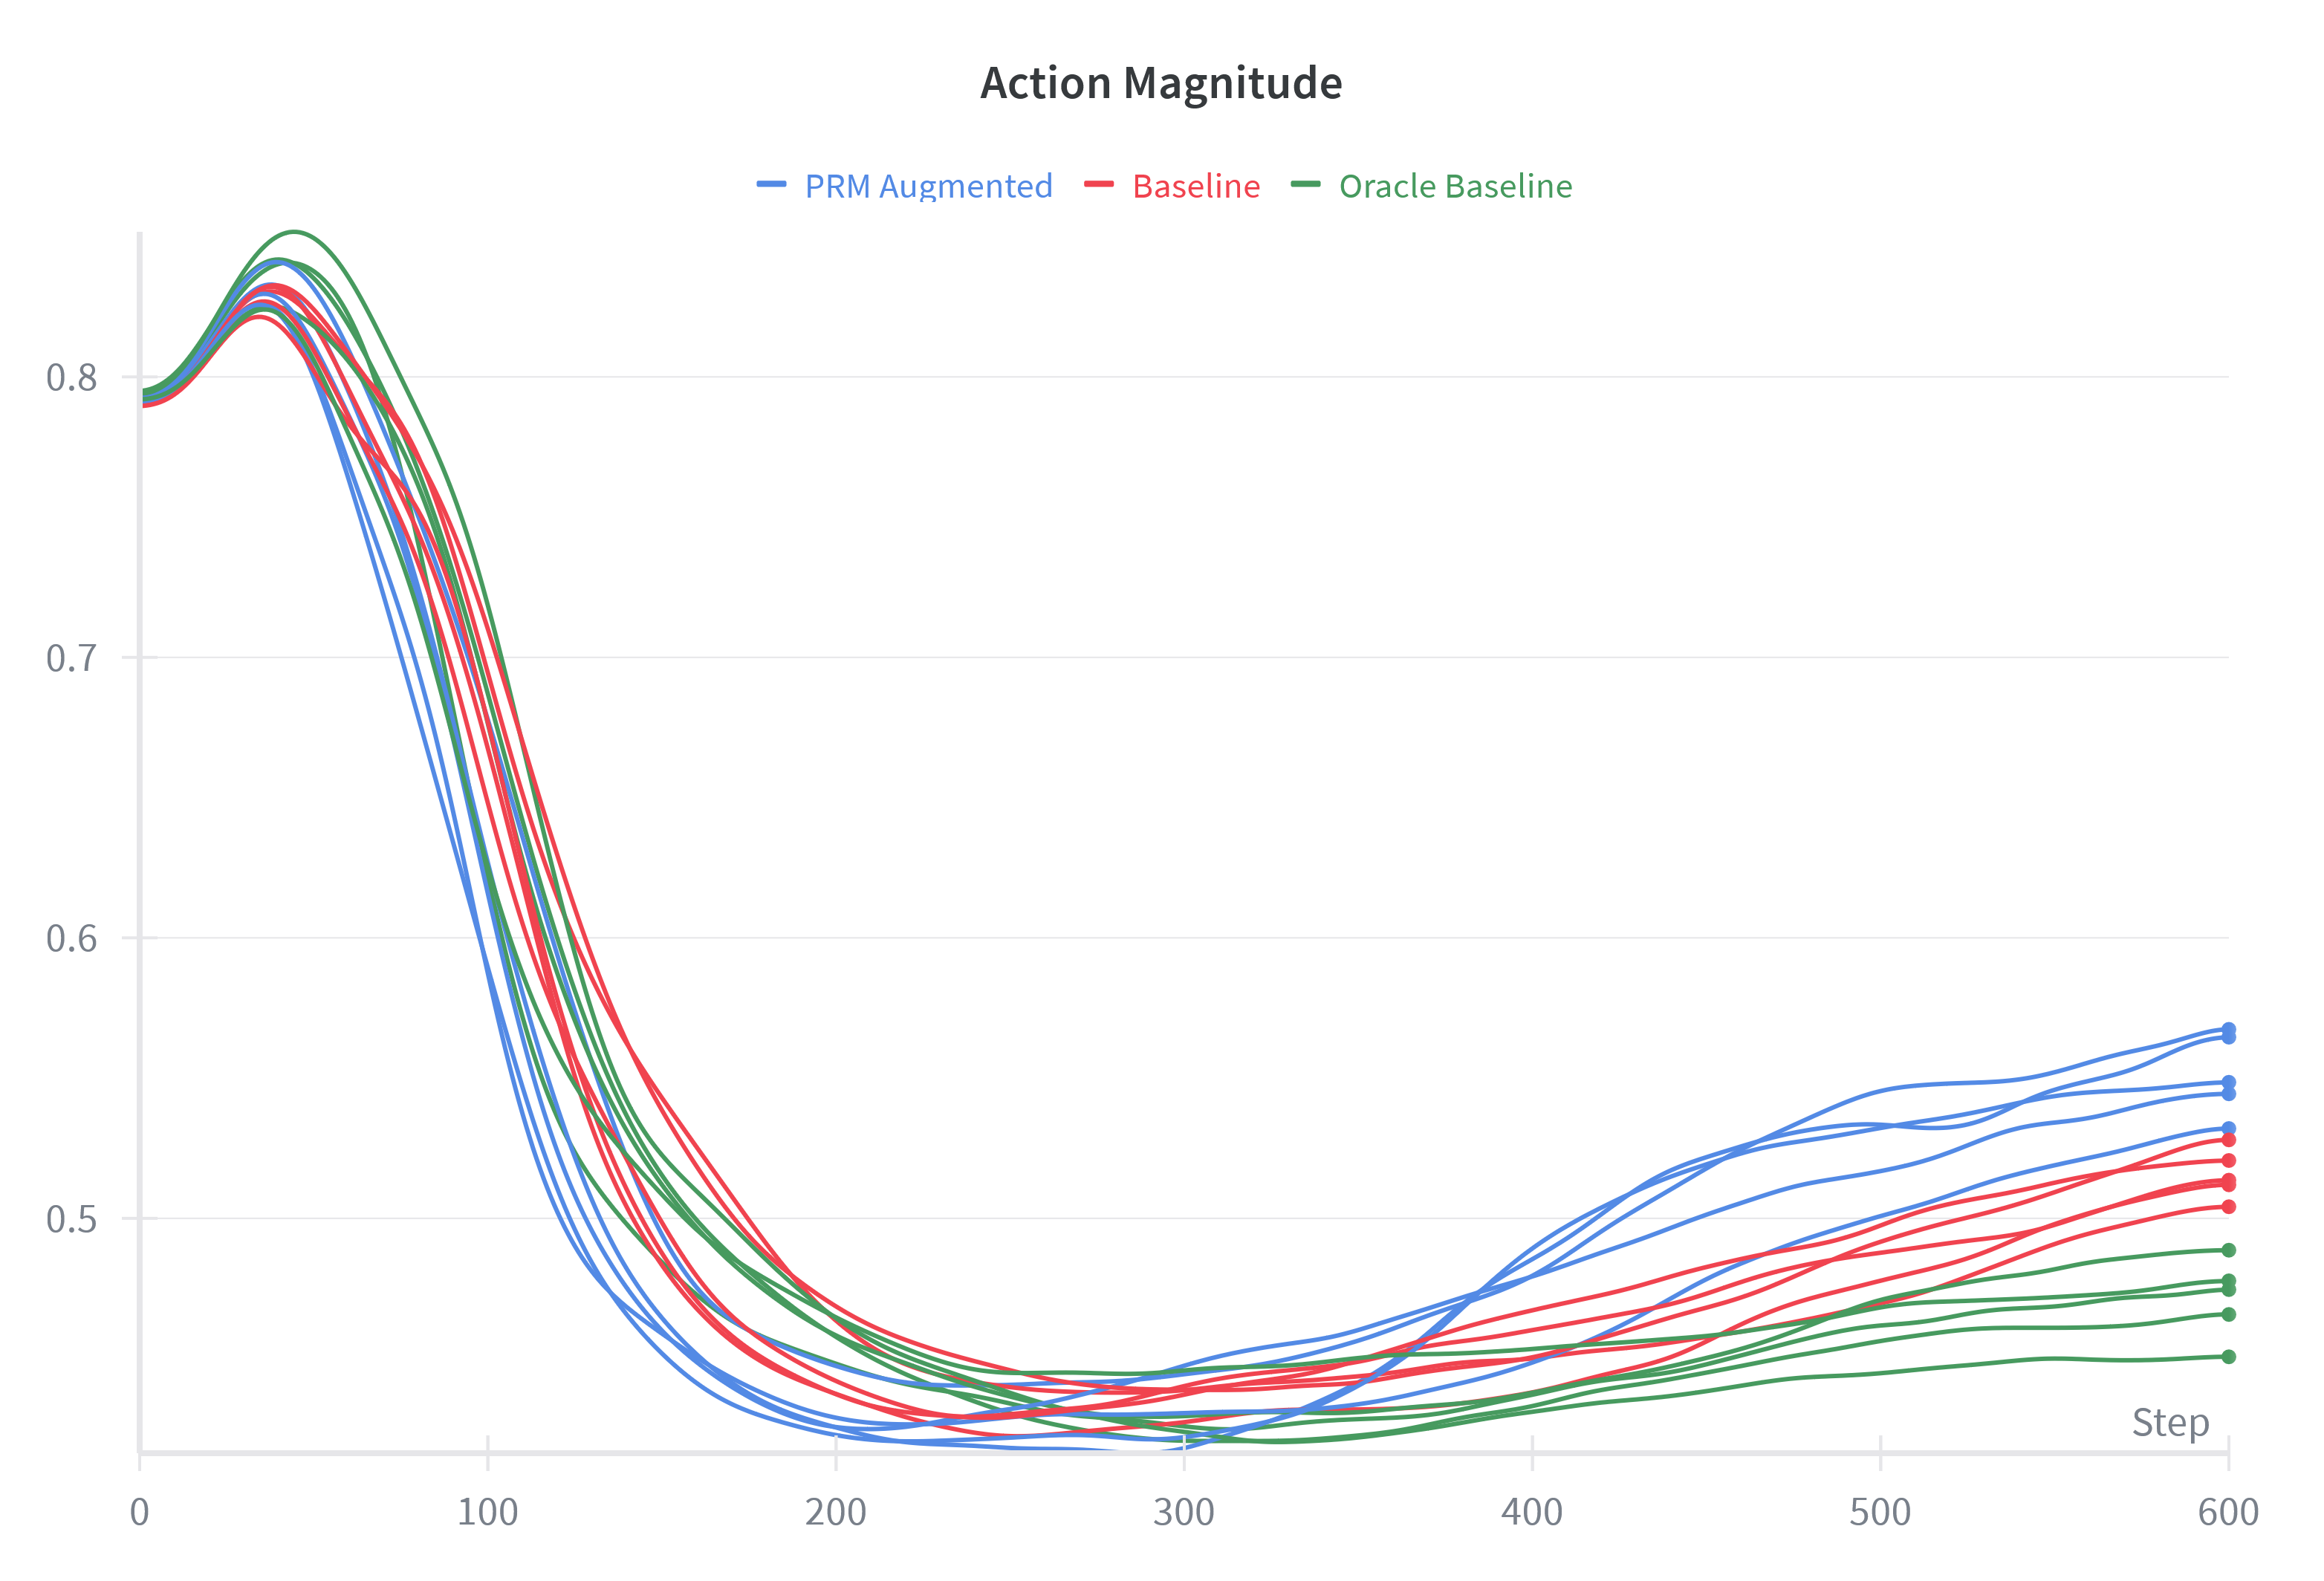
\includegraphics[width=0.8\textwidth]{img/action_magnitude.png}
    \caption{Mean Team Action Magnitude over the course of training. The PRM-MASAC model's need to execute "expensive" signaling moves results in a policy with a consistently higher average action magnitude.}
    \label{fig:results_magnitude}
\end{figure}

\section{Evaluation of Communicative Efficacy}
\label{sec:results_communication}

While behavioral metrics confirm that the PRM agent is \textit{attempting} to signal, we next evaluate whether this signaling is \textit{effective}. The results here present a significant contradiction: the agent fails to optimize the very metrics it is designed to improve.

\paragraph{Communicative Clarity and Reward}

Communicative Clarity, the primary measure of legibility derived from the pragmatic listener $L^*$, shows a surprising result in Figure \ref{fig:results_comm_clarity}. While the Oracle (which has no ambiguity to resolve) demonstrates near-perfect clarity, the PRM agent's clarity score is remarkably similar to the Standard Baseline. This is mirrored in the Communicative Reward (Figure \ref{fig:results_comm_reward}), which is the raw reward signal $\Rcomm$. The PRM-MASAC agent appears unable to directly optimize this reward, performing no better than the baseline. This suggests that while the agent learns to execute costly behaviors (low goal-directedness, high magnitude), these actions are \textit{not} successfully interpreted as "clear" by the pragmatic listener model.

\begin{figure}[h!]
    \centering
    \begin{minipage}{0.49\textwidth}
        \centering
        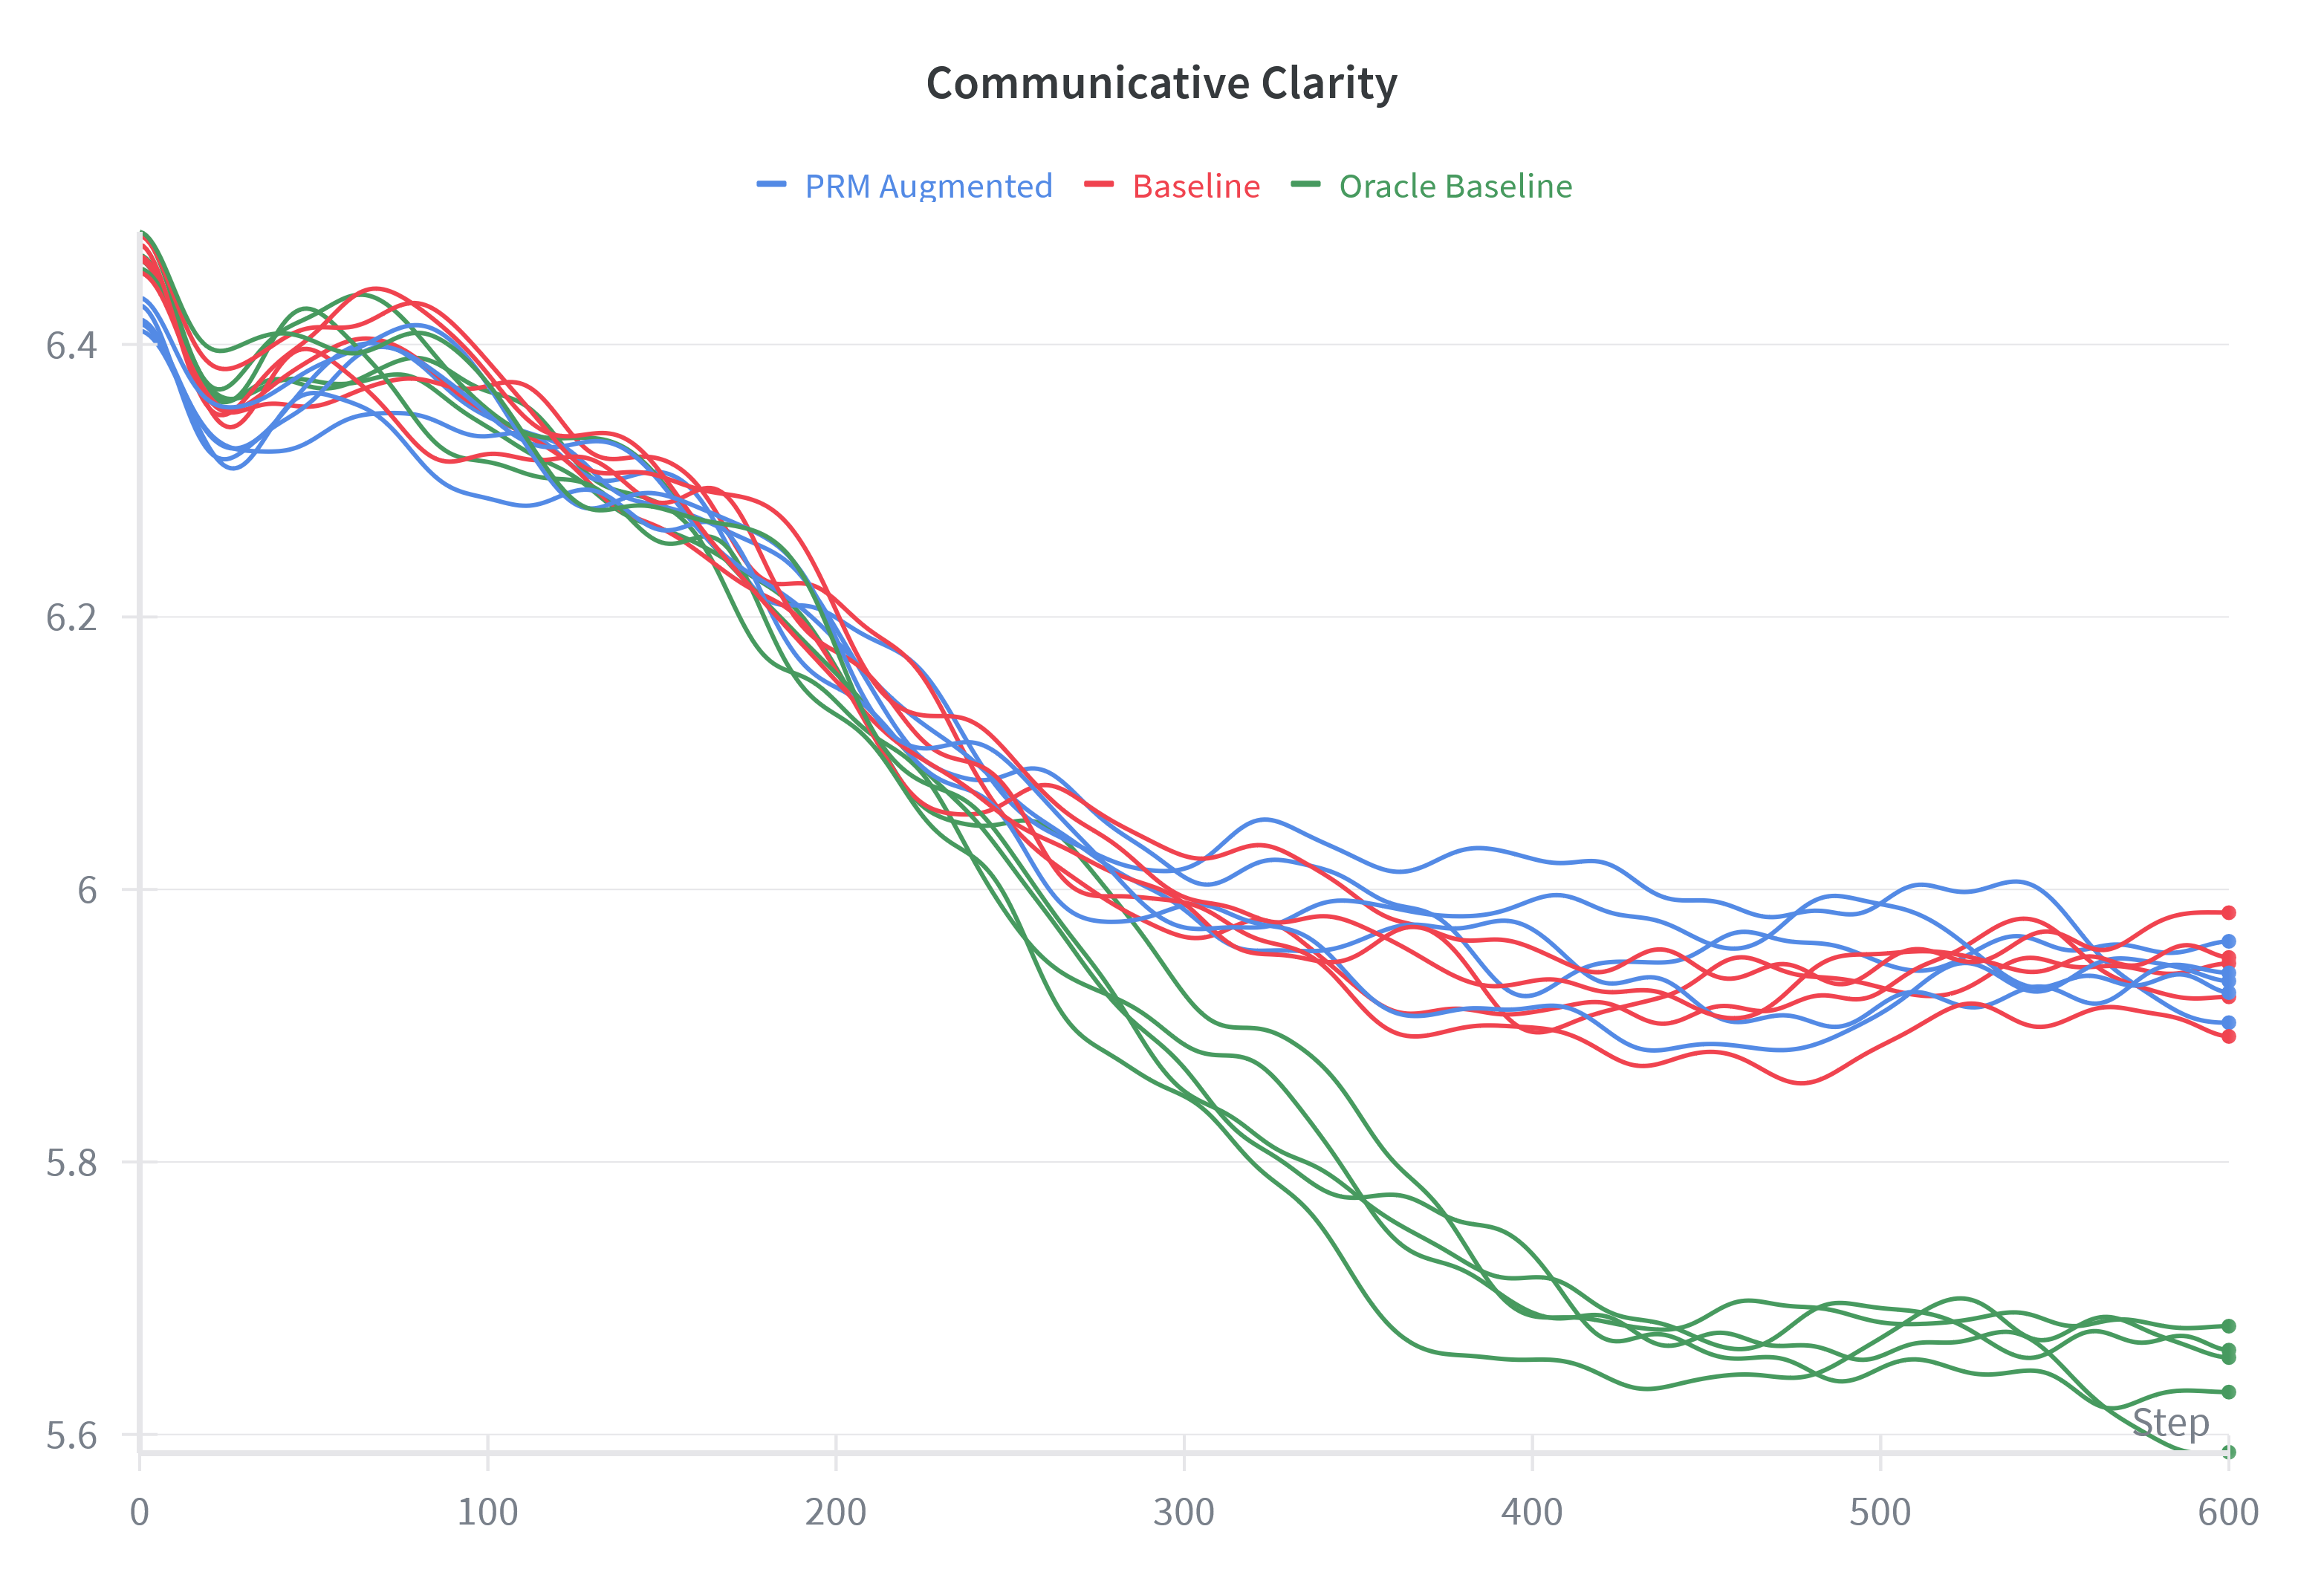
\includegraphics[width=\linewidth]{img/comm_clarity.png}
        \caption{Mean Communicative Clarity. Lower is better. PRM and Baseline are indistinguishable, indicating a failure to produce pragmatically clear actions.}
        \label{fig:results_comm_clarity}
    \end{minipage}\hfill
    \begin{minipage}{0.49\textwidth}
        \centering
        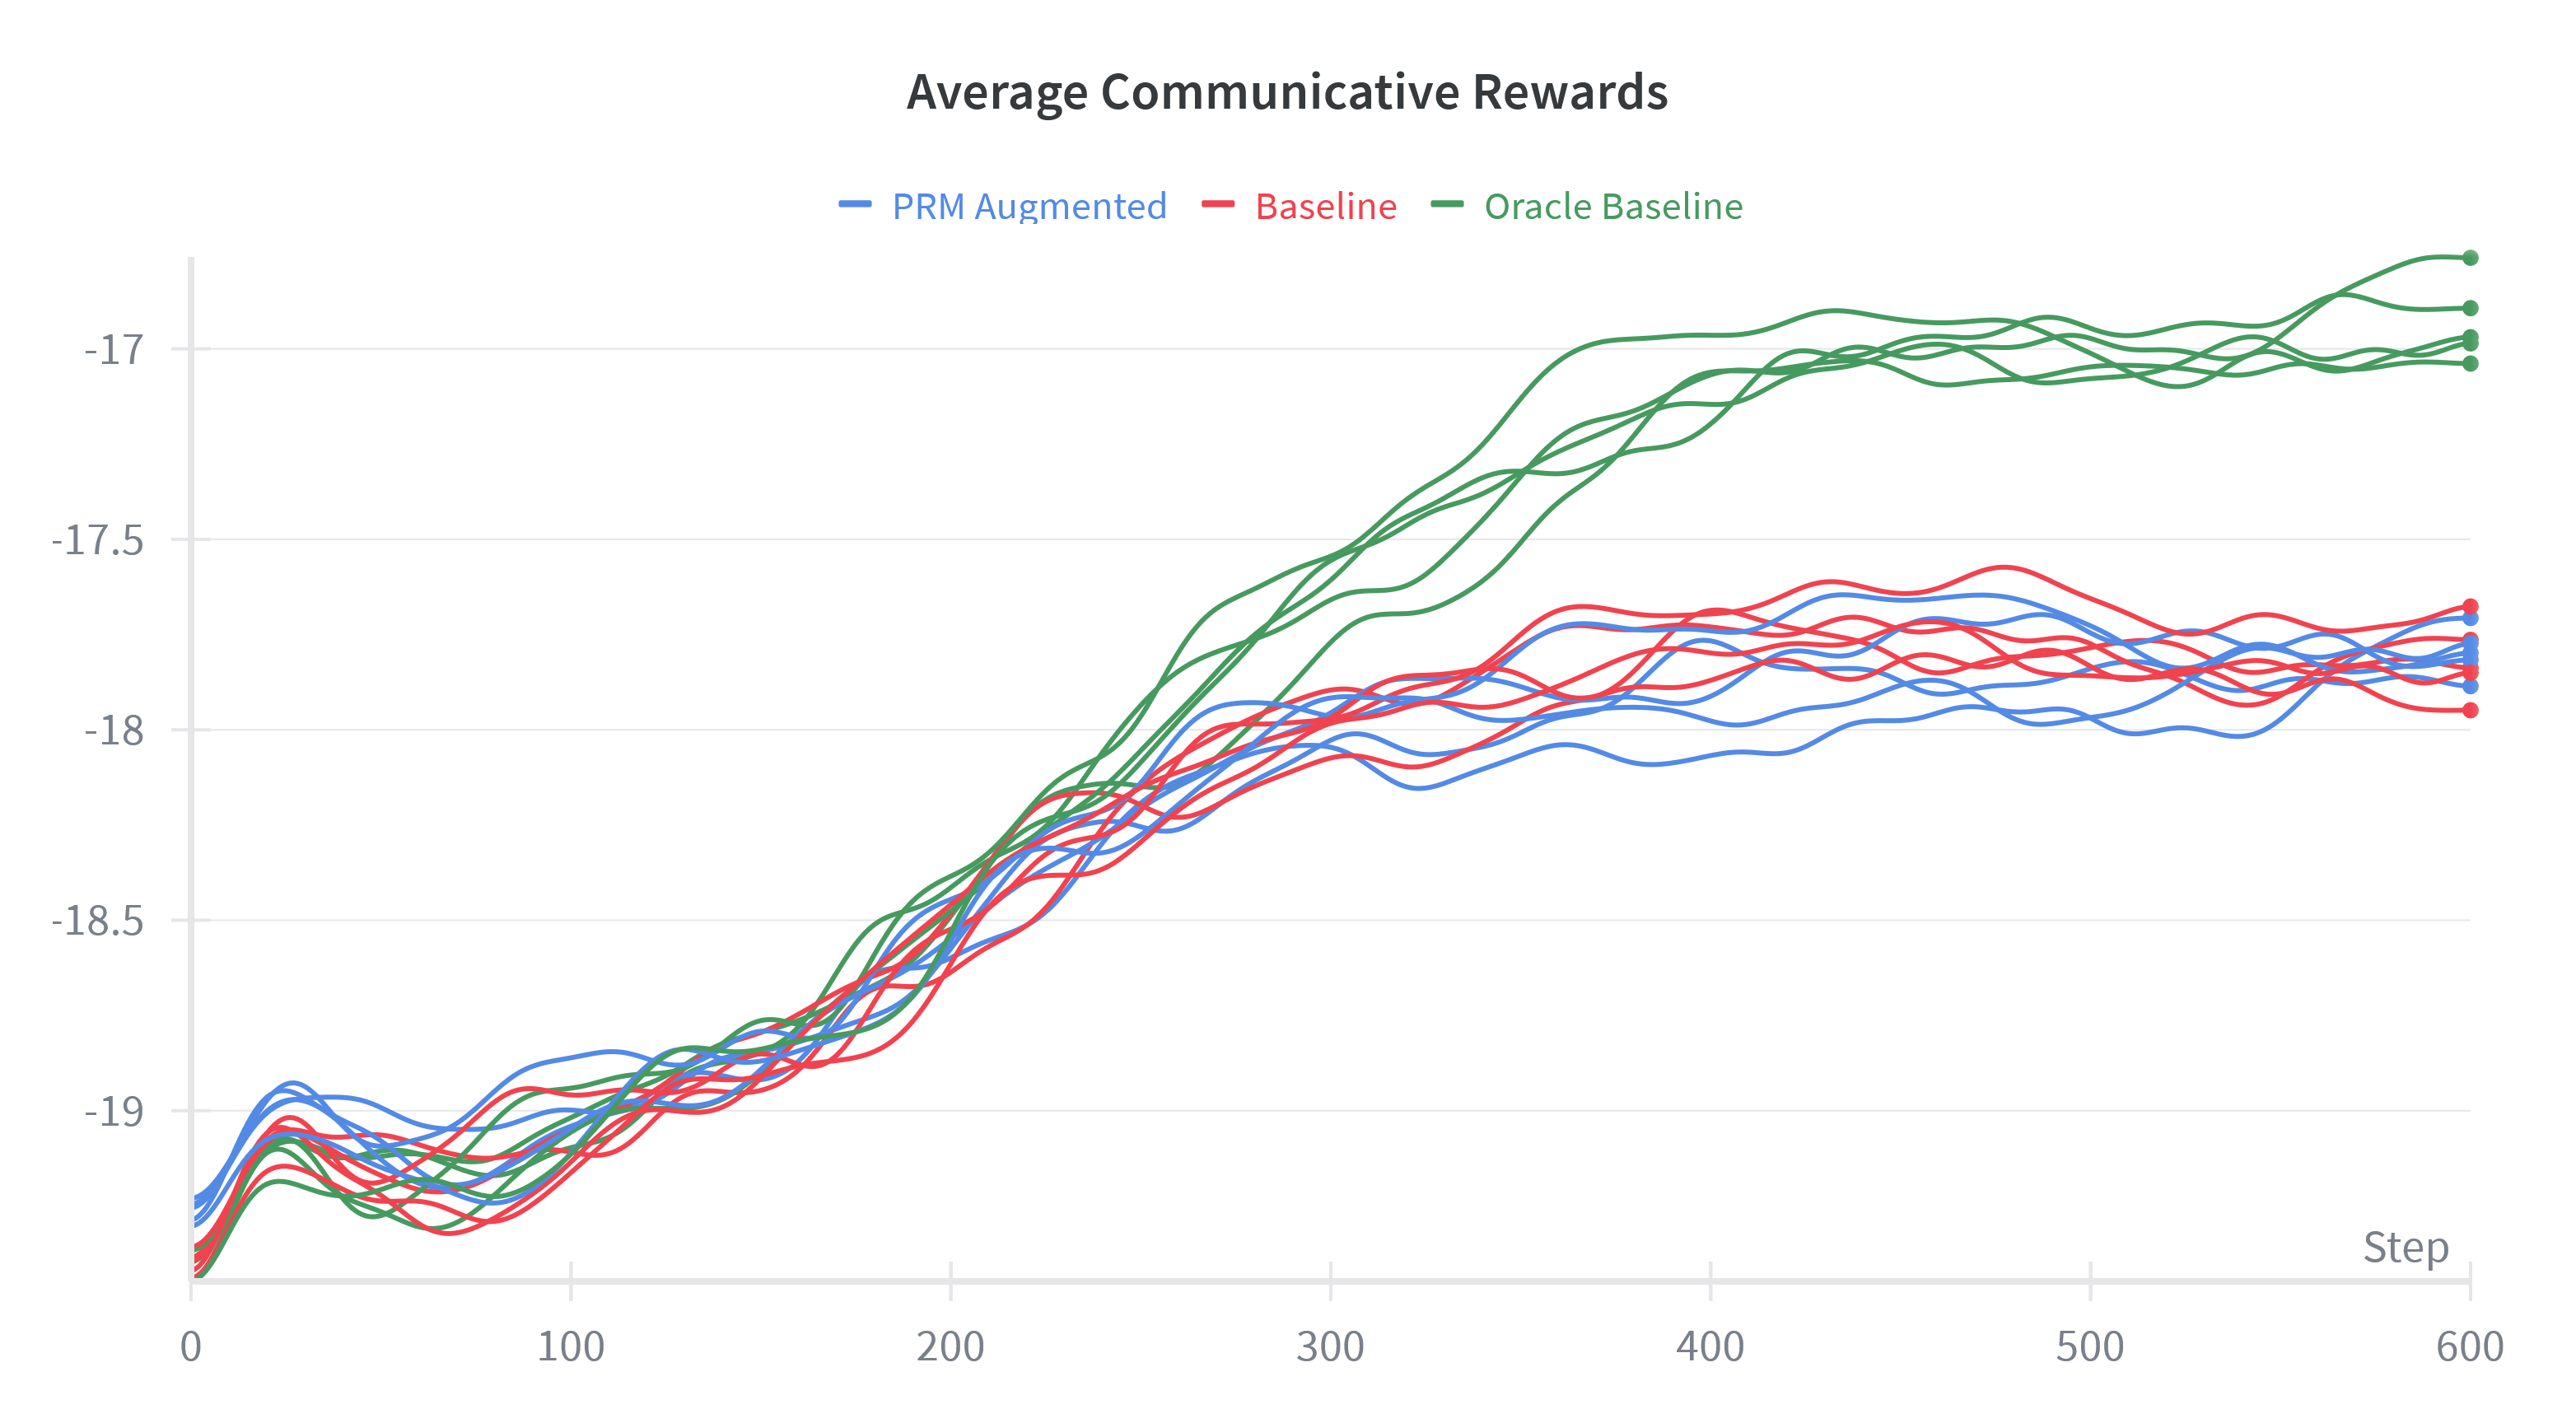
\includegraphics[width=\linewidth]{img/avg_comm_rw.png}
        \caption{Mean Communicative Reward ($\Rcomm$). The PRM agent fails to optimize its intrinsic reward, performing on par with the Baseline.}
        \label{fig:results_comm_reward}
    \end{minipage}
\end{figure}

\paragraph{Literal Intent Accuracy}
This pragmatic failure is contrasted by the Literal Intent Accuracy, which measures the accuracy of the "naive" $L_0$ listener. As seen in Figure \ref{fig:results_intent_accuracy}, all three models perform similarly and at a relatively high level. This indicates that all agents, including the baseline, are generally "pointing" in the correct literal direction. The failure of the PRM agent is therefore not at the literal level, but at the \textit{pragmatic} level: its additional, costly signaling fails to add any measurable clarity beyond what the simple baseline's literal movements already provide. 



\begin{figure}[h!]
    \centering
    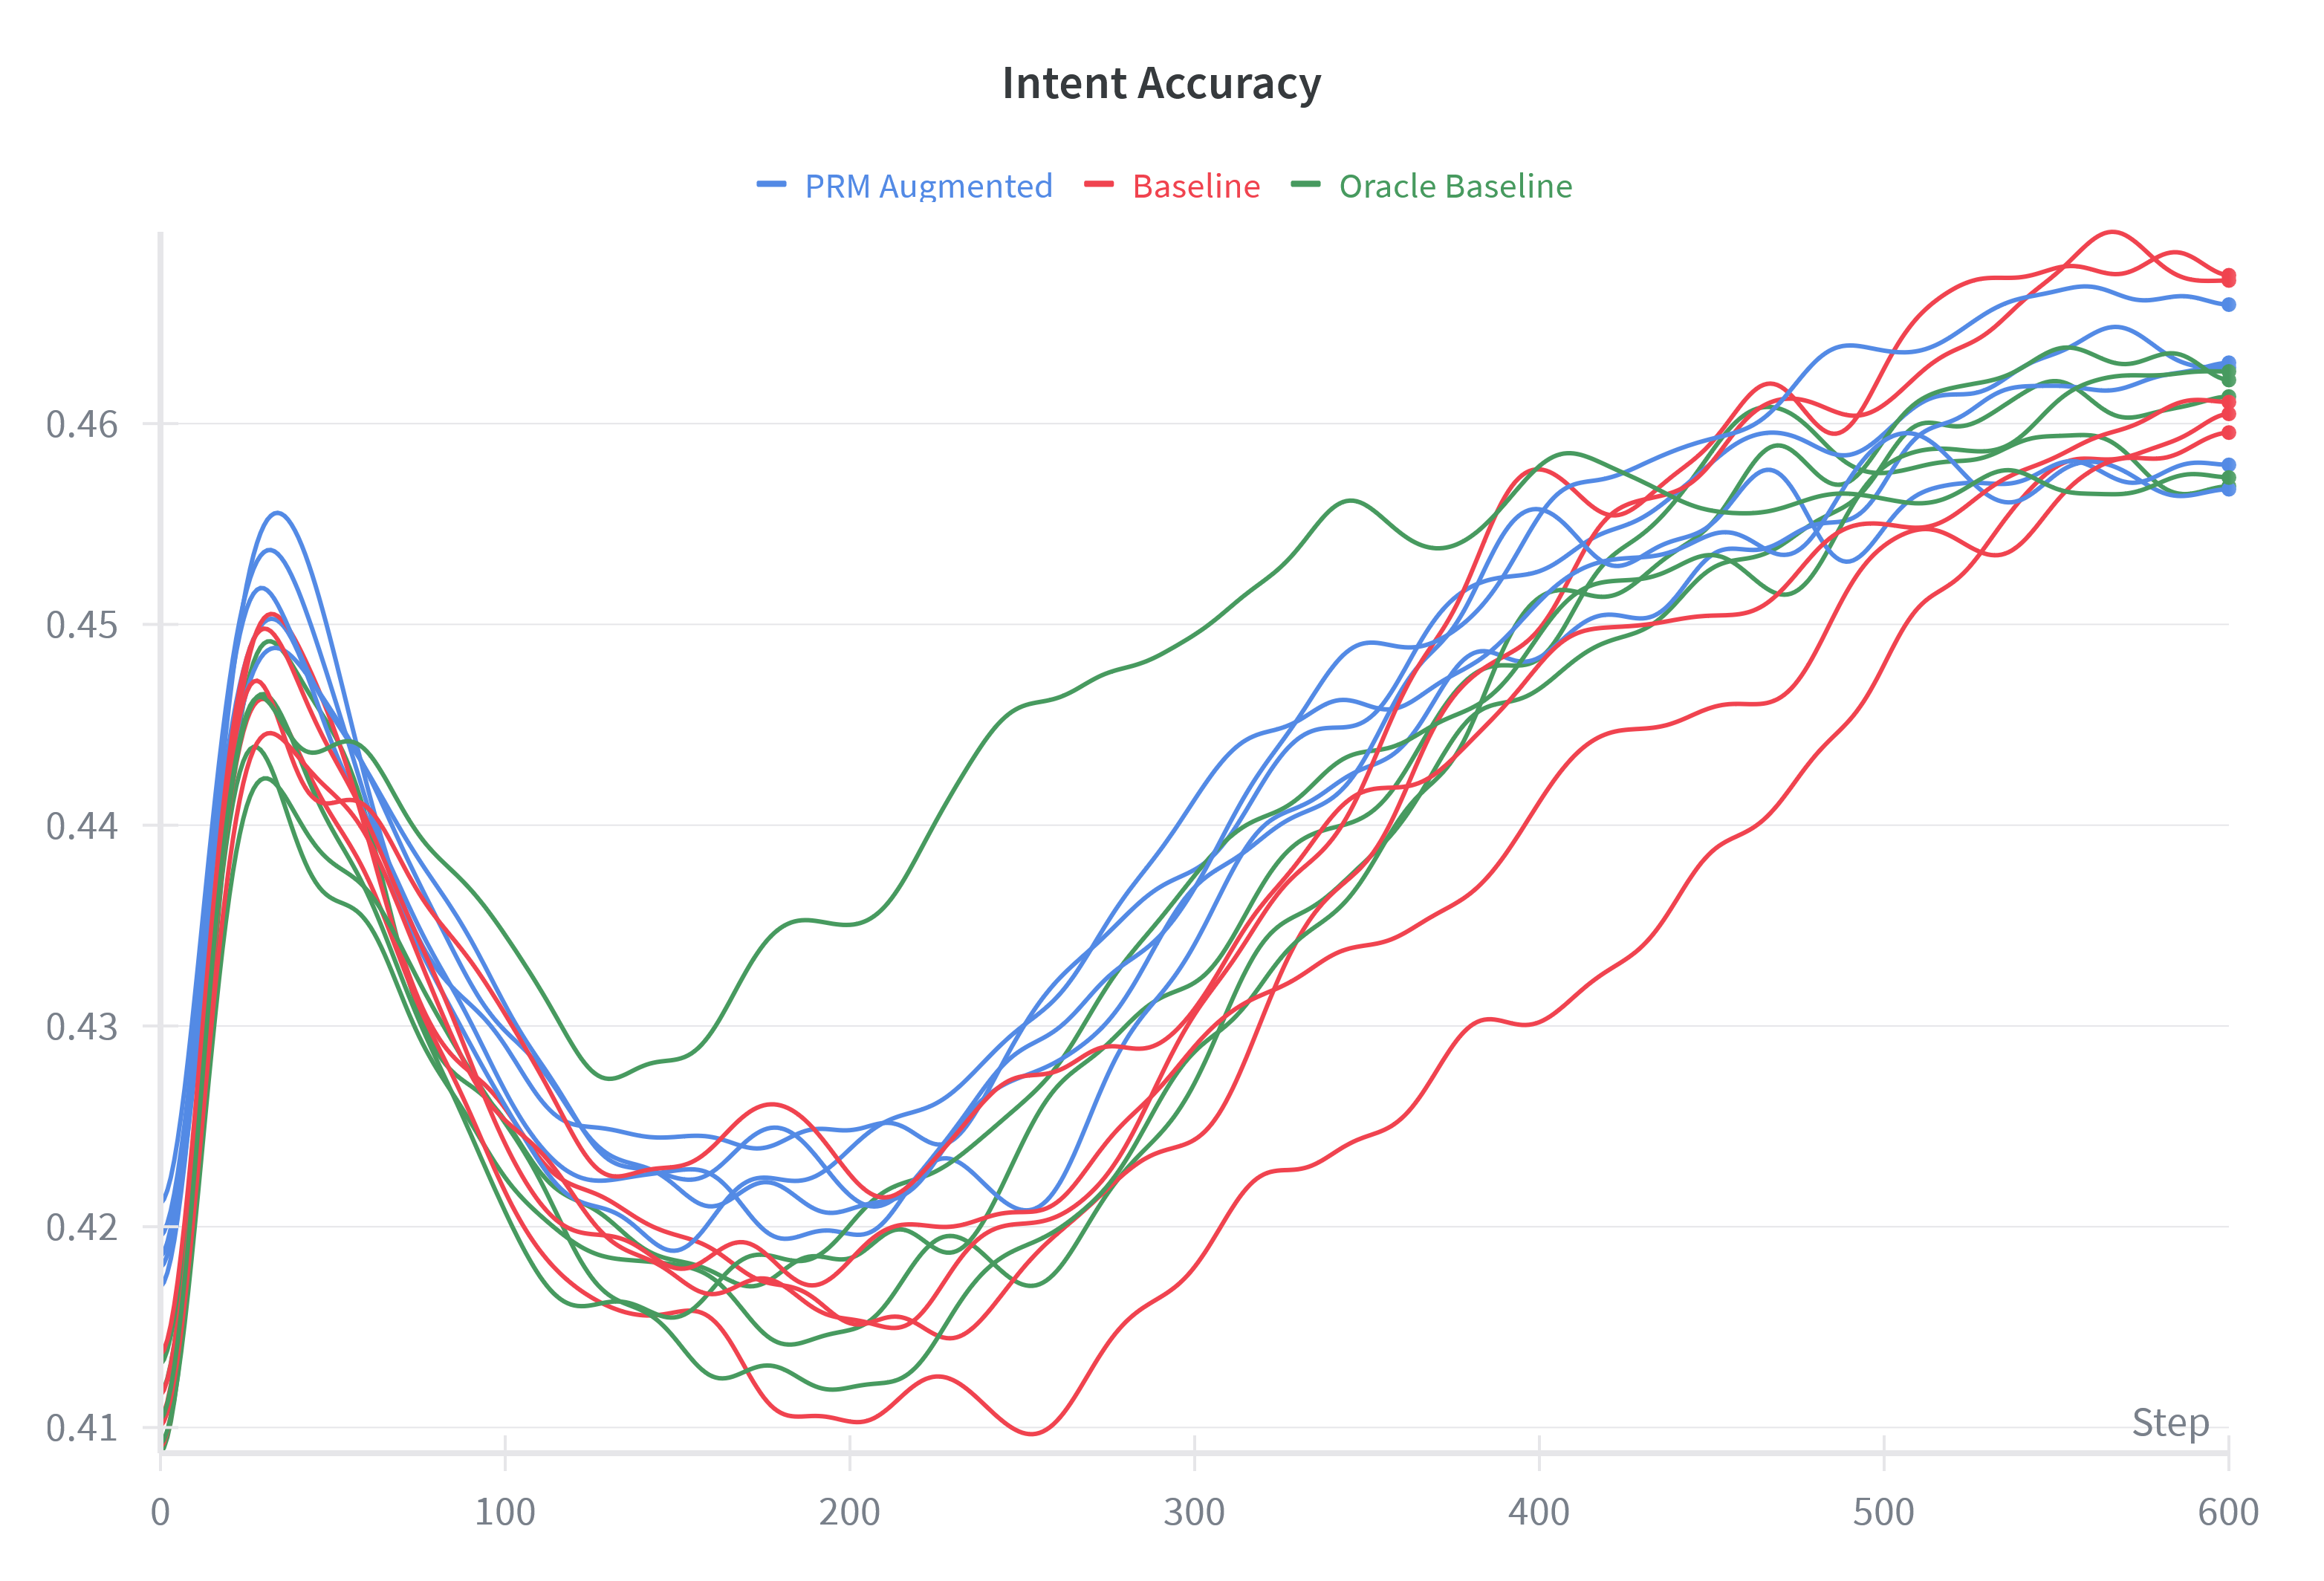
\includegraphics[width=0.8\textwidth]{img/intent_accuracy.png}
    \caption{Literal Intent Accuracy (L0). All three models perform similarly, suggesting the ambiguity in the environment is not solvable by simple literal interpretation alone.}
    \label{fig:results_intent_accuracy}
\end{figure}

\section{Impact on Team Coordination and Task Performance}
\label{sec:results_performance}

Given that the PRM agent's signaling is costly but communicatively ineffective, we analyze its impact on task-level coordination and reward. The results show that the PRM agent's strategy fails to translate into a meaningful performance gain.

\paragraph{Team Specialization}
The primary goal of coordination in this task is division of labor, measured by Team Specialization. Figure \ref{fig:results_specialization} shows the most critical failure: the PRM-augmented agent achieves no significant improvement in specialization over the Standard Baseline. Both models fail to divide labor effectively. Only the Oracle, with its perfect information, achieves a high specialization score. This confirms that the PRM's signaling behavior does not successfully solve the core coordination problem.

\begin{figure}[h!]
    \centering
    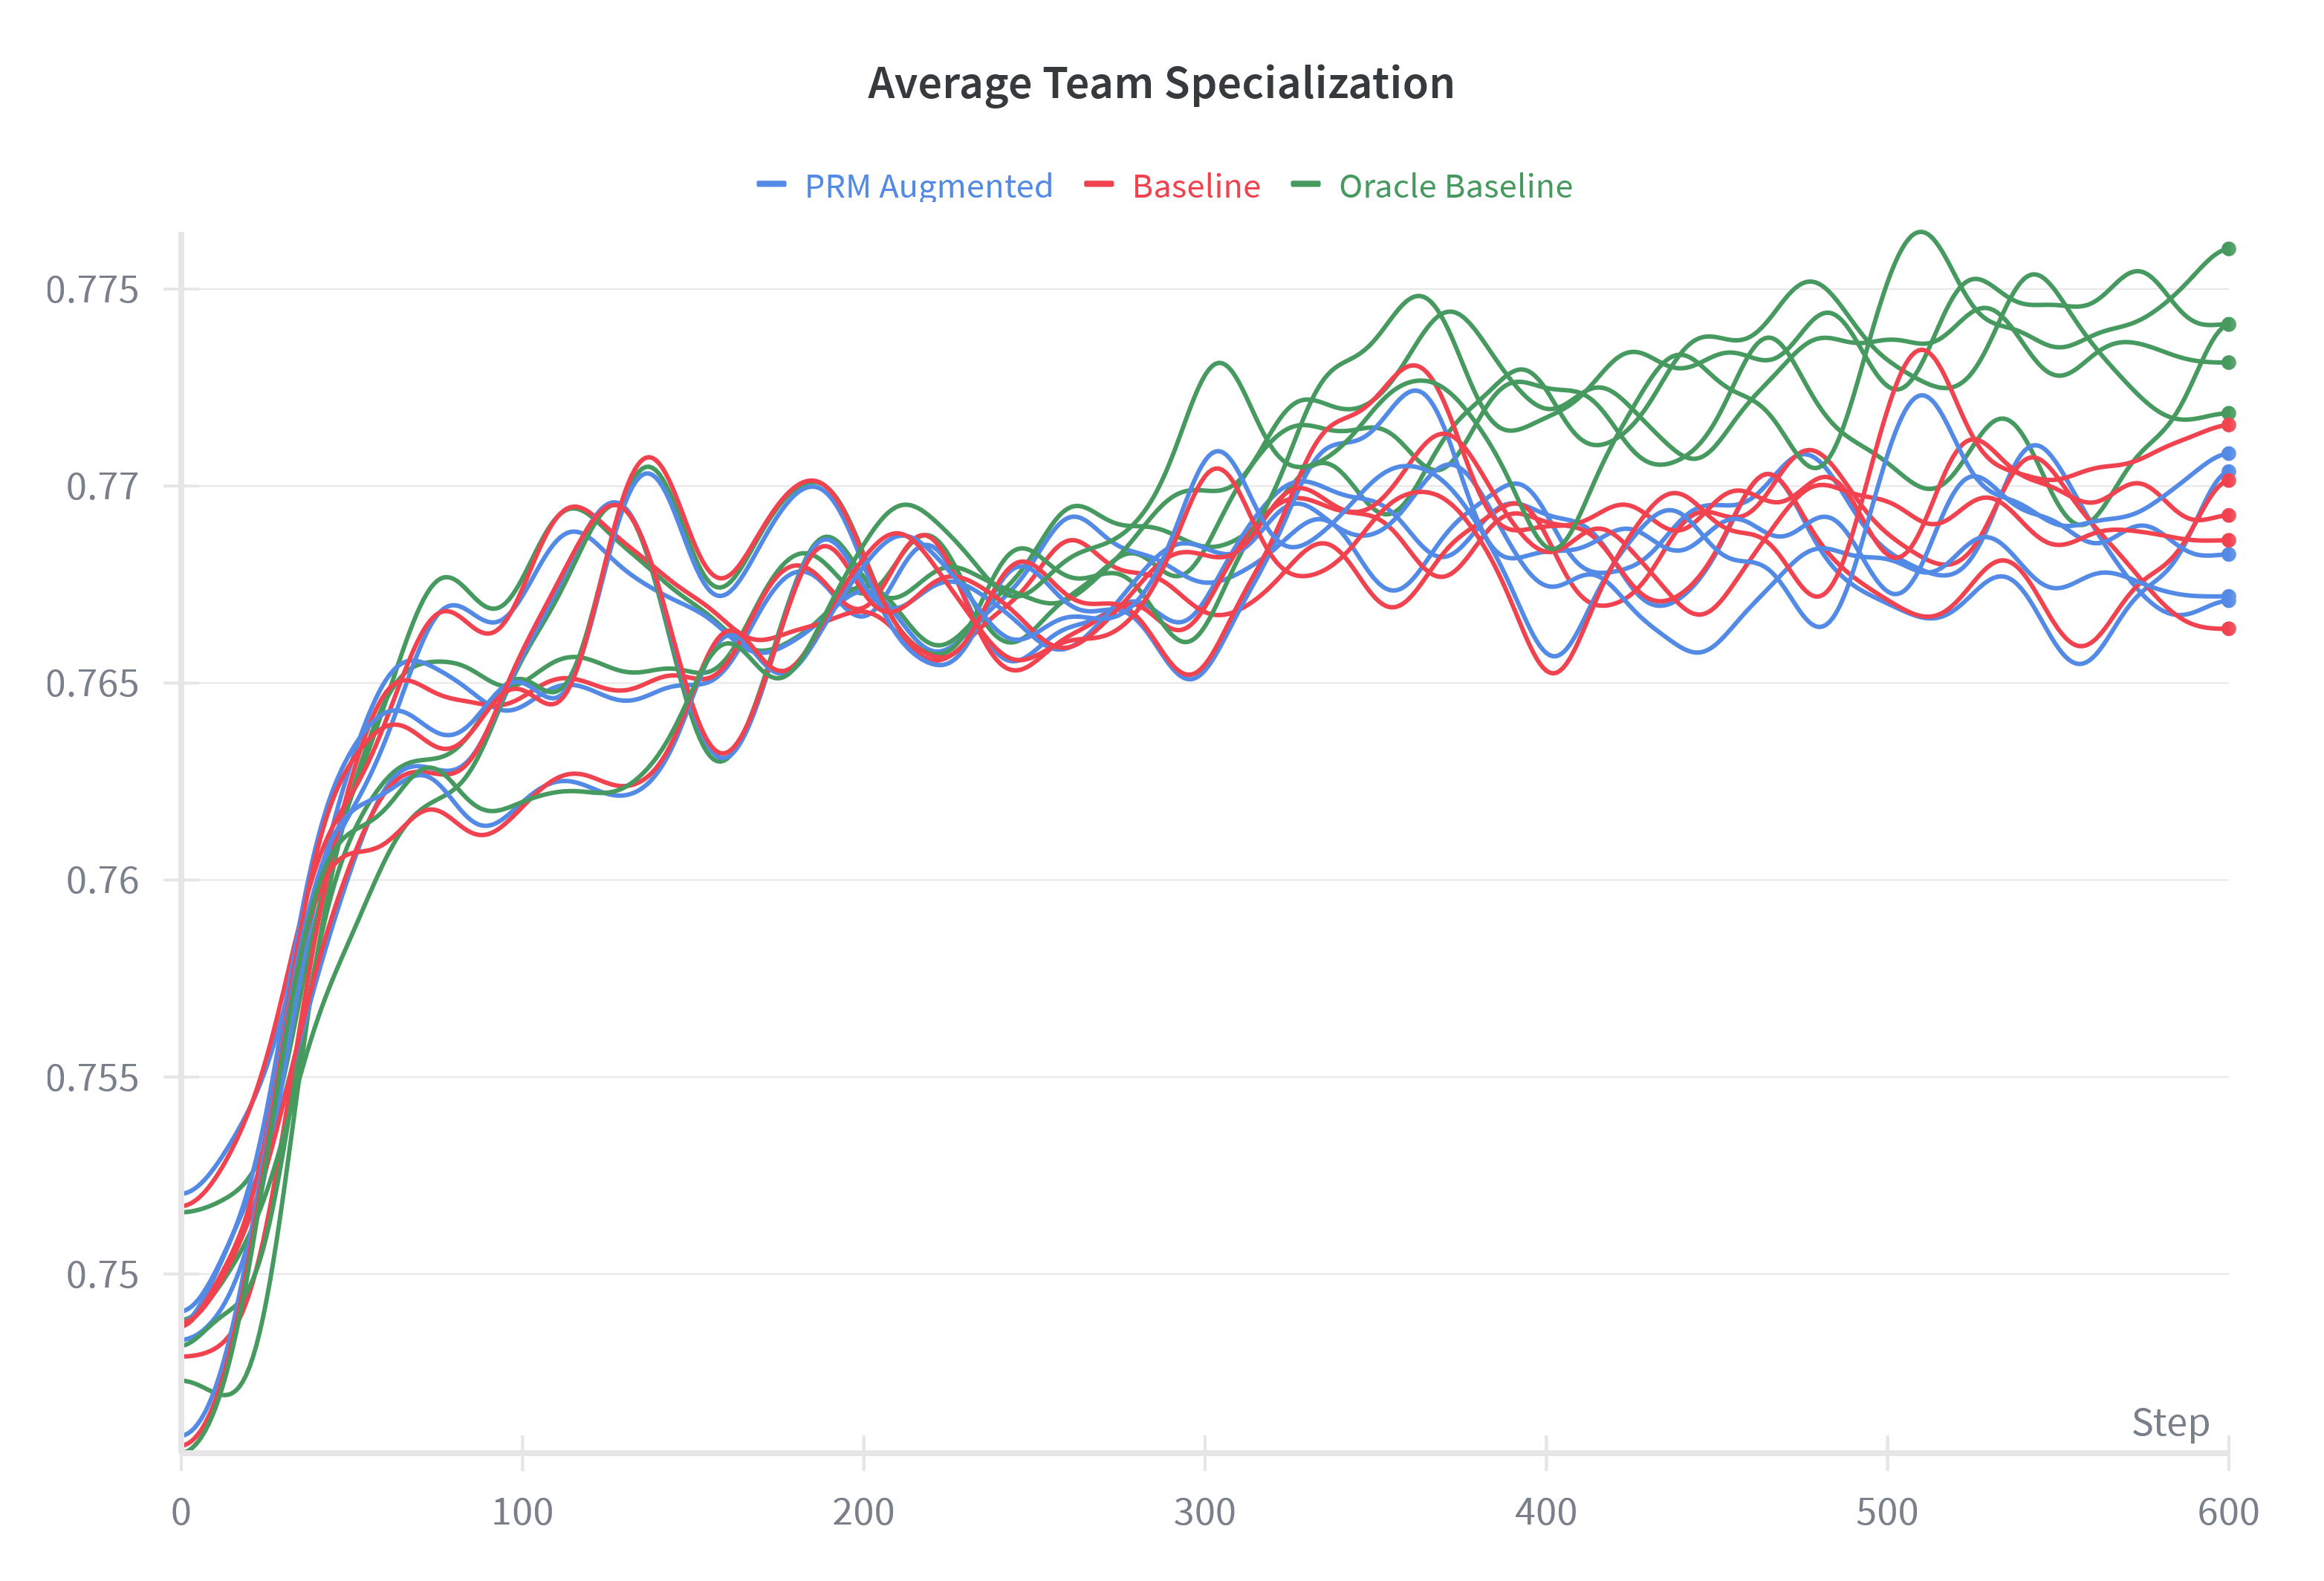
\includegraphics[width=0.8\textwidth]{img/team_spec.png}
    \caption{Mean Team Specialization. The PRM agent's signaling fails to produce better division of labor, as its specialization rate is nearly identical to the Baseline.}
    \label{fig:results_specialization}
\end{figure}

\paragraph{Task Reward Components}
This lack of coordination is reflected in the final task rewards. The Preference Bonus (Figure \ref{fig:results_pref_bonus}), awarded for covering the correct landmarks, is only marginally better for PRM-MASAC than for the baseline. This slight gain is offset by the Team Distance and Collision Penalties (Figure \ref{fig:results_penalties}). The Standard Baseline, by "focusing" naïvely on minimizing distance, achieves the lowest penalties. The PRM-MASAC agent's more complex and higher-magnitude signaling strategy, however, incurs slightly \textit{higher} penalties. The net effect is that the PRM-MASAC agent's costly and communicatively-ineffective strategy yields almost no tangible benefit in overall task performance.

\begin{figure}[h!]
    \centering
    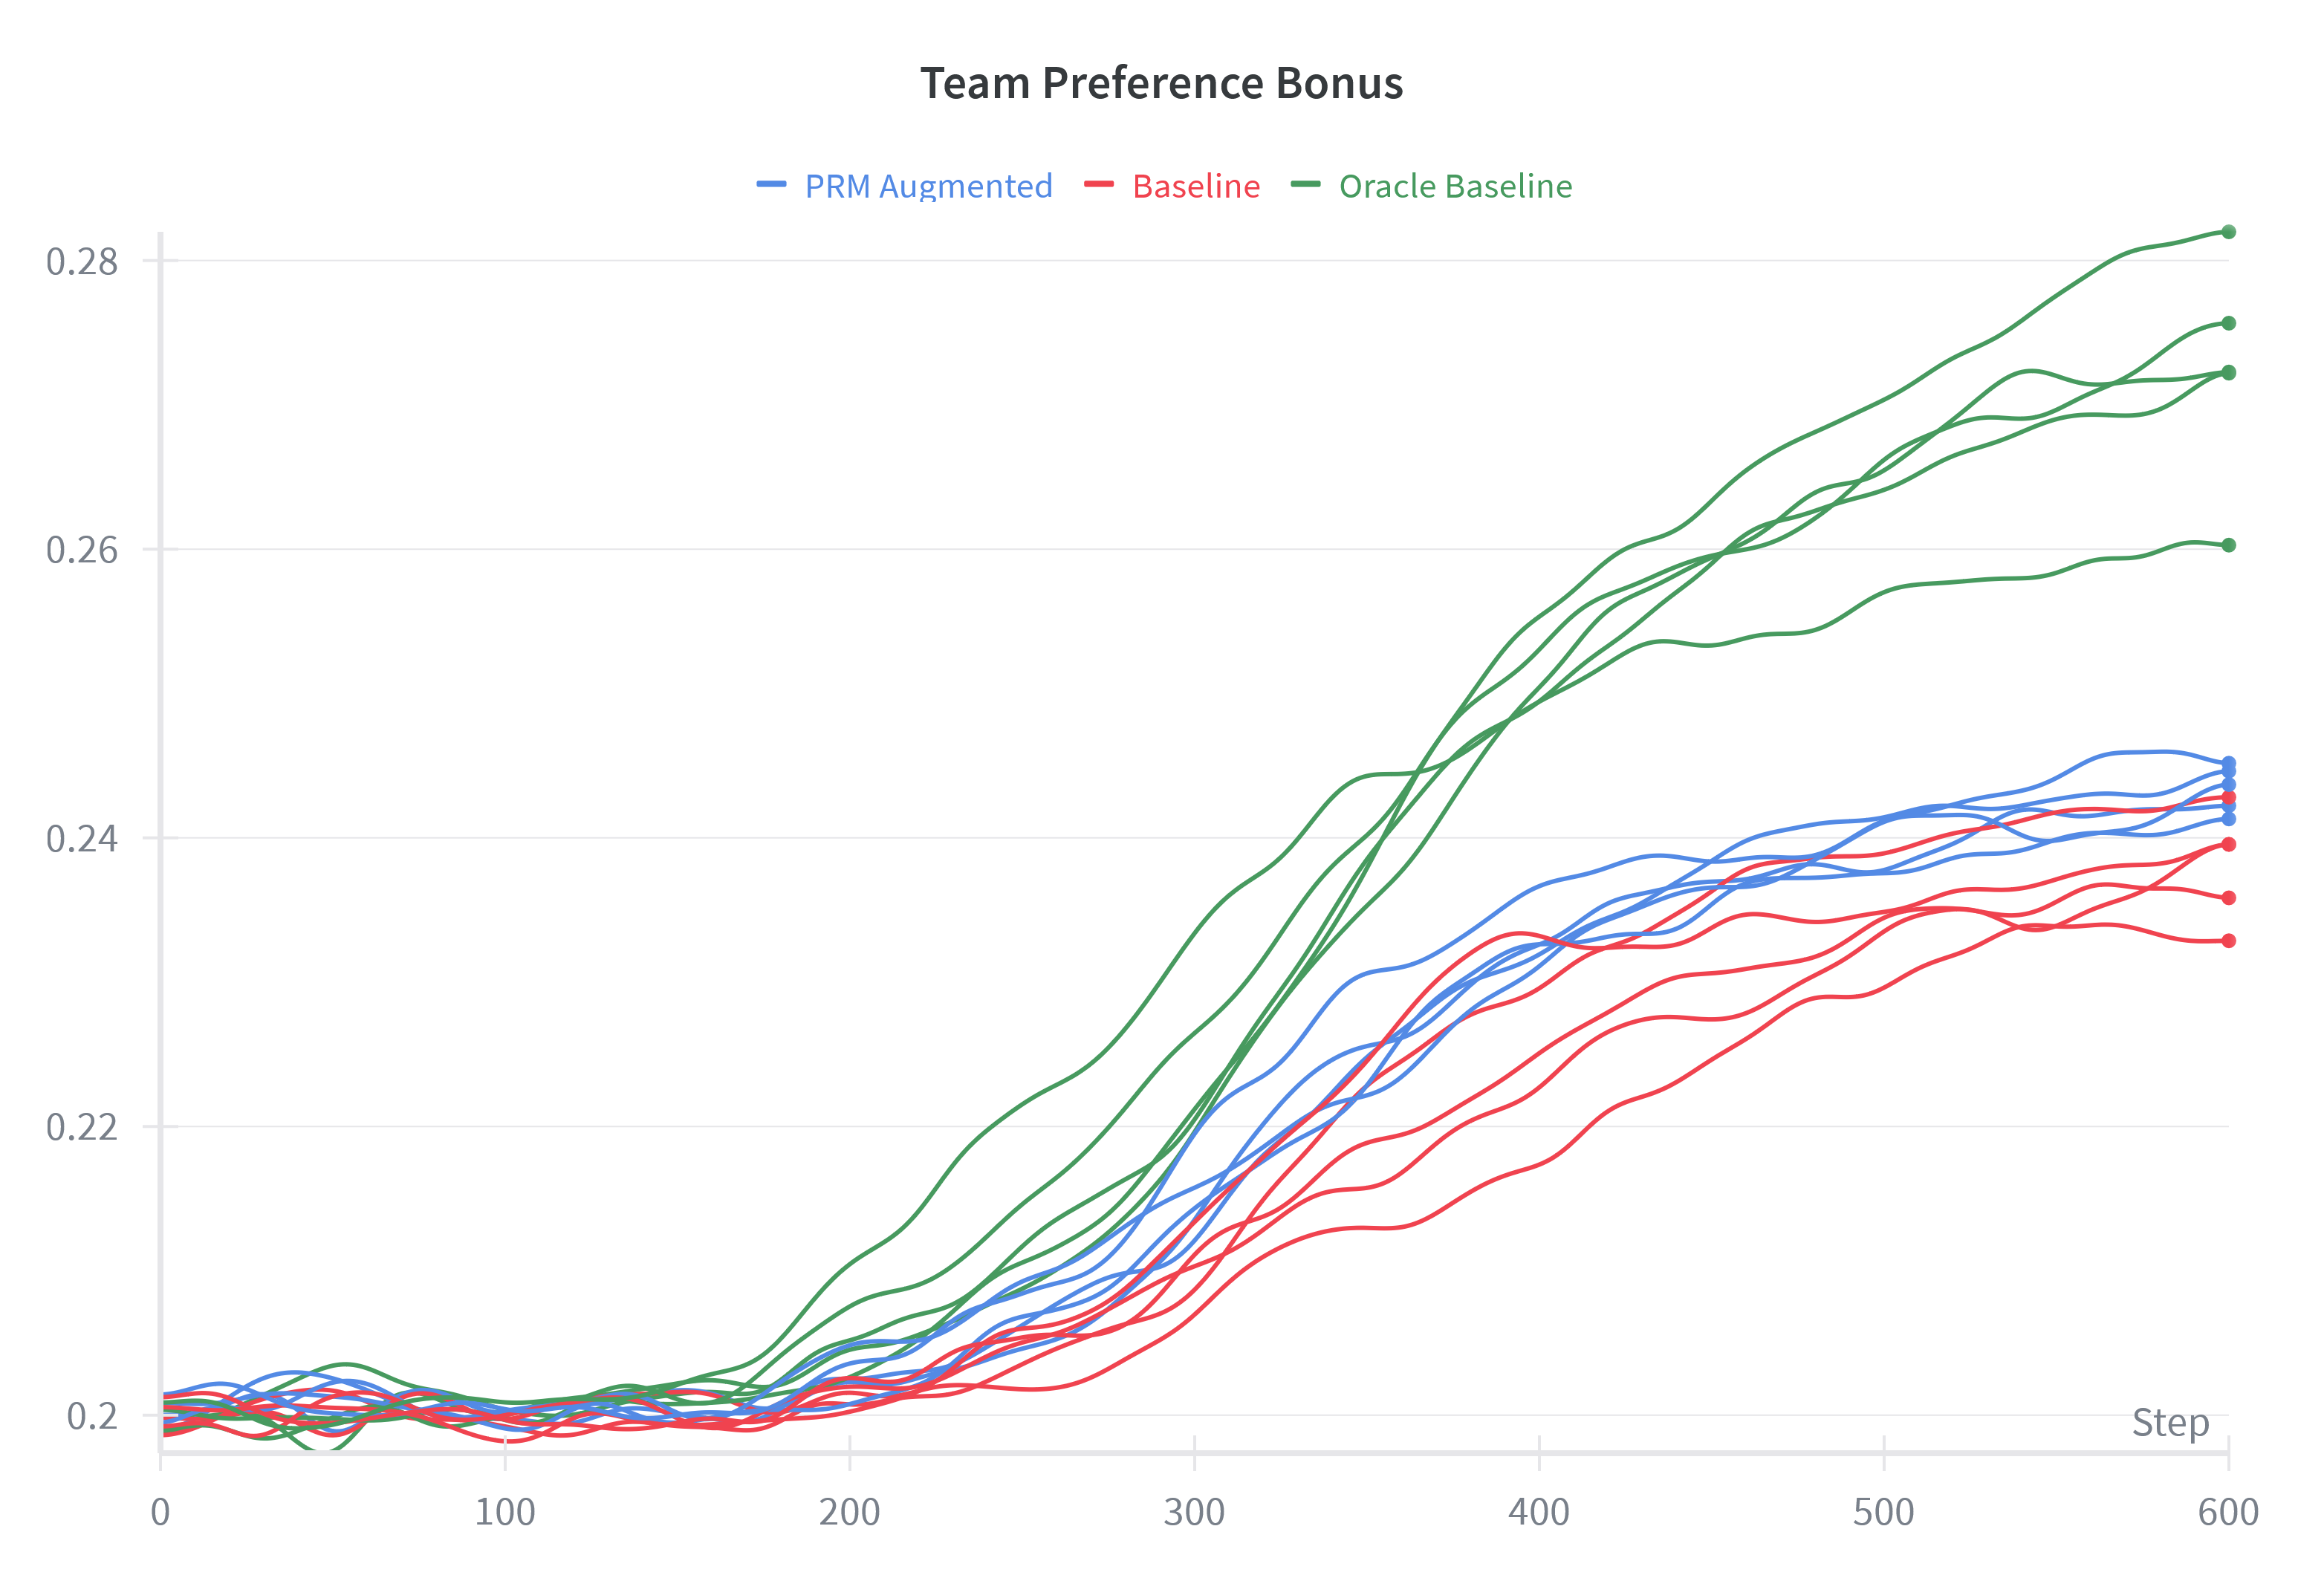
\includegraphics[width=0.7\textwidth]{img/team_pref.png}
    \caption{Mean Preference Bonus. The PRM agent achieves only a marginal gain over the Baseline, far below the Oracle.}
    \label{fig:results_pref_bonus}
\end{figure}

\begin{figure}[h!]
    \centering
    \begin{minipage}{0.49\textwidth}
        \centering
        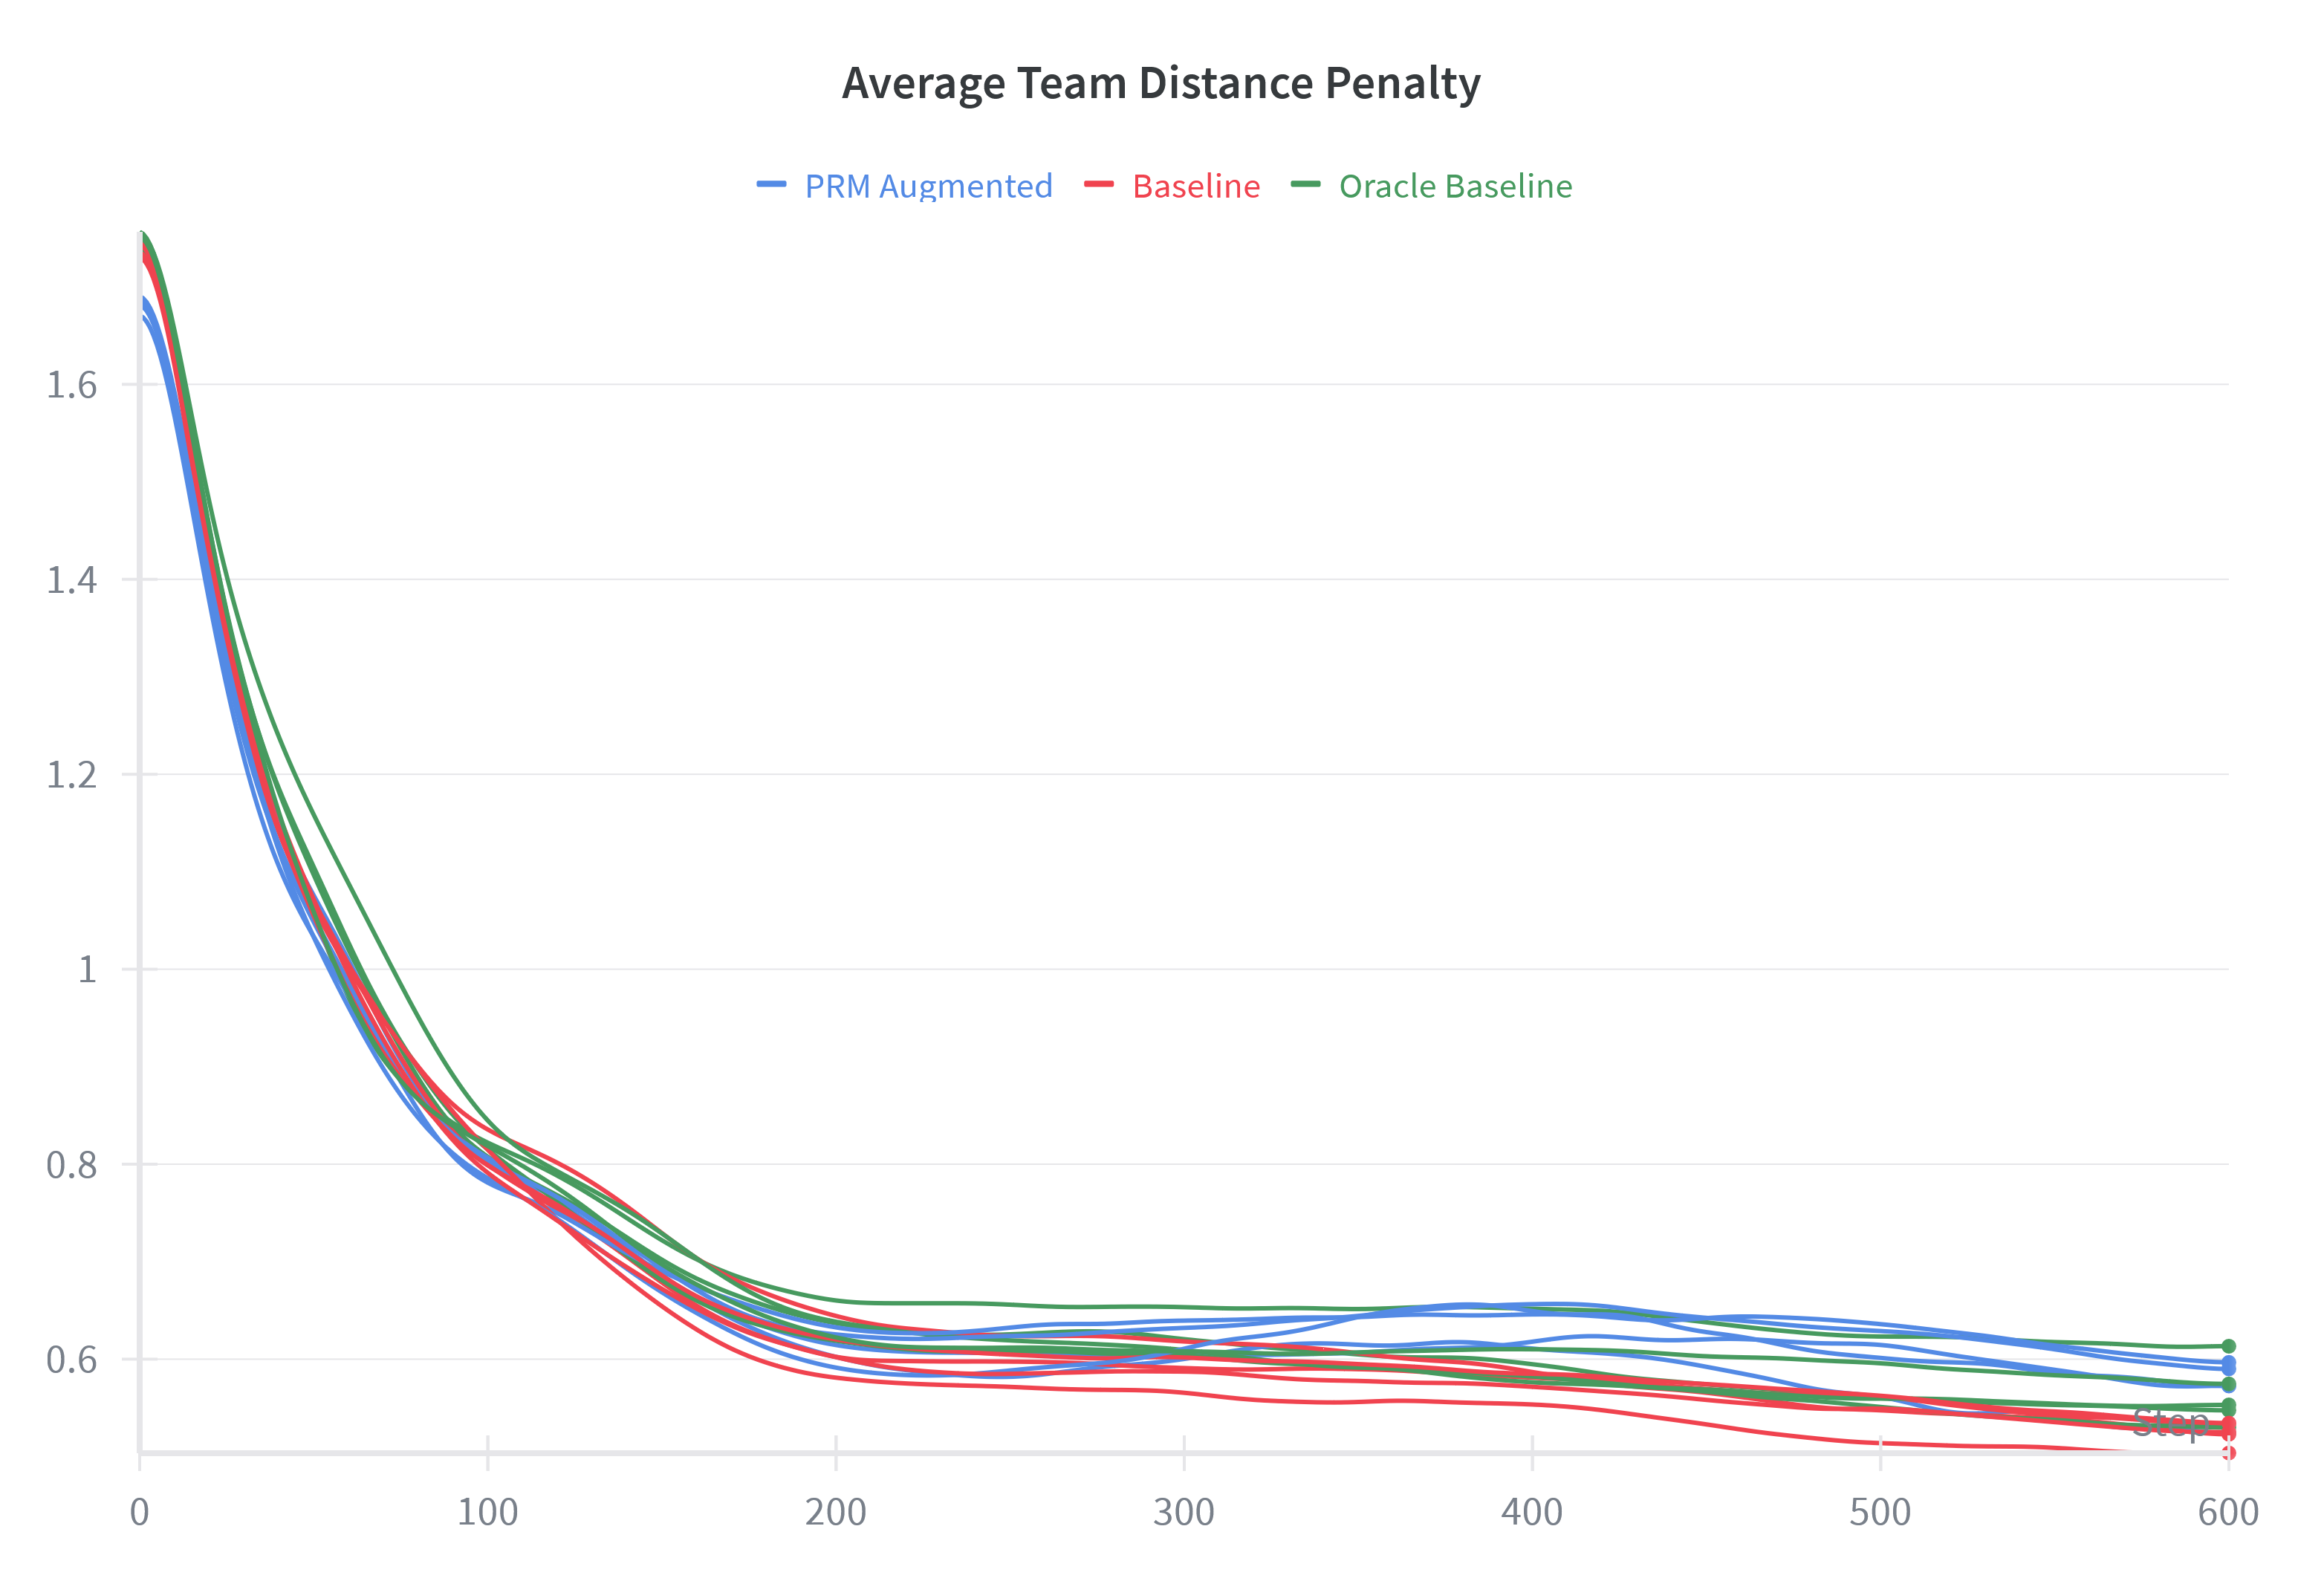
\includegraphics[width=\linewidth]{img/team_dist_pen.png}
        \caption{Mean Team Distance Penalty.}
        \label{fig:results_distance_penalty}
    \end{minipage}\hfill
    \begin{minipage}{0.49\textwidth}
        \centering
        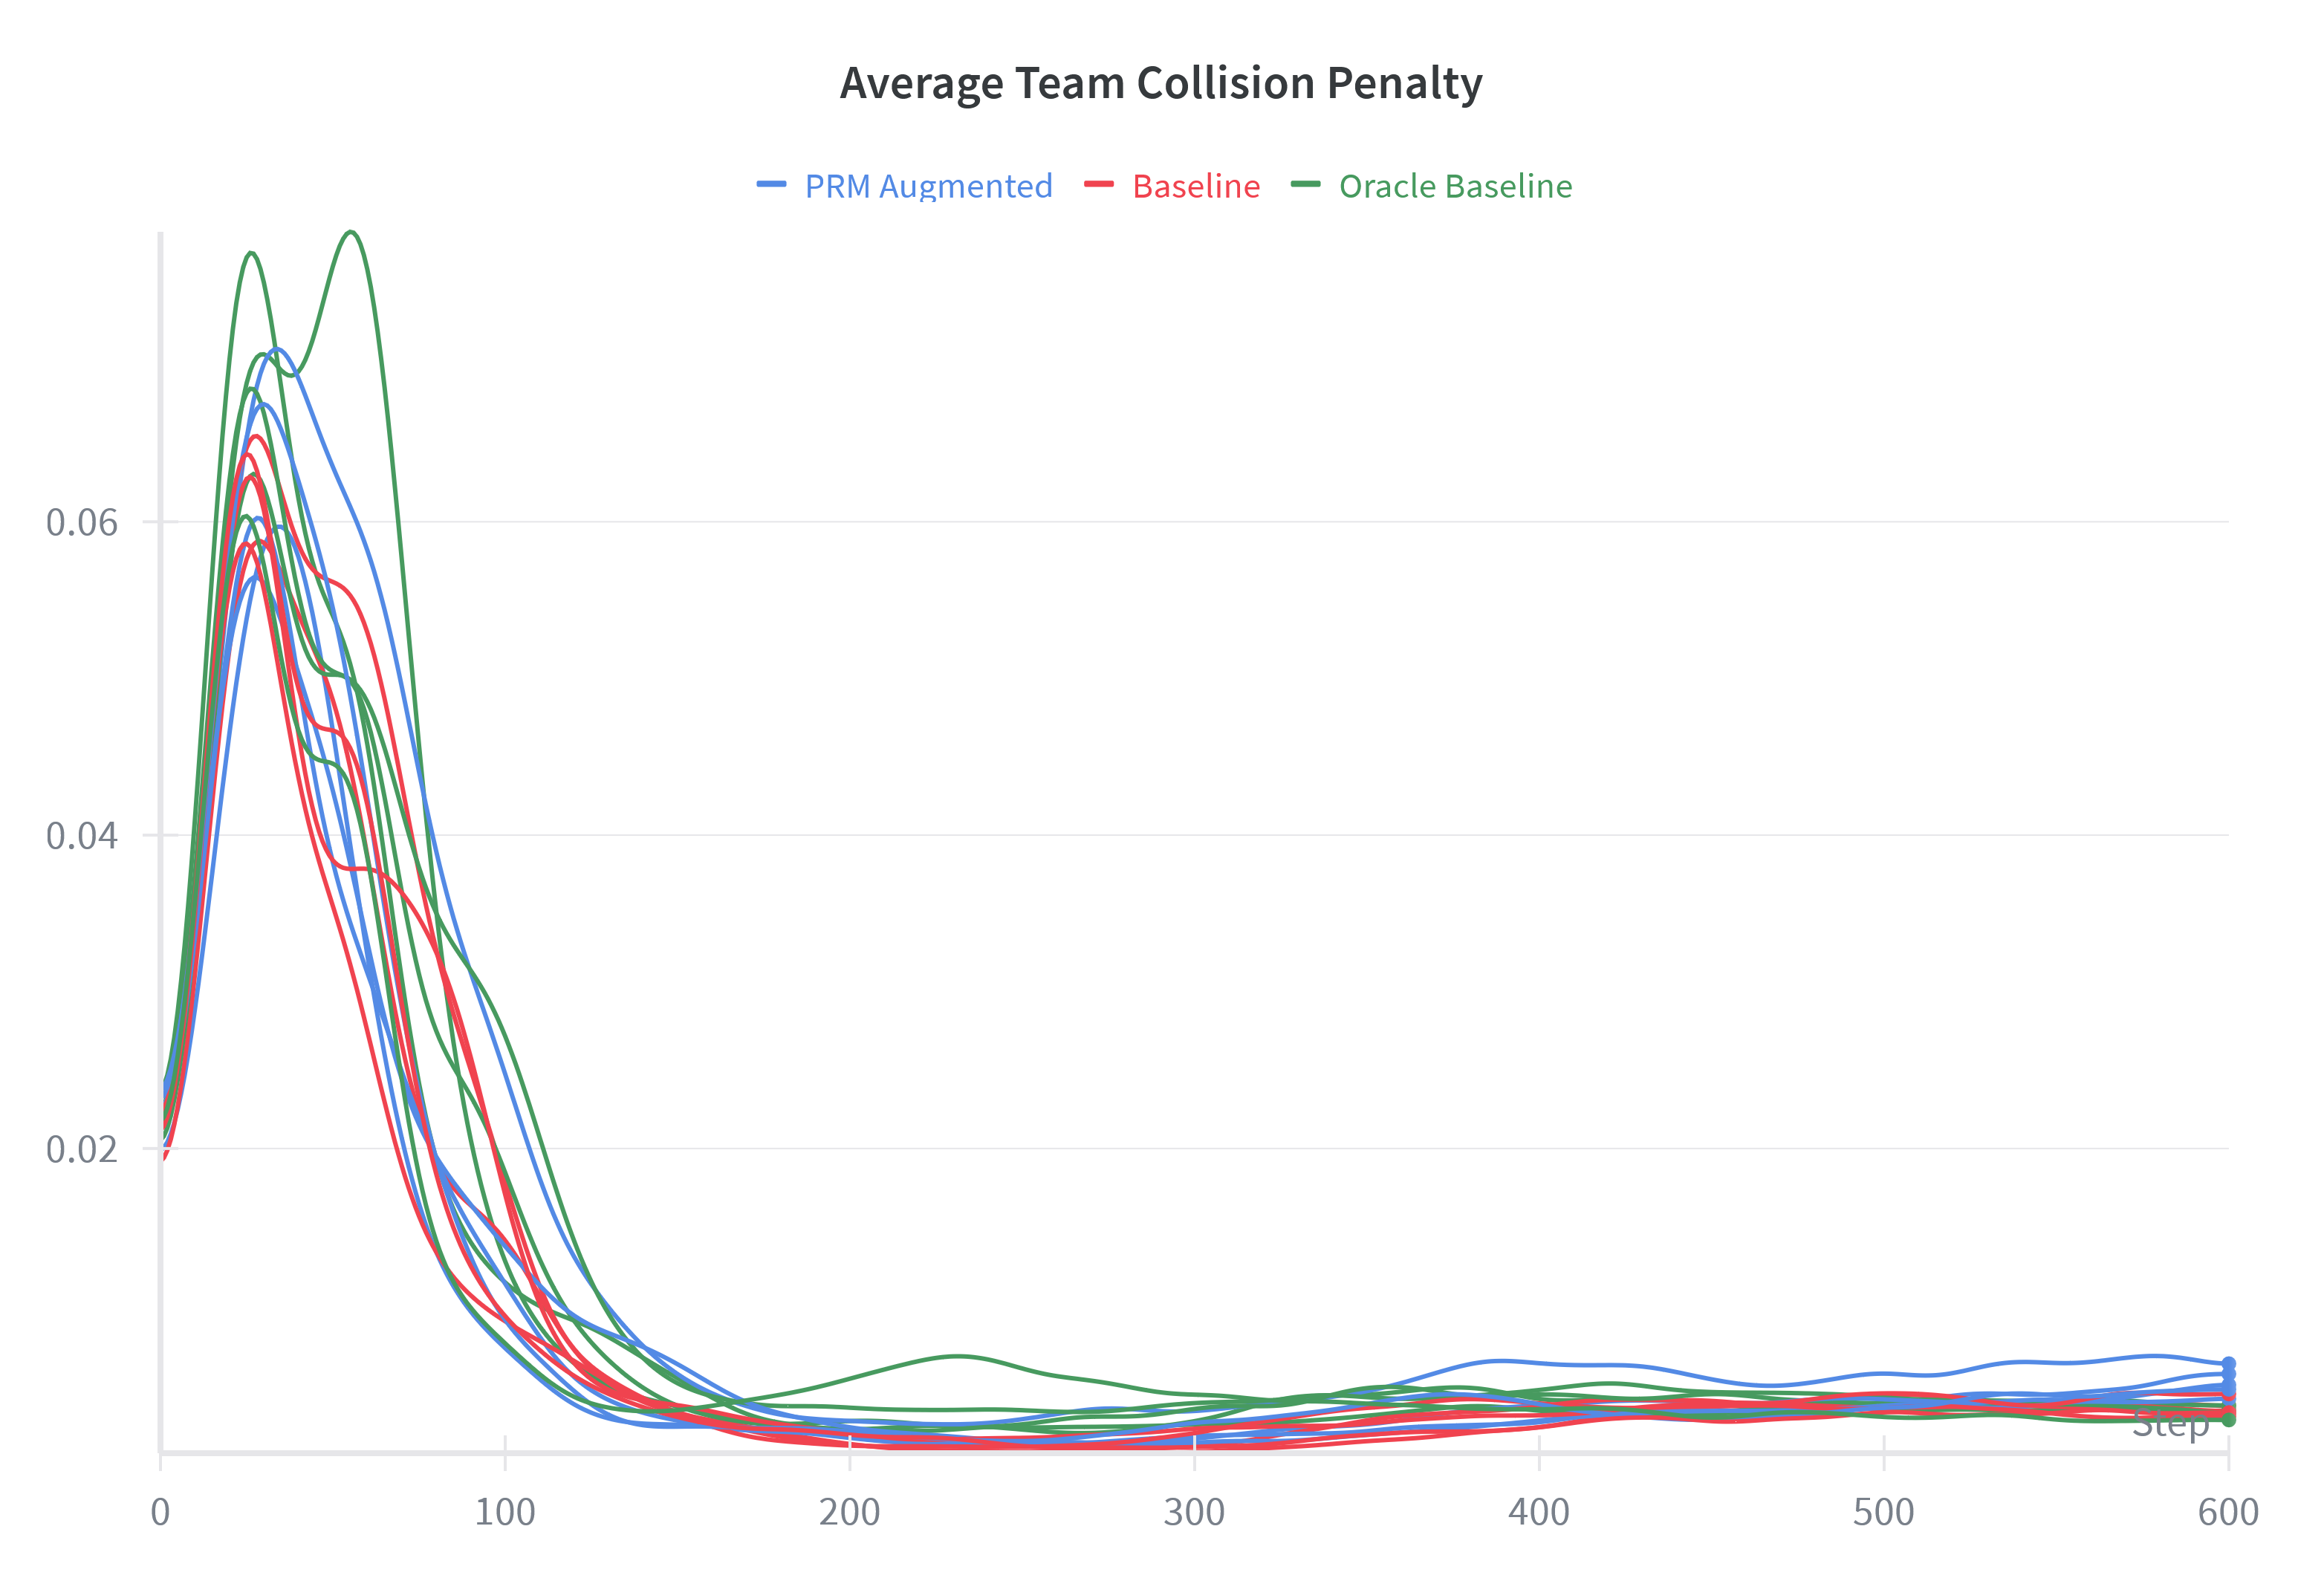
\includegraphics[width=\linewidth]{img/team_coll_pen.png}
        \caption{Mean Team Collision Penalty.}
        \label{fig:results_collision_penalty}
    \end{minipage}
    \caption{Mean Team Penalties (Referenced by \ref{fig:results_distance_penalty} and \ref{fig:results_collision_penalty}). The PRM agent's strategy incurs slightly higher distance and collision penalties than the simpler Baseline policy.}
    \label{fig:results_penalties}
\end{figure}

\section{Analysis of Team-Wide Coherence}
\label{sec:results_coherence}

Finally, we analyze the Team Belief Divergence, which measures the average Jensen-Shannon Divergence (JSD) between the listener beliefs induced by all pairs of agents. This metric provides a final, interesting insight into the PRM agent's behavior, shown in Figure \ref{fig:results_divergence}.

The Standard Baseline agents exhibit the lowest divergence. This suggests the baseline agents are "coherently ambiguous"; they all fail to coordinate in a similar manner, leading to low divergence between their induced beliefs. Conversely, both the PRM-MASAC and Oracle agents exhibit a higher level of belief divergence. This is logical: in order to successfully specialize (which the Oracle does, and the PRM attempts), agents must pursue different goals. These different intentions naturally produce more distinct actions and, consequently, more divergent belief states.

This finding encapsulates the central narrative of these results: the PRM agent \textit{is} behaving like the Oracle in its \textit{intent} to differentiate (higher belief divergence) and its \textit{willingness} to deviate from literal paths (low goal-directedness). However, it fails to execute this strategy in a legible way, which ultimately prevents it from achieving the Oracle's successful division of labor (low specialization).

\begin{figure}[h!]
    \centering
    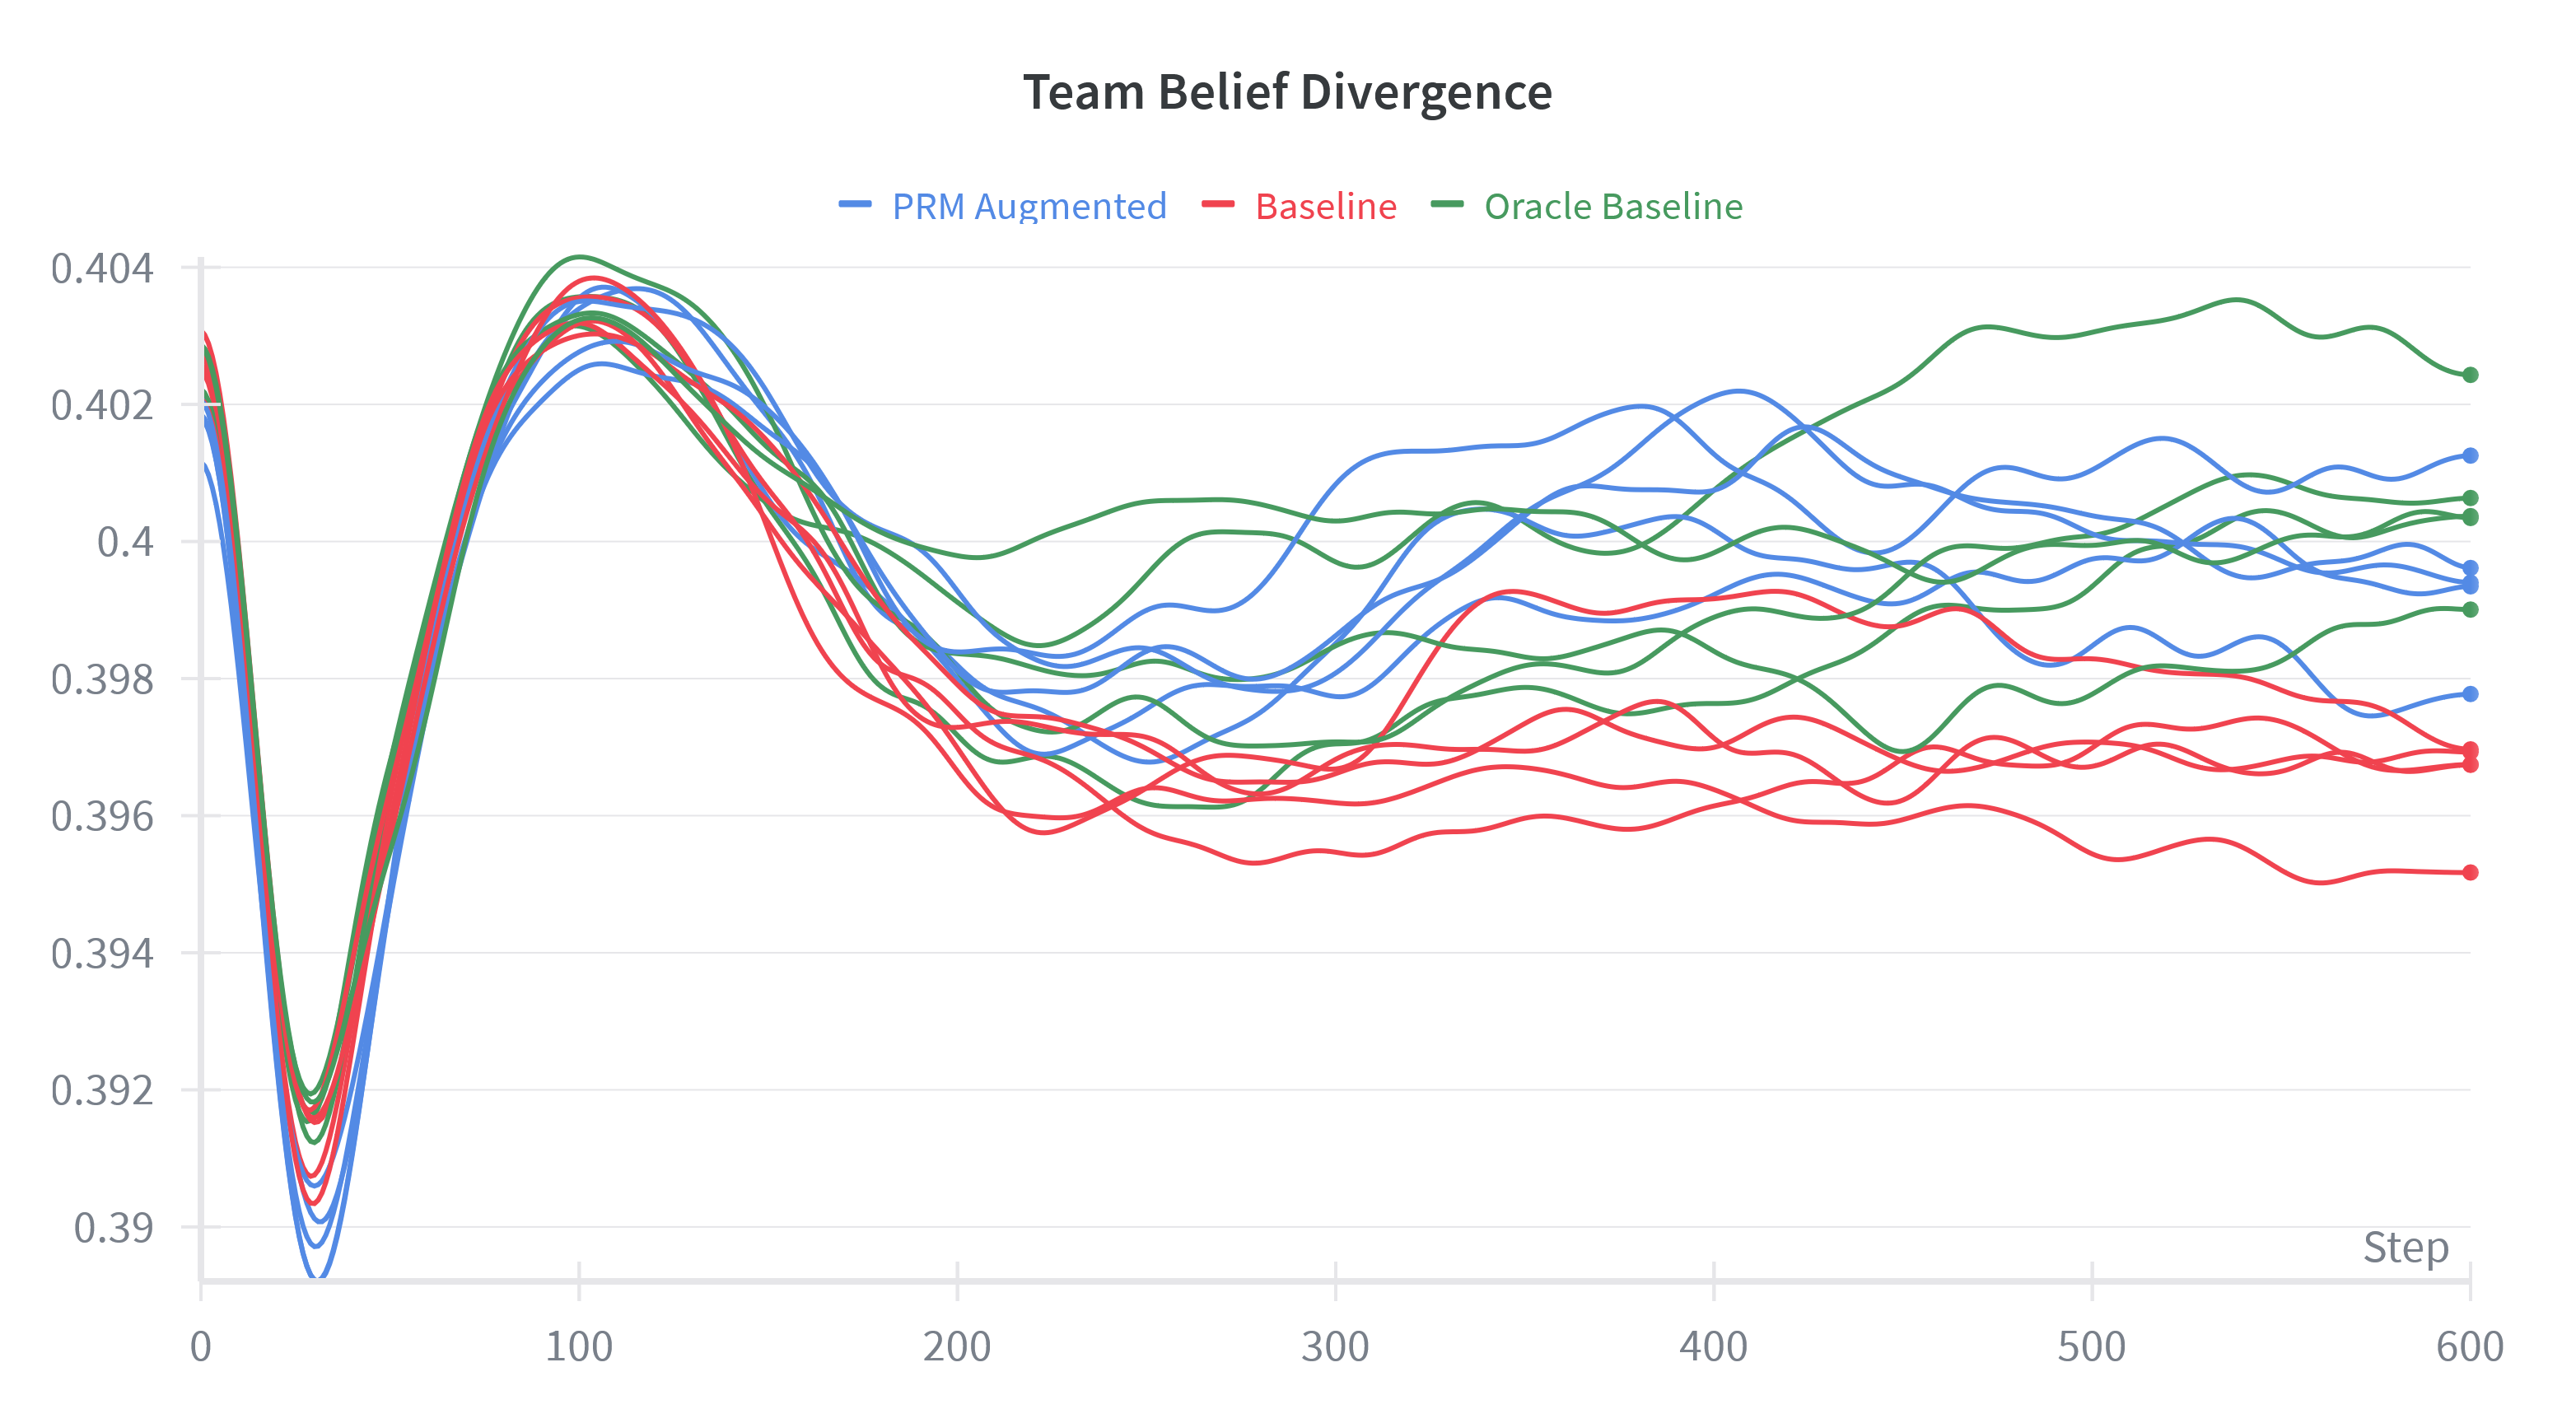
\includegraphics[width=0.9\textwidth]{img/team_belief_divergence.png}
    \caption{Mean Team Belief Divergence (JSD). The PRM agent, like the Oracle, exhibits higher divergence than the Baseline, suggesting an \textit{attempt} to produce differentiated signals, even if those signals are ultimately ineffective.}
    \label{fig:results_divergence}
\end{figure}

\section{Ablation Study: Simplifying the $L_0$ Listener}
\label{sec:results_simple_l0}

The primary analysis in Section \ref{sec:results_communication} and the discussion in Chapter \ref{chap:discussion} identify the complex, heuristic-based $L_0$ listener as a potential source of failure. A key component of this heuristic was the "exclusivity score," designed to explicitly model ambiguity (Algorithm \ref{alg:prm}). We hypothesized that this complex, non-linear scoring might be creating a noisy or unlearnable reward signal.

To test this, we conducted an ablation study using a "Simple $L_0$" model. In this model, we remove the exclusivity score entirely. The literal listener's score for a meaning $m$ given action $a$ is based only on the direct cosine similarity to the ideal path $v_m$:
$$ S_{\text{simple}}(a, m) = \alpha_{\text{temp}} \cdot \cos(a, v_m) $$
The $L_0$ belief is then the softmax over these simple scores. This simplification removes the complex inter-meaning comparison from the base of the pragmatic recursion.

The results, shown in Figure \ref{fig:simple_l0_learnability}, confirm our hypothesis. By simplifying the $L_0$ model, the intrinsic $\Rcomm$ signal becomes significantly more learnable. Unlike the primary experiment (Figure \ref{fig:results_comm_reward}), the agent in this ablation study successfully optimizes the communicative reward, achieving a high, stable $\Rcomm$ value.

However, this learnability did not translate into any other performance benefit. The agent's task-level reward, specialization, and preference bonus were all virtually identical to the standard baseline. This result is crucial: it demonstrates that while the exclusivity score made the $\Rcomm$ signal unlearnable, the simplified signal, even when optimized, was not sufficient to solve the coordination problem. This reinforces the conclusion that the core challenge lies in defining a "common ground" $L_0$ that is both (a) learnable and (b) a valid proxy for true, task-relevant coordination.

\begin{figure}[h!]
    \centering
    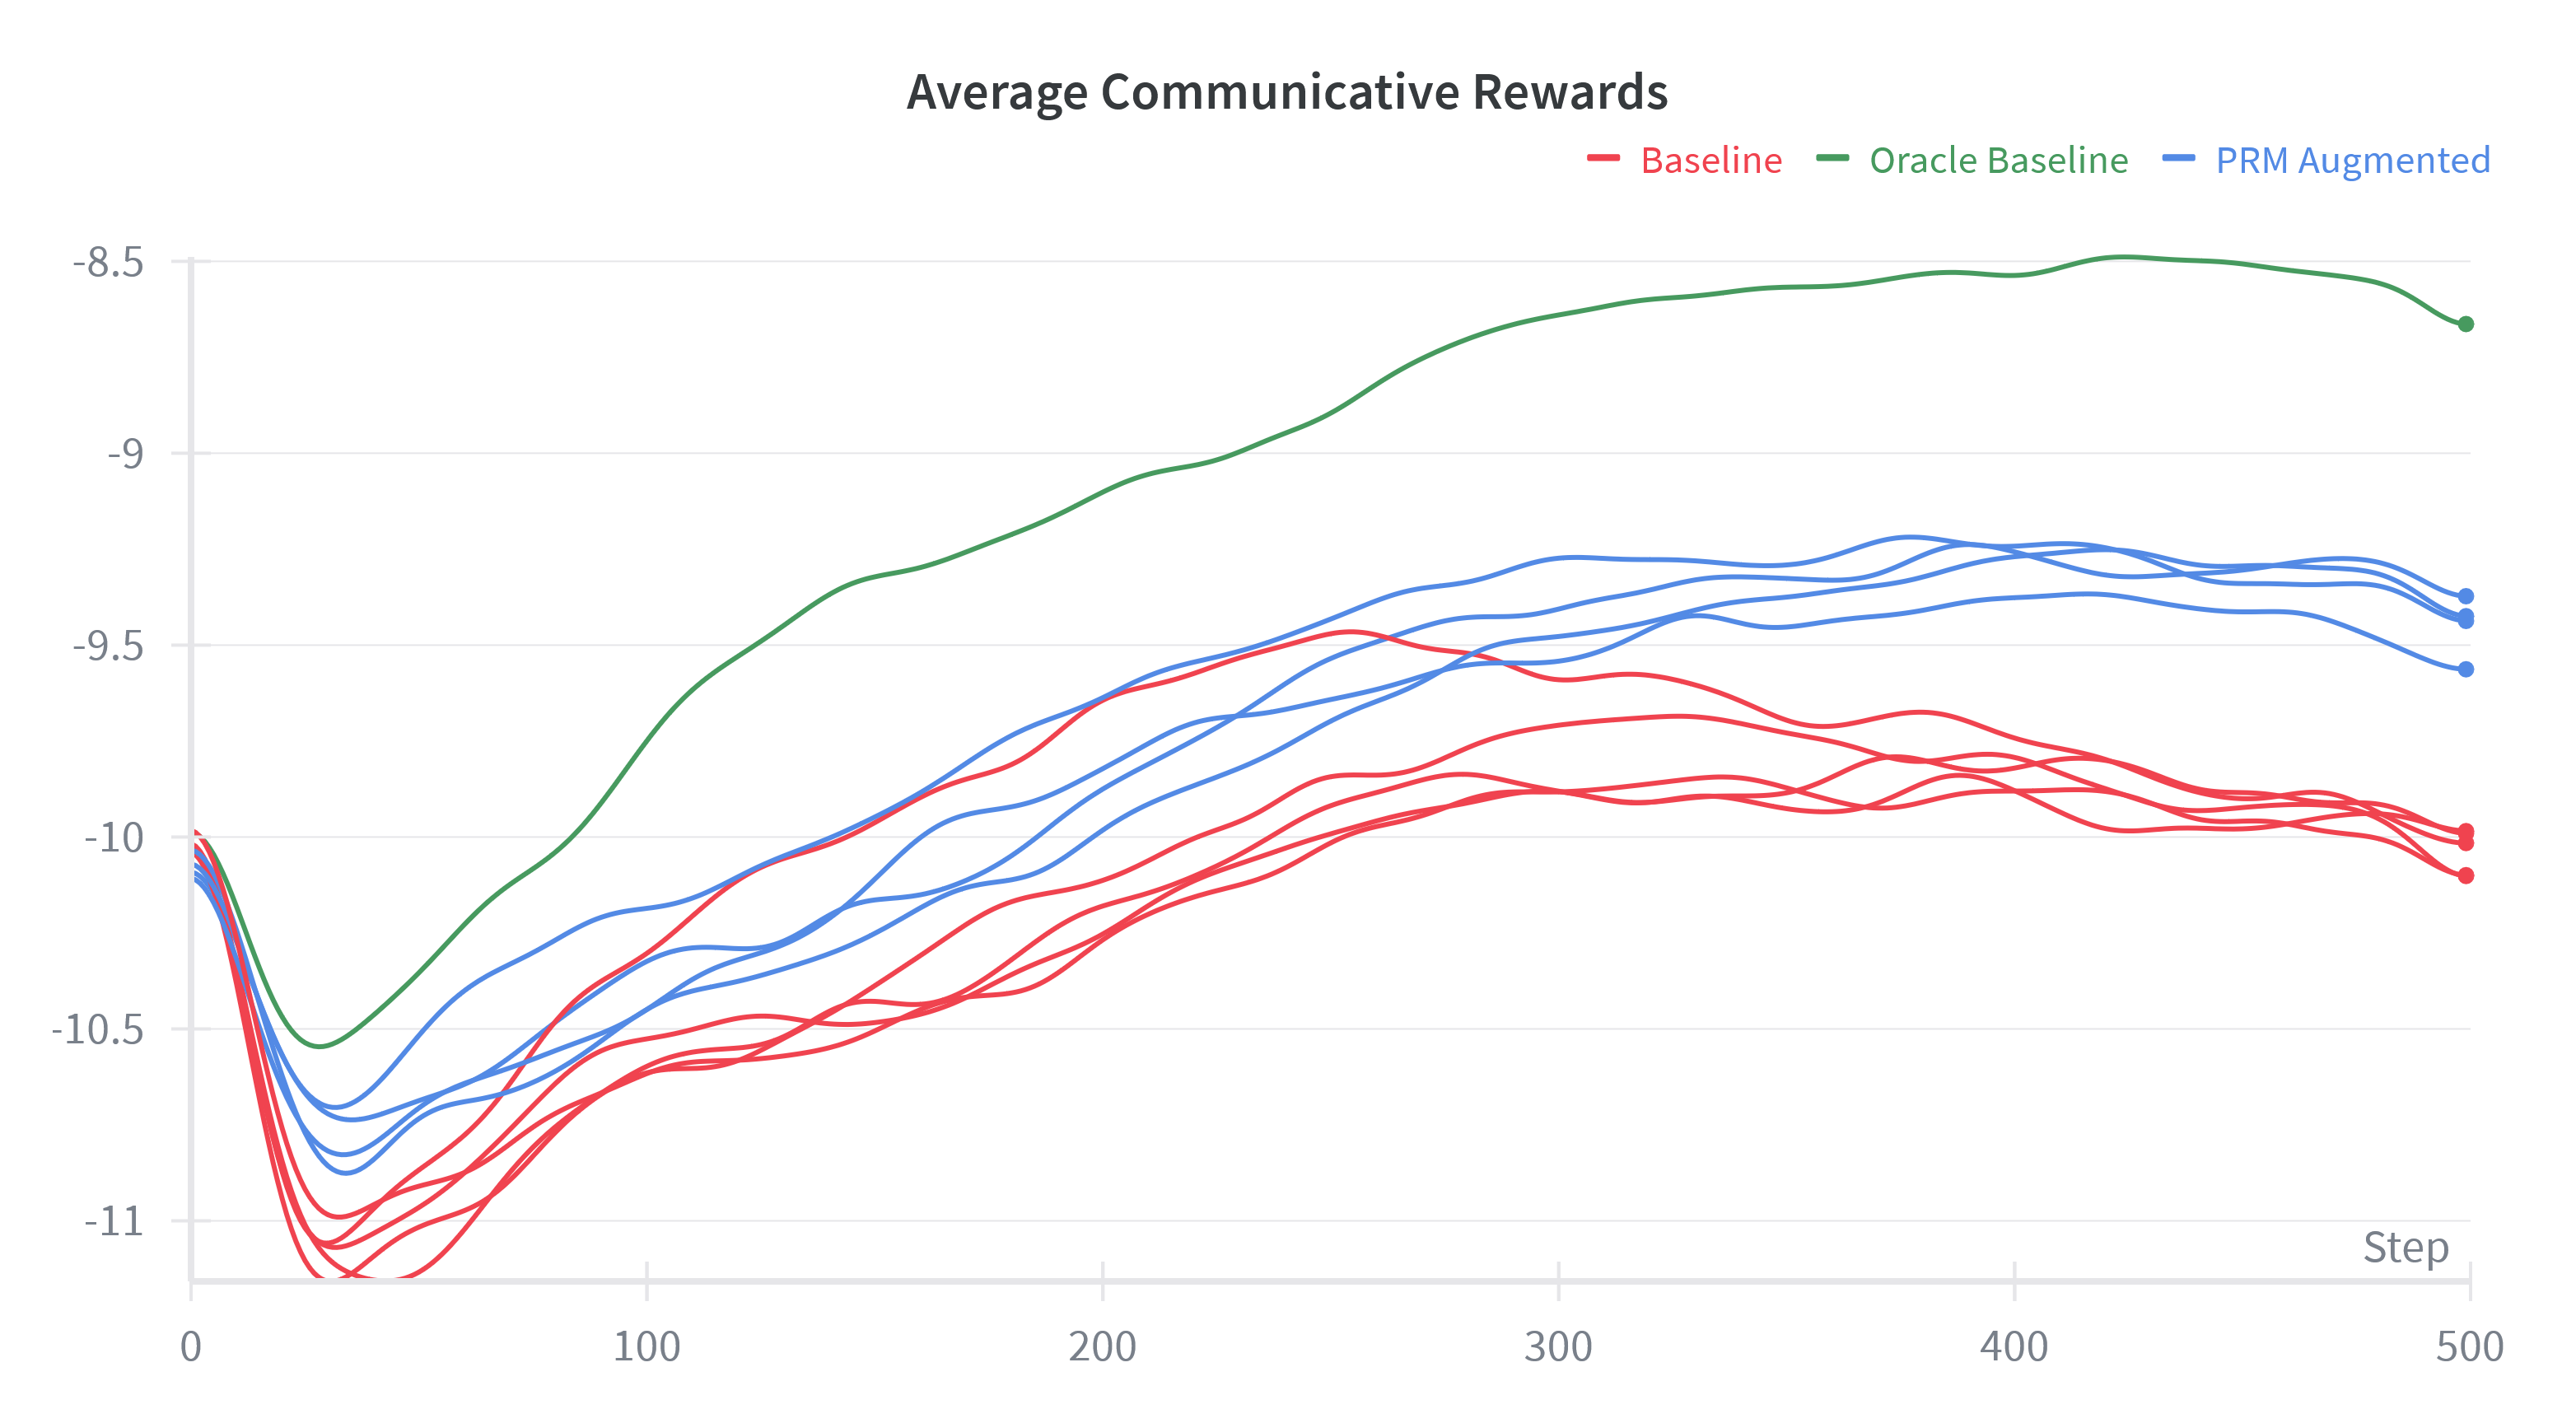
\includegraphics[width=0.8\textwidth]{img/simple_l0.png}
    \caption{Mean Communicative Reward ($\Rcomm$) for the ablation study using the "Simple $L_0$" model. Unlike the main experiment (Figure \ref{fig:results_comm_reward}), the agent successfully learns to optimize this simplified intrinsic reward signal.}
    \label{fig:simple_l0_learnability}
\end{figure}

\section{Qualitative Results}

Qualitative analysis of individual episodes reveals rare instances where the PRM-augmented policy achieves the intended legible coordination, as illustrated in Figure \ref{fig:simple_spread_prm_success}. In these cases, agents successfully signal their distinct intentions, leading to an optimal division of labor and full coverage of all target landmarks.

However, these successful episodes represent statistical outliers. In the vast majority of observed scenarios, the PRM-augmented agent's policy is qualitatively indistinguishable from the standard baseline, typically collapsing into the same uncoordinated and inefficient strategies (as exemplified in Figure \ref{fig:simple_spread_baseline_fail}). Consequently, the minor, infrequent qualitative successes do not outweigh the significant, consistent performance deficits identified in the quantitative analysis (Section \ref{sec:results_performance}), particularly the increased distance and collision penalties. This suggests that while the target behavior is achievable in principle, the current PRM framework fails to provide a sufficiently robust or learnable signal to make this legible strategy the convergent or dominant policy.

\begin{figure}[h!]
    \centering
    
    % --- We use minipages to place images and their labels side-by-side ---
    
    \begin{minipage}{0.32\textwidth}
        \centering
        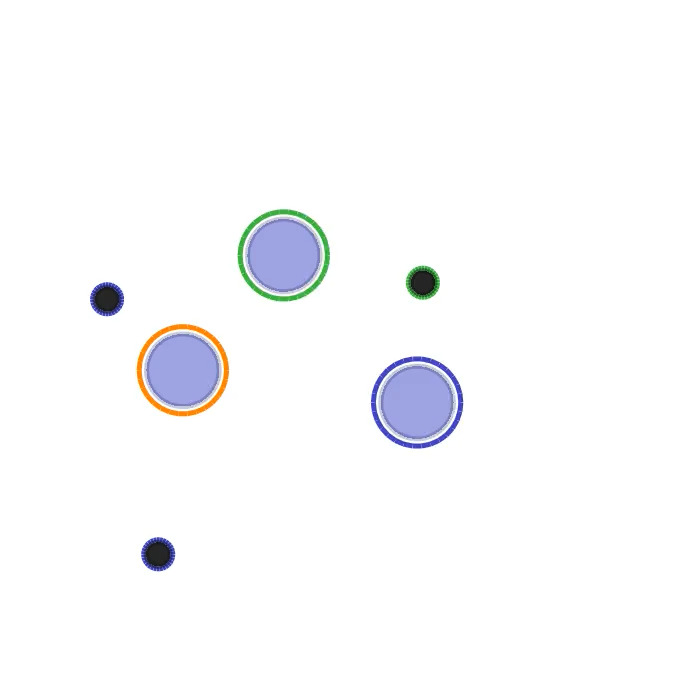
\includegraphics[width=\linewidth, keepaspectratio]{img/initial_frame.jpg}
        \centerline{Episode Start}
    \end{minipage}
    \hfill % Adds horizontal space
    \begin{minipage}{0.32\textwidth}
        \centering
        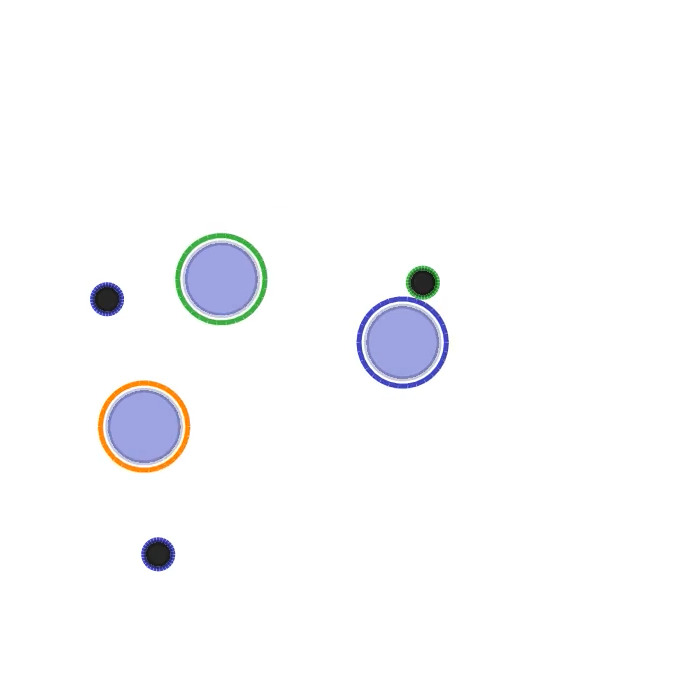
\includegraphics[width=\linewidth, keepaspectratio]{img/base_f2.jpg}
        \centerline{Episode Middle}
    \end{minipage}
    \hfill % Adds horizontal space
    \begin{minipage}{0.32\textwidth}
        \centering
        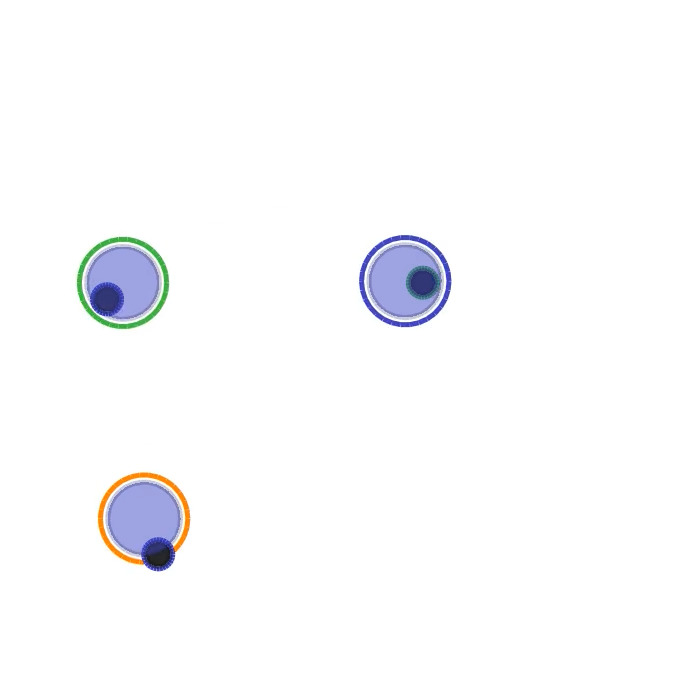
\includegraphics[width=\linewidth, keepaspectratio]{img/base_f3.jpg}
        \centerline{Episode End}
    \end{minipage}
    
    \vspace{5pt} % Adds a small vertical space before the main caption

    % --- Caption with integrated TiKZ Legend ---
    % \protect is needed before \tikz inside a caption to prevent errors
    \caption{
        Agents fail to find an optimal spread with the Baseline policy.
    }
    \label{fig:simple_spread_baseline_fail}
\end{figure}

\begin{figure}[h!]
    \centering
    
    % --- We use minipages to place images and their labels side-by-side ---
    
    \begin{minipage}{0.32\textwidth}
        \centering
        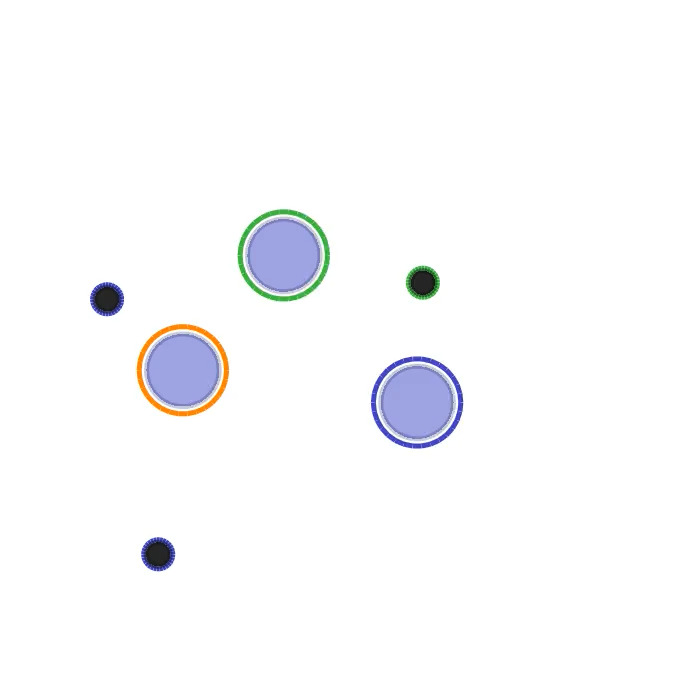
\includegraphics[width=\linewidth, keepaspectratio]{img/initial_frame.jpg}
        \centerline{Episode Start}
    \end{minipage}
    \hfill % Adds horizontal space
    \begin{minipage}{0.32\textwidth}
        \centering
        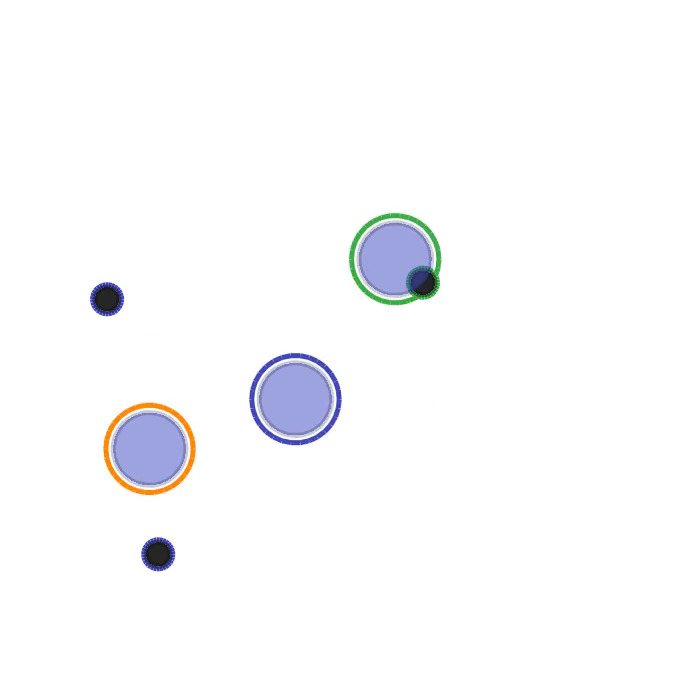
\includegraphics[width=\linewidth, keepaspectratio]{img/prm_f2.jpg}
        \centerline{Episode Middle}
    \end{minipage}
    \hfill % Adds horizontal space
    \begin{minipage}{0.32\textwidth}
        \centering
        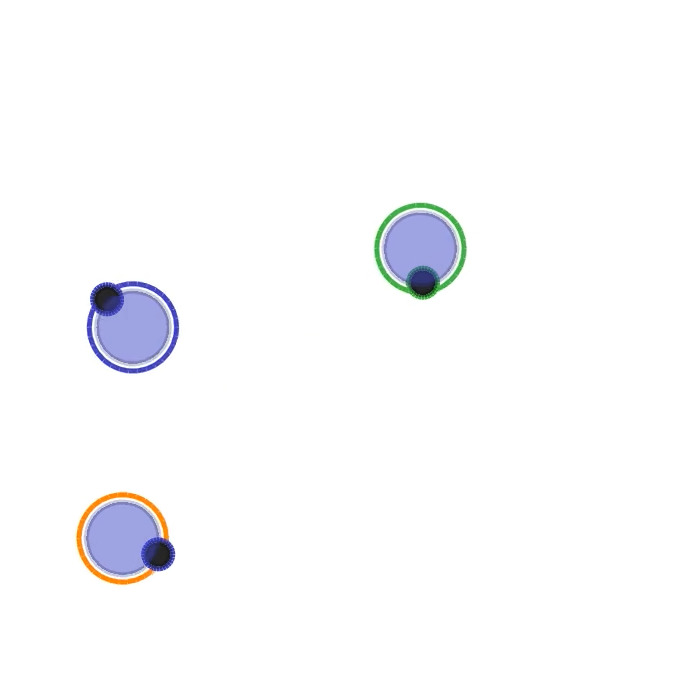
\includegraphics[width=\linewidth, keepaspectratio]{img/prm_f3.jpg}
        \centerline{Episode End}
    \end{minipage}
    
    \vspace{5pt} % Adds a small vertical space before the main caption

    % --- Caption with integrated TiKZ Legend ---
    % \protect is needed before \tikz inside a caption to prevent errors
    \caption{
        Agents correctly signal their meanings and reach an optimal spread under the PRM-Augmented policy.
    }
    \label{fig:simple_spread_prm_success}
\end{figure}

%---------------------------------------------------------------------
%   9. CRITICAL DISCUSSION (5 pages)
%---------------------------------------------------------------------
\chapter{Critical Discussion}
\label{chap:discussion}

The empirical results presented in Chapter \ref{chap:experiments_results} provide a complex and informative picture of the proposed framework. The findings reveal a significant contradiction: while the Pragmatic Reward Module (PRM) successfully induced a distinct \textit{behavioral} policy, this policy failed to achieve the \textit{communicative} or \textit{task-level} objectives it was designed to solve. This chapter analyzes this central contradiction, identifies the hypothesized sources of this failure, and discusses the broader limitations of the study.

\section{Analysis of the Experimental Contradiction}
The primary finding from our experiments is the clear divergence between behavioral change and communicative success. The PRM-MASAC agent learned a policy characterized by significantly lower goal-directedness (Figure \ref{fig:results_goaldirectedness}) and higher action magnitude (Figure \ref{fig:results_magnitude}) compared to the Standard Baseline. This demonstrates that the composite reward $\Rtotal = \Rext + \lambda \Rcomm$ was operative; the intrinsic $\Rcomm$ signal was strong enough to compel the agent to learn a "costly" policy, sacrificing the shortest-path-to-goal efficiency that a pure $\Rext$ optimizer would prefer. This confirms that the framework can, in principle, incentivize agents to deviate from "literal" behavior.

However, this costly signaling strategy proved entirely ineffective. The agent's performance on the primary communicative metrics---Communicative Clarity (Figure \ref{fig:results_comm_clarity}) and the Communicative Reward itself (Figure \ref{fig:results_comm_reward})---was indistinguishable from the baseline. Furthermore, this communicatively-ineffective signaling failed to solve the core coordination problem, as evidenced by the lack of improvement in Team Specialization (Figure \ref{fig:results_specialization}). The marginal gains in preference bonus (Figure \ref{fig:results_pref_bonus}) were offset by higher distance and collision penalties (Figure \ref{fig:results_penalties}), resulting in no meaningful improvement in overall task performance.

The most telling result may be the Team Belief Divergence (Figure \ref{fig:results_divergence}). The PRM agent, like the Oracle, exhibited high divergence, in contrast to the "coherently ambiguous" baseline. This suggests the PRM agents \textit{were} attempting to differentiate themselves and pursue distinct goals, just as the Oracle agents did. The failure, therefore, was not in the \textit{intent} to specialize, but in the \textit{execution} of a legible strategy to communicate that intent. The agents learned to "talk," but were speaking "incoherently."

\section{Hypothesized Sources of Failure}
This central contradiction points to several critical flaws in the framework's current instantiation, moving the original "Weaknesses" (as posited in the template) to the forefront as the primary explanation for the negative results.

\subsection{The $L_0$ "Common Ground" Problem}
The most likely source of failure is the "common ground" problem, encapsulated by the heuristic literal listener model, $L_0$. The entire pragmatic reward $\Rcomm$ is calculated relative to this $L_0$, which functions as the assumed, shared basis for interpreting actions. We engineered a specific "exclusivity score" heuristic (Algorithm \ref{alg:prm}) based on relative cosine similarity, believing it would effectively capture ambiguity.

The results strongly suggest this heuristic was flawed. The agent learned behaviors (low goal-directedness) that were "surprising" or "deviant" relative to this $L_0$, but these deviations did not, in fact, map to "clarity" for the recursive pragmatic listener $L^*$. If the $L_0$ foundation is "wrong"---if it does not accurately model the salient features of ambiguity in the environment---then the entire recursive tower of reasoning built upon it is also wrong. The agent may be optimizing for a reward signal that is, at best, a poor proxy for true legibility and, at worst, an arbitrary and noisy signal that encourages inefficient behavior for no communicative benefit.

\subsection{A Flawed or Unlearnable Reward Signal}
A related possibility is that the final $\Rcomm$ signal, derived from the pragmatic listener $L^*$, is itself unlearnable. The agent's demonstrable failure to optimize its own intrinsic reward (Figure \ref{fig:results_comm_reward}) is a serious indictment. This pragmatic reward, calculated via sampling and recursive softmax operations, may be too sparse, noisy, or complex for the agent's value function to accurately model. The agent may have settled into a poor local optimum, where it learned to execute the most "obvious" form of signaling (deviating from the shortest path) but could not discover the more subtle, precise behaviors that would have successfully maximized the $L^*$ score. This suggests a failure in the credit assignment or optimization landscape, where the agent found it easier to "game" the $L_0$ heuristic than to genuinely solve the $L^*$ pragmatic objective.

\subsection{Destructive Interference and the $\lambda$ Trade-off}
Finally, the results indicate a clear case of destructive interference between the two reward components. The agent's costly signaling strategy directly resulted in higher distance and collision penalties (Figures \ref{fig:results_penalties}). This demonstrates that the pursuit of $\Rcomm$ actively harmed the agent's ability to optimize $\Rext$. This is the "performance art" failure case hypothesized during the framework's design: the agent over-optimized for a flawed communicative signal at the direct expense of task completion. The chosen $\lambda$ value, while intended to provide a gentle "nudge" toward legibility, instead appears to have created a conflicting objective that the agent could not successfully balance, leading to a policy worse than the baseline that simply focused on the task at hand. This hypothesis is supported by our ablation study (see Appendix \ref{chap:ablations}, Figure \ref{fig:lambda_tpf}), which demonstrates that even a modest $\lambda$ value of $0.05$ severely degrades task performance, while smaller values are simply ignored by the agent as noise.

\subsection{Insufficiency of Evaluation Metrics}
A further possibility is that the failure is not in the agent's strategy but in our capacity to measure it. The evaluation metrics employed, while standard, are fundamentally aggregative and may lack the granularity to represent the behavioral subtleties of an emergent communicative protocol. Metrics such as Communicative Clarity or Team Specialization are computed on a per-step or per-episode basis, potentially obscuring more complex, temporally-extended strategies. For instance, an action that appears "ambiguous" in isolation---and is thus penalized by the myopic $\Rcomm$ calculation---could be a crucial component of a multi-step "signaling phrase" that only becomes legible to a partner when observed as part of a longer sequence. The current metrics, which are not designed to capture such sophisticated, path-dependent forms of coordination, might therefore incorrectly register a complex, emergent strategy as a simple failure.

\section{Limitations of the Study}
The claims resulting from this research must be interpreted within the specific boundaries of the experimental design, which remain limitations regardless of the results.

The most significant limitation is the exclusive use of AI-AI interactions. The thesis is motivated by human-agent teaming, but we provide no empirical evidence that "computational legibility" translates to "human-perceived legibility." Indeed, this study's failure highlights that even a computationally-defined listener may not be a valid model, strengthening the need to validate any legibility model against actual human partners.

A second, and perhaps more fundamental, limitation lies in the definition and operationalization of "meaning" ($m_t$). In this study, $m_t$ was defined as a hand-crafted, problem-dependent, discrete variable. This approach may lack generalizability to more complex domains where an agent's "intention" is not a simple category but rather a continuous variable (e.g., a precise target location) or a complex, hierarchical plan. The current framework does not offer a clear methodology for computing $\Rcomm$ over such high-dimensional or abstract "meaning spaces."

A further limitation stems from the prohibitive computational cost associated with training these complex multi-agent models, as well as the size of the hyperparameter space. This expense constrained the total number of independent training seeds, effectively limiting the sample size for our experiments. Consequently, a rigorous statistical analysis, such as the generation of robust confidence intervals, was not feasible within the scope of this project. This prevents a statistically significant quantification of the performance differences between our framework and the baselines, confining our analysis primarily to the observed mean trends.

Lastly, the scope of our empirical validation was confined to relatively simple, 2D particle environments and assumed homogeneous teams. The robustness and adaptability of this framework (even if it were successful) in more complex, high-dimensional state spaces, or within heterogeneous teams, remain open questions.

\section{Reflective Feedback on the Work}
This project was an ambitious attempt to bridge the formalisms of computational pragmatics and deep reinforcement learning. While it is disappointing to achieve mixed results, this outcome is also exciting, as it reveals numerous avenues for extending and exploring these ideas---many of which are ``low-hanging fruit'' for subsequent work. The inability to test every hypothesis due to the internship's time constraints is frustrating, but the work of refinement continues.

The central hypothesis was that the RSA framework, imported as an intrinsic reward, could provide a principled signal for emergent coordination. The clear negative results were initially surprising but are, in retrospect, highly informative. They highlight a critical and often-understated challenge in research on "legible AI": the design of the "observer" model (our $L_0$) is not a simple engineering choice but is, in fact, the core of the problem. As this research has made clear, the ``little choices,'' such as the precise formulation of the $L_0$ common ground, can make all the difference.

Our framework's failure demonstrates that a hard-coded, heuristic-based model of "common ground" is insufficient. The agent's policy and the observer's model must be aligned, and this alignment likely cannot be pre-specified. Although this particular implementation was not successful, this does not mean we should bury this line of inquiry. What was learned is that naively bridging these two fields is not enough. The "listener" itself must be a part of the learning process. The failure of this experiment does not invalidate the theoretical bridge but rather demonstrates that the practical implementation requires a co-adaptive approach, where the "literal listener" $L_0$ is not a static heuristic but a dynamic model, learned alongside the agent's policy. This moves the challenge from reward design to representation learning, learning a shared embedding space for actions and intentions.

%---------------------------------------------------------------------
%   10. CONCLUSION AND PERSPECTIVES (2 pages)
%---------------------------------------------------------------------
\chapter{Conclusion and Perspectives}
\label{chap:conclusion}

\section{Assessment of Objectives}
We now revisit the three primary objectives set forth in the introduction.

The scientific objective--to establish a formal theoretical bridge between Maximum Entropy Reinforcement Learning and the Rational Speech Act framework---was \textbf{met}. The derivation in Chapter 5 successfully unified the two formalisms, mapping RSA's "listener value" ($V_L$) to a Max-Ent RL reward component, $\Rcomm$.

The technical objective--to design and implement a "Pragmatic Reward Module" (PRM) based on this bridge--was also \textbf{met}. We successfully implemented this module (Algorithm \ref{alg:prm}) and integrated it into a centralized training (CTDE) loop with the MASAC algorithm.

However, the applicative objective--to demonstrate empirically that this framework produces agents with improved team performance and enhanced legibility--was not met. The empirical results in Chapter \ref{chap:experiments_results} clearly showed that our PRM-MASAC implementation failed to outperform significantly the baseline. The agents' behaviors changed, but this did not lead to measurably improved legibility or more effective team coordination. Instead, the results highlighted the critical flaws in the framework's practical instantiation, particularly its reliance on a static, heuristic-based "common ground."

\section{Main Contributions}
Despite the negative experimental outcome, this thesis provides several contributions:

\begin{itemize}
    \item A  formal derivation that unifies the decision-making models of Maximum Entropy Reinforcement Learning and the Rational Speech Act framework, providing a theoretically-grounded basis for an intrinsic legibility reward.

    \item A hybrid MARL architecture (the Pragmatic Reward Module) that operationalizes this theory, demonstrating how a complex, non-Markovian reward signal based on pragmatic inference can be computed during centralized training.

    \item A critical empirical analysis of this framework, providing a valuable "negative result" for the community. Our findings demonstrate that this direct unification, when reliant on a hand-crafted literal listener ($L_0$), is insufficient. The resulting agents adopt "costly signaling" strategies that are communicatively ineffective and fail to improve task performance, thereby pinpointing the $L_0$ common ground model as the primary point of failure.
\end{itemize}

\section{Perspectives and Future Work}
The failure of this specific implementation does not invalidate the underlying theory but rather illuminates a more promising path forward. Future work should abandon static, heuristic-based listeners and instead focus on \textit{learning} the common ground.

\subsubsection{Learning the Listener Model}
The most critical next step is to replace the hard-coded $L_0$ model. A more robust approach would be to train an auxiliary "listener network" as part of the architecture. This network would be trained (e.g., via supervised learning on the replay buffer) to predict an agent's true private state $m_t$ from its observed action $a_t$ and the public state $s_t$. The pragmatic reward $\Rcomm$ could then be derived from this learned listener. This would co-adapt the agent's policy ("speaker") and the "listener" model, forcing them to align on a useful, emergent communication protocol.

\subsubsection{Dynamic and Self-Assigned Meanings}
A significant limitation of the current framework is its reliance on a hand-crafted, static, and discrete "meaning space" ($\mathcal{M}$). A challenging but promising avenue for future work is the exploration of dynamic and self-assigned meanings. In this paradigm, an agent would not be \textit{given} a fixed $m_t$ to communicate, but would instead learn \textit{what} information is most critical to signal to its partners at any given time. This meaning could be a higher-level abstract concept, such as an overall "strategy" it intends to execute (e.g., "I will distract," "I will cover the flank"), a dynamically updated preference based on the current state, or a compressed representation of its local observations or belief state. This would require the agent to solve a more complex, coupled problem: it must simultaneously learn a policy to \textit{select} a valuable meaning to communicate, and the pragmatic signaling policy to \textit{convey} that meaning legibly. This moves beyond simple legibility of a given intent to the emergence of a truly strategic, grounded, and flexible communication protocol.

\subsubsection{Simplifying the Reward Signal}
The full RSA recursion, as shown by our results, may produce a reward signal that is too noisy or complex for an RL agent to optimize. A simpler, more direct reward signal might be more effective. For instance, using the \textit{learned} listener model described above, the intrinsic reward could be simplified to be the direct log-probability this listener assigns to the true meaning: $\Rcomm \triangleq \log L_{\theta}(m_{\text{true}} | a_{\text{true}})$. This abandons the recursive "pragmatic" aspect but provides a direct, stable, and data-driven incentive for "literal" legibility, which our results suggest is already a significant challenge.

\subsubsection{Human-in-the-Loop Alignment}
Ultimately, for human-agent teams, the listener model must be aligned with human cognition. The framework proposed here could be extended by training the listener model not on agent data, but on \textit{human} data. A human-in-the-loop setup could involve a human observer periodically rating the "clarity" of an agent's actions. This feedback would be used to train the $L_{\theta}$ listener model, thereby aligning the agent's intrinsic reward $\Rcomm$ with what a human partner actually perceives as legible. This would bridge the gap between "computational legibility" and "human legibility," which this thesis identified as a critical open problem.


%---------------------------------------------------------------------
%   11. BIBLIOGRAPHY
%---------------------------------------------------------------------
% This command prints the bibliography.
% The [title={...}] is optional if you just want "Bibliography".
\printbibliography[title={Bibliography}]


%---------------------------------------------------------------------
%   12. APPENDICES
%---------------------------------------------------------------------
\appendix

\chapter{Derivation of the Optimal State-Value Function}
\label{sec:v_derivation}
We derive the simplified form of the optimal state-value function $V_{t}(s_{t})$ by substituting the optimal speaker policy $S_{t}^{*}$ (from Eq. \ref{eq:optimal_speaker}) into the definition of the state-value function.
\begin{equation}
V_{t}(s_{t})=\sum_{u_{t}}S_{t}^{*}(u_{t}|s_{t})Q_{t}(s_{t},u_{t})-\alpha\sum_{u_{t}}S_{t}^{*}(u_{t}|s_{t})\log S_{t}^{*}(u_{t}|s_{t}) \label{eq:v_def_expanded}
\end{equation}
Let the partition function be $Z=\sum_{u_{t}^{\prime}}\exp(Q_{t}(s_{t},u_{t}^{\prime})/\alpha)$. Then the log of the optimal policy is $\log S_{t}^{*}(u_{t}|s_{t})=\frac{1}{\alpha}Q_{t}(s_{t},u_{t})-\log Z$. Substituting this into Eq. \ref{eq:v_def_expanded}:
\begin{align*}
V_{t}(s_{t}) &= \sum_{u_{t}}S_{t}^{*}Q_{t} - \alpha\sum_{u_{t}}S_{t}^{*}\left[\frac{1}{\alpha}Q_{t}-\log Z\right] \\
&= \sum_{u_{t}}S_{t}^{*}Q_{t} - \sum_{u_{t}}S_{t}^{*}Q_{t} + \sum_{u_{t}}\alpha S_{t}^{*}\log Z \tag{by distribution}
\end{align*}
The first two terms cancel. Since $\alpha \log Z$ is constant with respect to the summation index $u_t$, it can be factored out.
\begin{align*}
V_{t}(s_{t}) &= (\alpha \log Z) \sum_{u_{t}}S_{t}^{*}(u_{t}|s_{t}) \text{}
\end{align*}
Since $\sum_{u_{t}}S_{t}^{*}(u_{t}|s_{t})=1$ by definition of a probability distribution:
\begin{align*}
V_{t}(s_{t}) &= \alpha \log Z \text{}\\
\therefore V_{t}(s_{t}) &= \alpha \log\sum_{u_{t}}\exp\left(\frac{1}{\alpha}Q_{t}(s_{t},u_{t})\right) \label{eq:v_final} \text{}
\end{align*}
This result is consistent with standard formulations in Max-Ent RL literature.

\chapter{Derivation for Recovering CRSA as a Special Case}
\label{sec:crsa_derivation}
The myopic, per-turn CRSA model can be recovered from the general strategic framework under a single assumption: strategic myopia. This assumes the agent only optimizes for the immediate reward of the current turn and does not plan for the future value of conversational states.

\paragraph{Mathematical Consequence}
This assumption is formalized by setting the discount factor $\gamma=0$ in the RSA-Specific Bellman Equation (Eq. \ref{eq:bellman}). This causes the entire discounted future value term to become zero, collapsing the recursive Q-function:
\begin{align}
Q_{t}(s_{t},u_{t}) &= (\log L_{t}(m_{S_{t}}|u_{t}) - C(u_{t})) + 0 \cdot \mathbb{E}_{s_{t+1}}\left[\dots\right] \\
&= R_t(s_t, u_t)
\end{align}
This result shows that the strategic value of an action, $Q_t(s_t, u_t)$, becomes identical to its immediate reward, $R_t(s_t, u_t)$.

\paragraph{Equivalence of Objective Functions}
With the future-planning component removed, the agent's policy $S_t$ must be optimized by returning to the fundamental objective of single-step Max-Ent RL. For turn $t$, this objective is to find the policy $S_t$ that maximizes:
\begin{equation}
J(S_t) = \mathbb{E}_{u_{t}\sim S_{t}}[R_{t}(s_{t},u_{t})]+\alpha_{RL}H(S_{t}) \label{eq:myopic_rl_obj}
\end{equation}
This myopic RL objective is mathematically equivalent to the per-turn CRSA gain function, $\mathcal{G}_{CRSA}^{\alpha}$. The CRSA gain function is defined as:
\begin{equation}
\mathcal{G}_{CRSA}^{\alpha}(L_{t},S_{t})=H(U_{t}|M_{S_{t}},W_{t})+\alpha_{RSA}\mathbb{E}_{S_{t}}[V_{L}]
\end{equation}
where the listener value is $V_{L} \triangleq \log L_{t}(y|u_{t},m_{L,t},w_{t})-C(u_{t})$.

The equivalence is established by noting that the immediate reward, $R_t$, in the RL framework is defined as the expected listener value, $V_L$, from the CRSA framework. An uncertain speaker calculates the utility of an utterance by averaging the listener value over all possibilities of the listener's private state. Therefore, the term $\mathbb{E}_{u_{t}\sim S_{t}}[R_{t}]$ in the RL objective is a direct representation of the term $\mathbb{E}_{S_{t}}[V_{L}]$ in the CRSA gain function.

Given this mapping and the inverse relationship between the temperature parameters ($\alpha_{RL}=1/\alpha_{RSA}$), maximizing the RL objective (Eq. \ref{eq:myopic_rl_obj}) is equivalent to maximizing the CRSA gain function. The alternation maximization algorithm used in CRSA is therefore the specific procedure for performing this myopic, per-turn optimization.


\chapter{Additional Experimental Details}

\section{Hyperparameters}

\begin{table}[h]
     \centering
     \begin{tabular}{ll}
     \toprule
     \textbf{Parameter} & \textbf{Value} \\
     \midrule
     Learning Rate (Actor) & 7e-6 \\
     Learning Rate (Critic) & 7e-6 \\
     $\lambda$ (Pragmatic Weight) & 0.05 \\
     $\alpha$ (Temperature) & 20 \\
     Number of Sampled Actions & 2000 \\
     Max Steps Per Episode & 100 \\
     Pragmatic Iterations & 1 \\
     Max Frames & 6e7 \\
     \bottomrule
     \end{tabular}
     \caption{Hyperparameters for Pragmatic-MASAC.}
     \label{tab:hyperparams}
 \end{table}

\subsection{}

\section{Network Architectures}
\label{sec:network_architectures}

Both the actor and critic models share an identical feed-forward network architecture. This architecture is defined using the \texttt{SequenceModelConfig} from the \texttt{benchmarl} library, which sequentially composes four Multi-Layer Perceptron (MLP) blocks. All hidden layers within these blocks use the Tanh activation function (\texttt{nn.Tanh}).

The specific composition of the shared architecture is as follows:
\begin{itemize}
    \item \textbf{Block 1:} An MLP with hidden layers of size [512, 256].
    \item \textbf{Block 2:} An MLP with hidden layers of size [256, 256].
    \item \textbf{Block 3:} An MLP with hidden layers of size [256, 128].
    \item \textbf{Block 4:} An MLP with hidden layers of size [128, 128].
\end{itemize}

\chapter{Ablations}

\section{Number of Pragmatic Iterations}

\begin{figure}[h!]
    \centering
    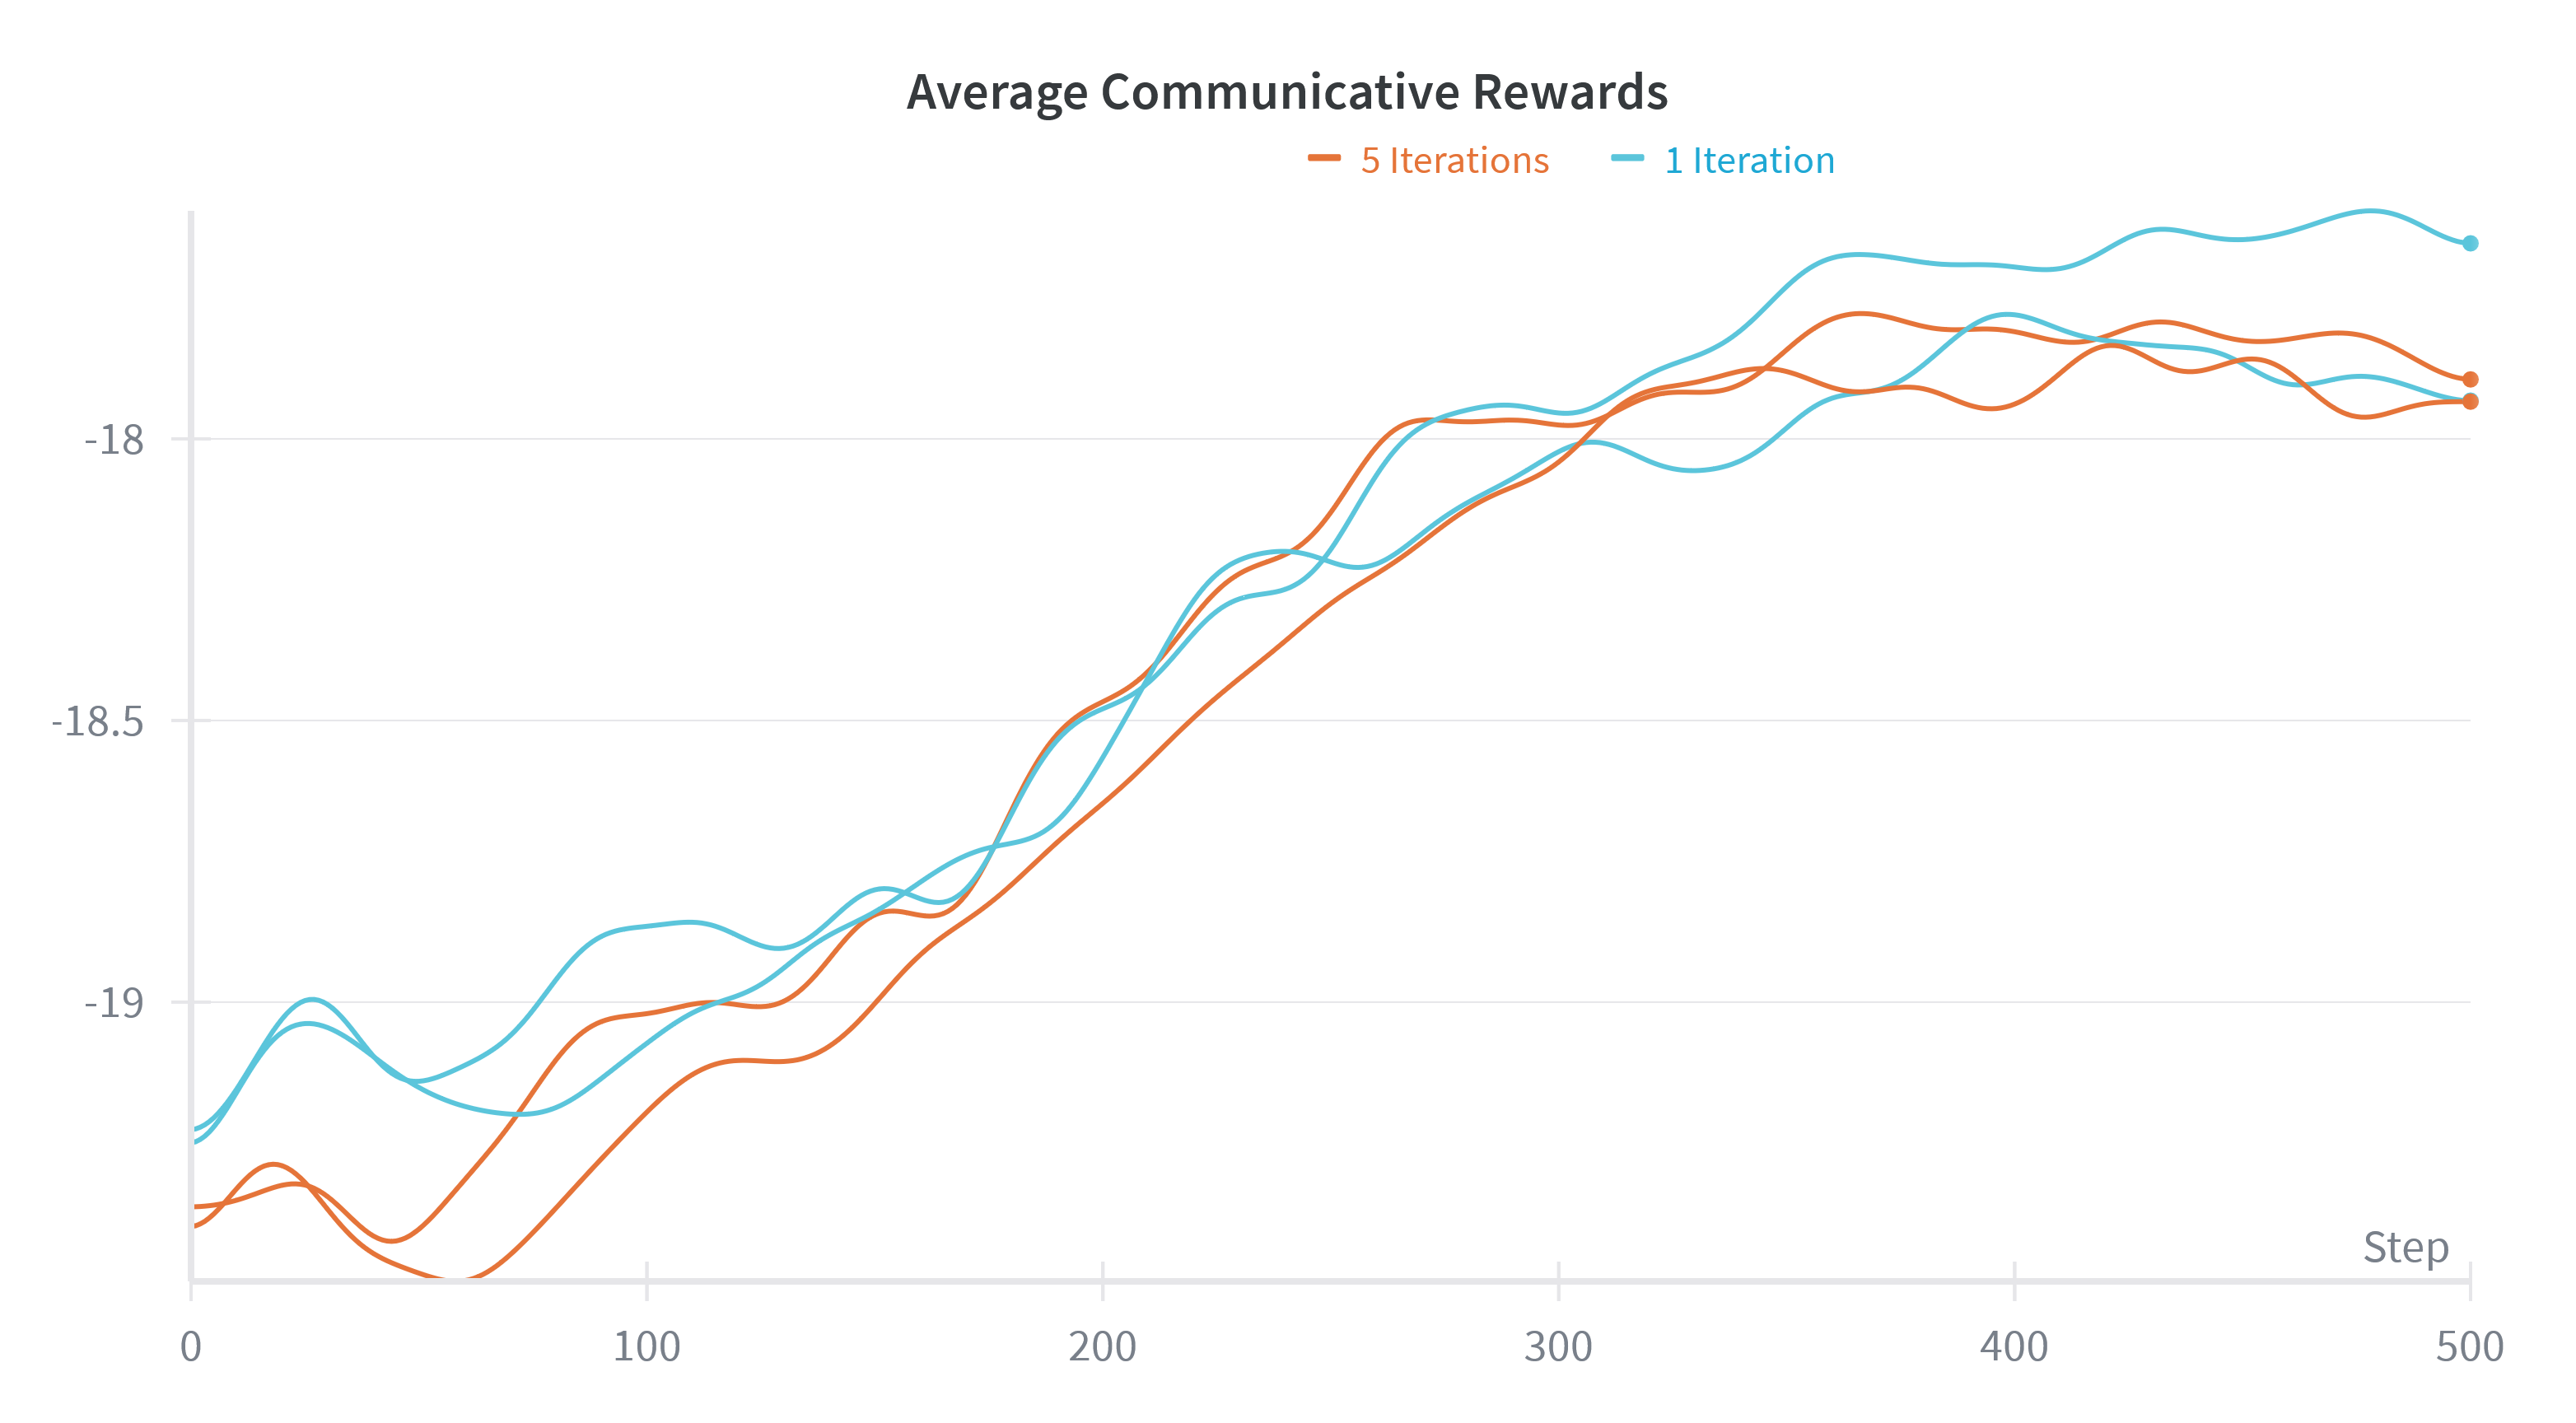
\includegraphics[width=0.8\textwidth]{img/n_iterations.png}
    \caption{Mean Communicative Reward ($\Rcomm$) for different iterative depths.}
    \label{fig:n_iterations}
\end{figure}

As shown in Figure \ref{fig:n_iterations}, the number of recursive pragmatic iterations ($N_r$) has almost no discernible effect on the agent's ability to optimize the communicative reward. While increasing iterations technically sharpens the listener's posterior distribution, this effect is functionally similar to increasing the listener's temperature $\alpha_{\text{temp}}$. Given that our default temperature ($\alpha=20$) is already quite high, this additional sharpening appears to be redundant and provides no additional learning signal.

\section{Value of $\lambda$}

\begin{figure}[h!]
    \centering
    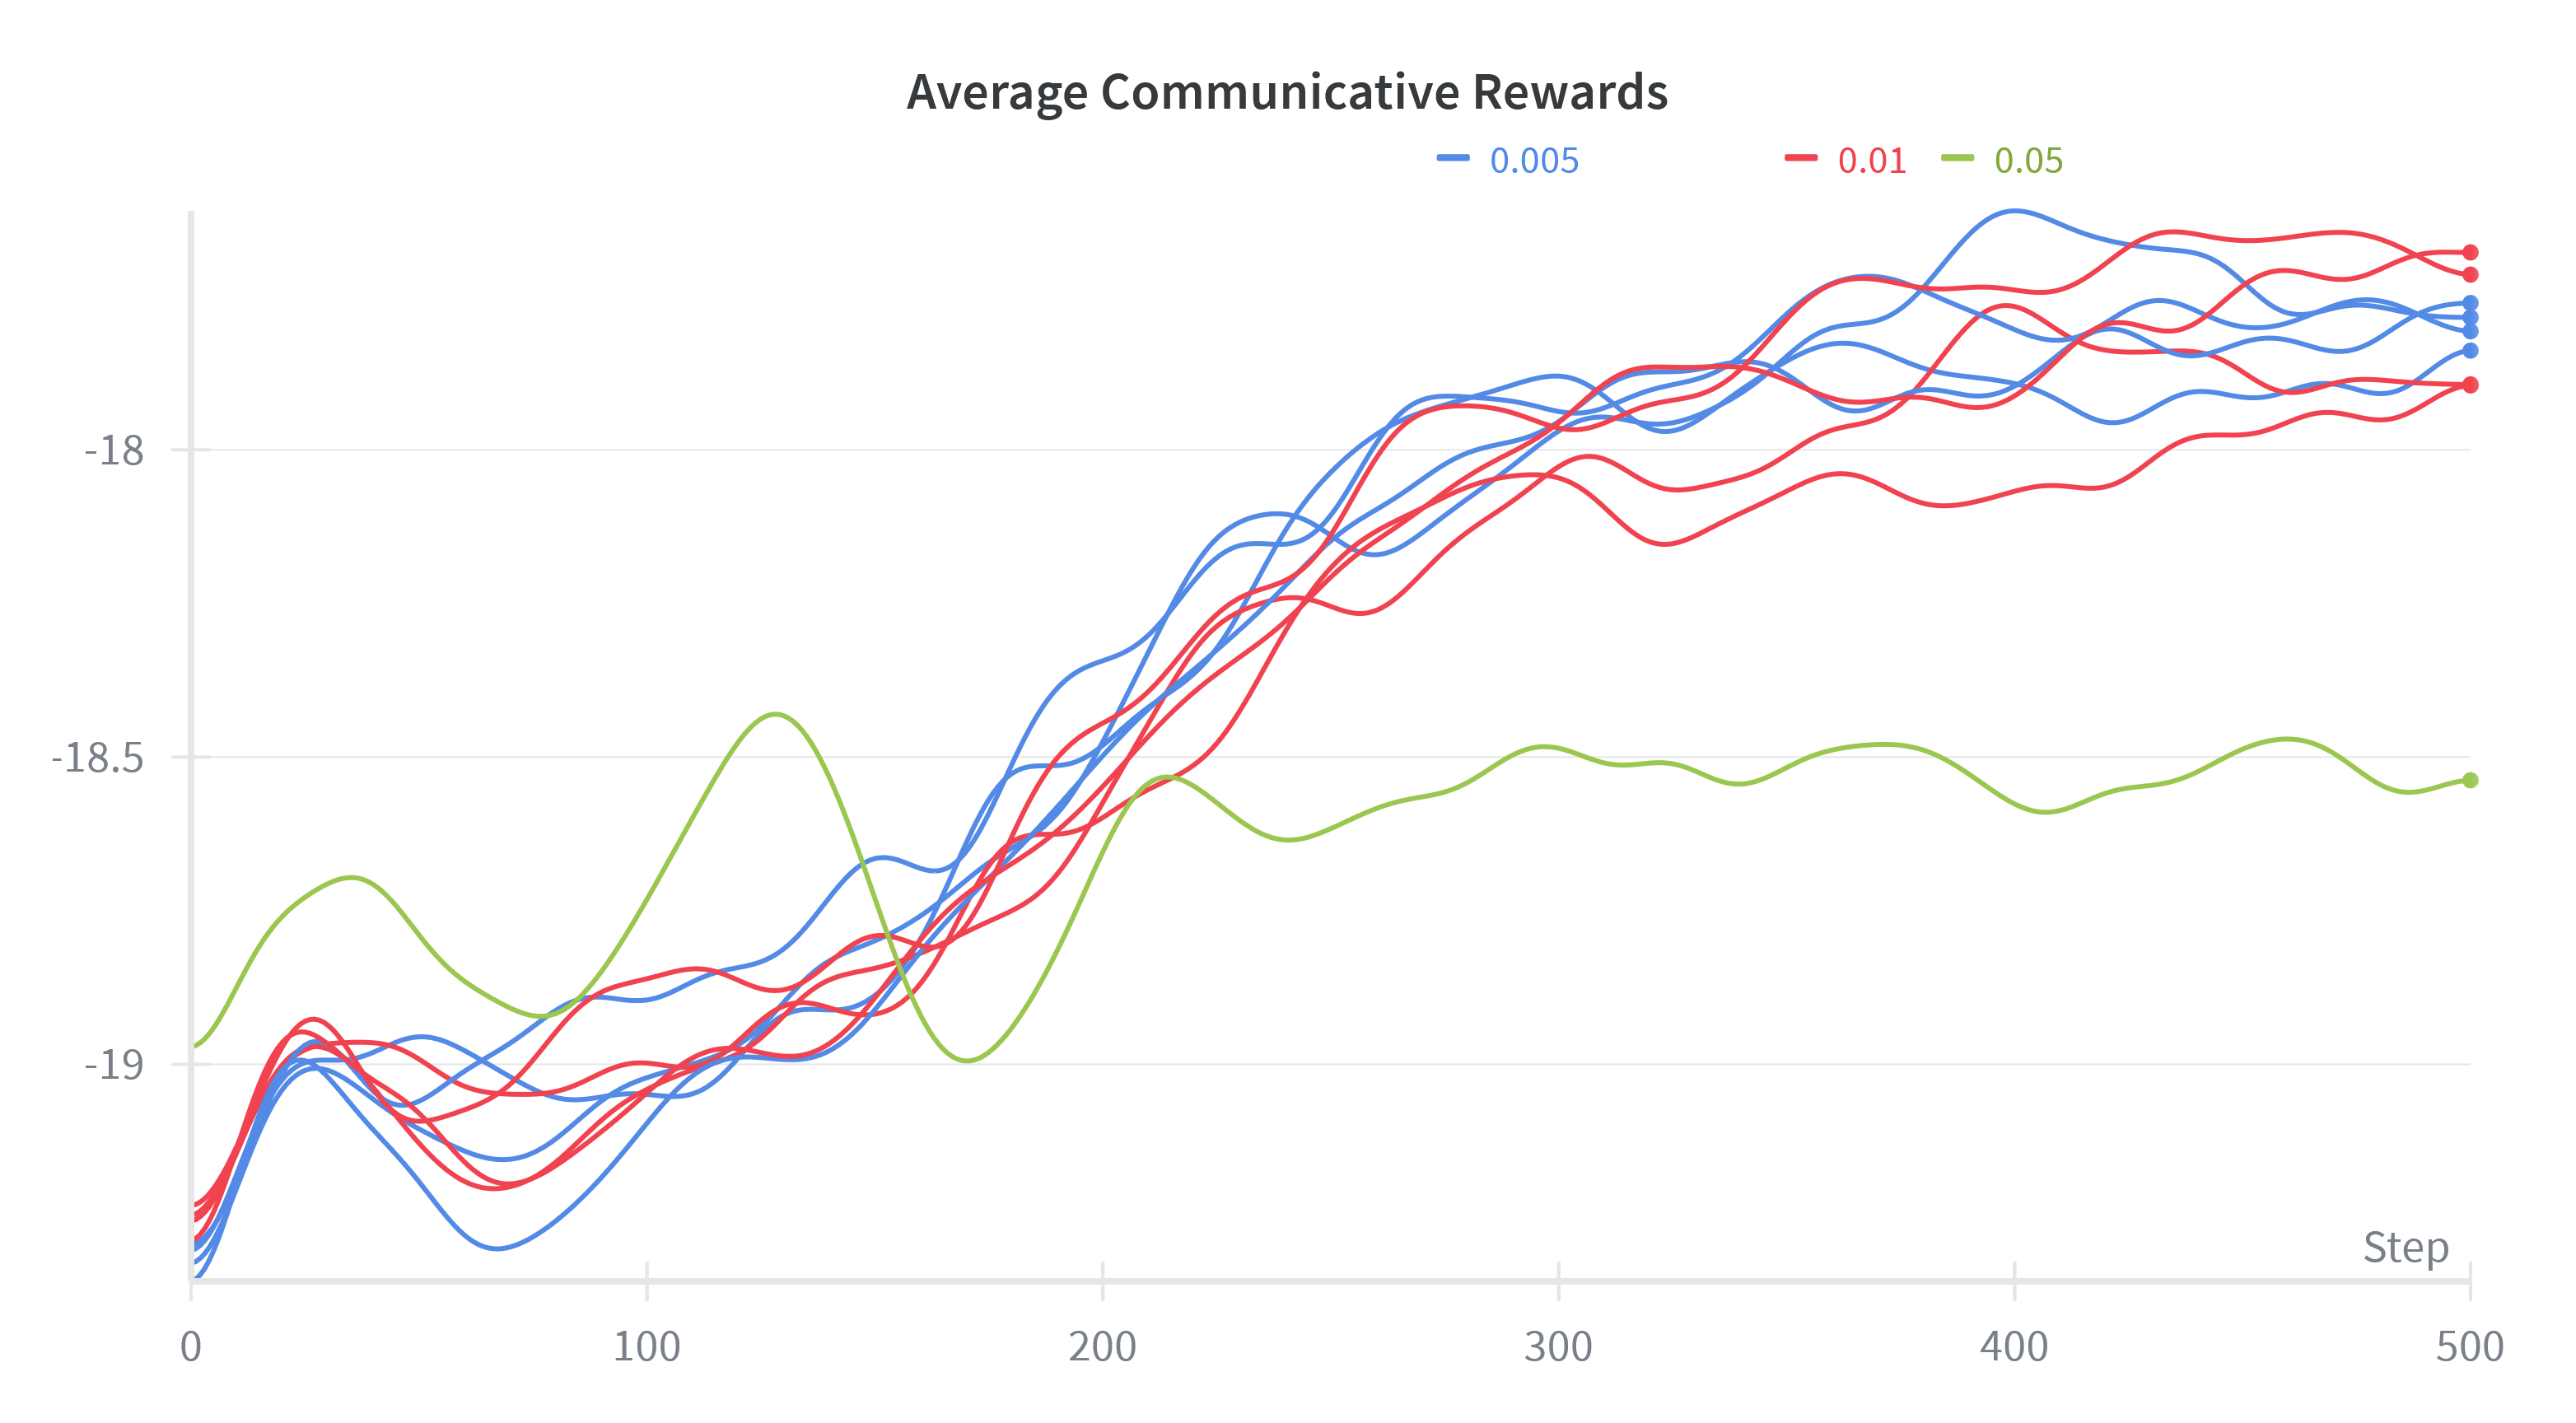
\includegraphics[width=0.8\textwidth]{img/lambda_crw.png}
    \caption{Mean Communicative Reward ($\Rcomm$) for different values of lambda.}
    \label{fig:lambda_crw}
\end{figure}

\begin{figure}[h!]
    \centering
    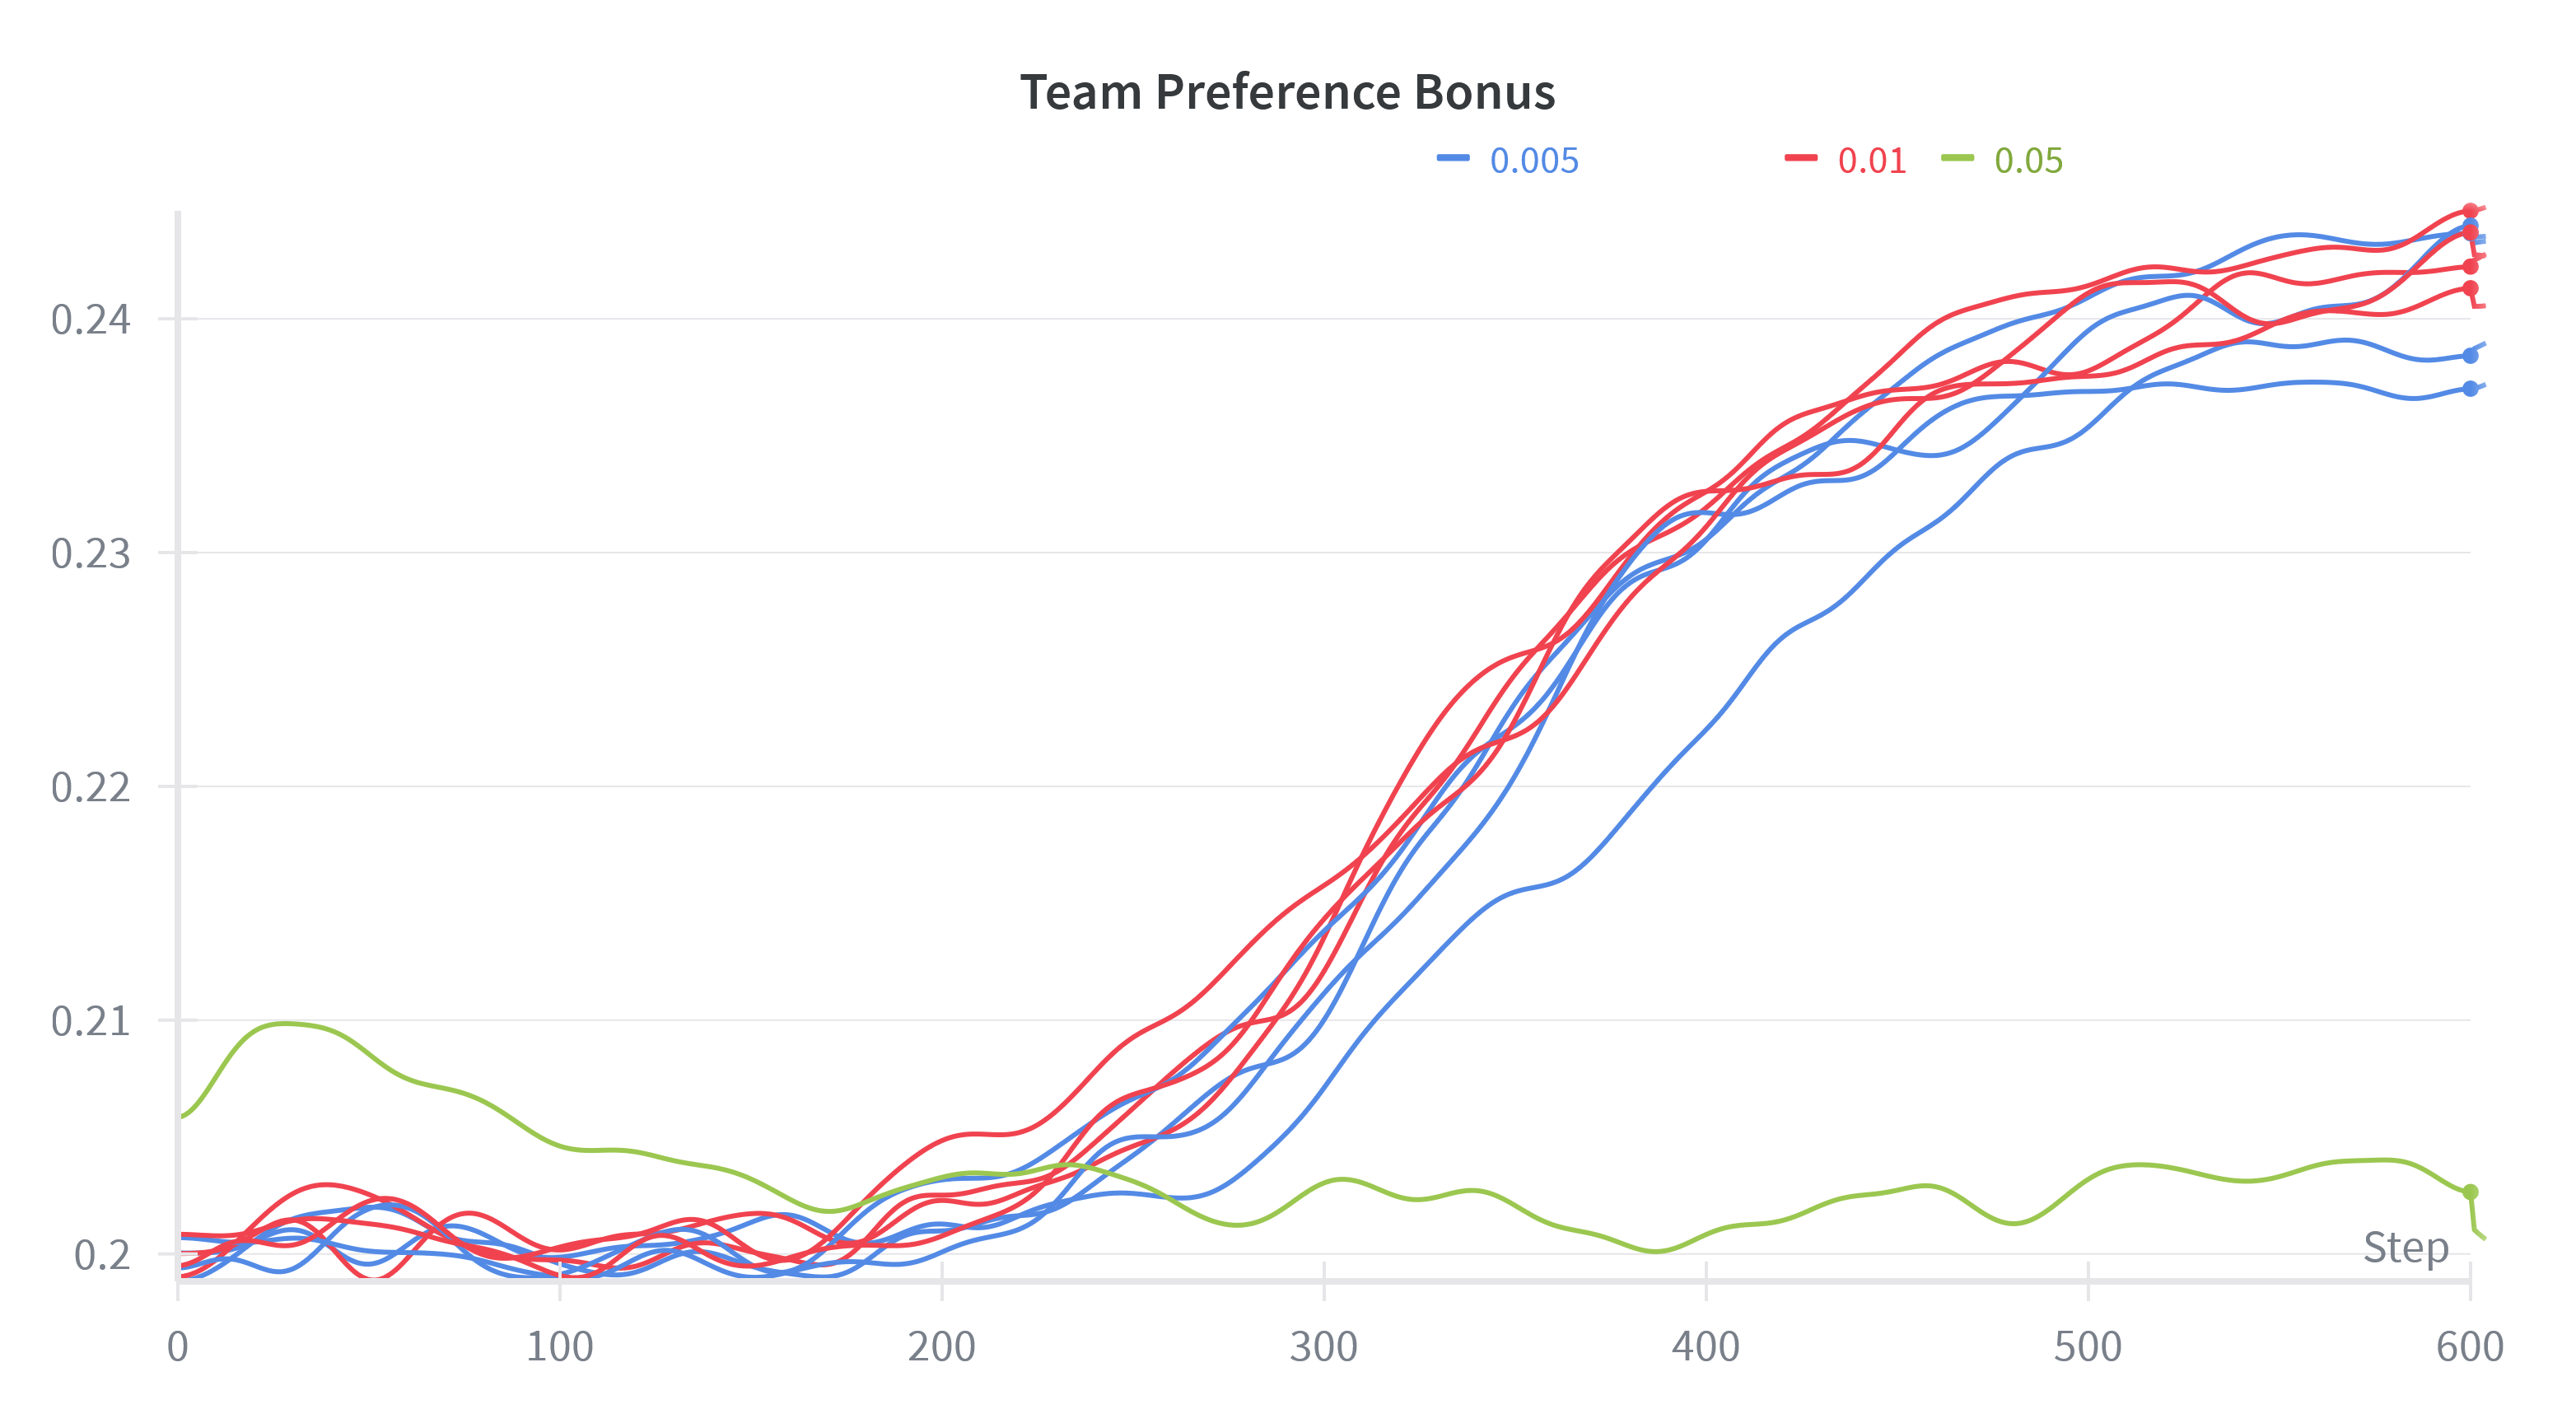
\includegraphics[width=0.8\textwidth]{img/lambda_tpf.png}
    \caption{Mean Team Preference Bonus for different values of lambda.}
    \label{fig:lambda_tpf}
\end{figure}

The weighting of the pragmatic reward, $\lambda$, is a highly sensitive hyperparameter. As shown in Figures \ref{fig:lambda_crw} and \ref{fig:lambda_tpf}, very small values of $\lambda$ (e.g., $0.005$) render the intrinsic reward irrelevant; it is treated as noise by the agent and is easily ignored in favor of the extrinsic task reward. Conversely, even a modest value like $0.05$ (our chosen value) appears to "nuke" the model's performance. The intrinsic reward signal dominates and conflicts with the extrinsic reward, preventing the agent from learning an effective task policy.

\end{document}